% ====================================================================

% LSST Observing Strategy White Paper

% Copyright 2015 The LSST Science Collaborations

% ====================================================================

\documentclass[11pt,headsepline,cleardoubleempty,twoside,openright]{scrbook}
% 11pt font
% Draw a line under the header
% Don't draw a line or print page numbers when a page is empty
% Pages are two-sided - so margins alternate
% Chapters start on the righthand side of the page
\pdfoutput=1
\usepackage{LSST_Observing_Strategy_White_Paper}


% ====================================================================

\begin{document}

\begin{titlepage}
\begin{center}

\vspace*{\stretch{2}}

{\Huge\bfseries\scshape
 Science-Driven Optimization \\ \vspace{\baselineskip}
 of the LSST Observing Strategy}

\vspace*{\stretch{2}}

\vspace*{\stretch{2.5}}

{\Large  Prepared by the LSST Science Collaborations,}\\
\vspace*{\stretch{0.15}}
{\Large with support from the LSST Project. }\\
\vspace*{\stretch{1}}

\input{thisversion.tex}

\end{center}
\end{titlepage}

% --------------------------------------------------------------------

\clearemptydoublepage
% Author list

\vspace{4\baselineskip}

\noindent{\href{https://github.com/LSSTScienceCollaborations/ObservingStrategy/graphs/contributors}{\LARGE\bf Contributing Authors}}

\vspace{\baselineskip}

% List of institutions:
\def\adler{Adler Planetarium, \ldots}
\def\aims{African Institute for Mathematical Sciences, 6 Melrose Road, Muizenberg 7945, South Africa}
\def\arizona{U of Arizona, \ldots}
\def\berkeley{Physics Division, Lawrence Berkeley National Laboratory, 1 Cyclotron Road, Berkeley, CA, 94720}
\def\caltech{California Institute of Technology, \ldots}
\def\centrallancashire{University of Central Lancashire, UK, \ldots}
\def\cfa{Harvard-Smithsonian Center for Astrophysics, \ldots}
\def\chicago{Department of Astronomy and Astrophysics, University of Chicago, 5640 South Ellis Avenue, Chicago, IL 60637, USA}
\def\cmu{Carnegie Mellon University, \ldots}
\def\columbia{Columbia, \ldots}
\def\cuny{CUNY, \ldots}
\def\ctio{Cerro Tololo Inter-American Observatory, La Serena, Chile}
\def\dearborn{University of Michigan-Dearborn, \ldots}
\def\delaware{University of Delaware, \ldots}
\def\drexel{Drexel University, \ldots}
\def\ennu{NU, \ldots}
\def\floridagulf{Florida Gulf Coast University, \ldots}
\def\goddard{NASA Goddard Space Flight Center, \ldots}
\def\harvard{Department of Physics \& Department of Astronomy, 17 Oxford Street, Harvard University, Cambridge MA 02138}
\def\ifa{Institute for Astronomy, Honolulu, HI \ldots}
\def\ipac{IPAC, \ldots}
\def\jpl{Jet Propulsion Laboratory, California Institute of Technology, 4800 Oak Grove Drive, Pasadena, CA 91109, USA, \ldots}
\def\kavli{Kavli Institute for Cosmological Physics, University of Chicago, Chicago, IL 60637, USA}
\def\lcogt{LCOGT, University of California, Santa Barbara, CA \ldots}
\def\lpc{Laboratoire de Physique de Clermont, IN2P3/CNRS, 63178 Aubière Cedex}
\def\lsst{LSST, \ldots}
\def\mssl{Mullard Space Science Laboratory (MSSL), University College London (UCL), Surrey RH5 6NT, UK}
\def\msu{Michigan State, \ldots}
\def\nso{National Solar Observatory, \ldots}
\def\noao{NOAO, \ldots}
\def\nyu{Center for Cosmology and Particle Physics, Department of Physics, New York University, 726 Broadway, 9th Floor, New York, NY 10003, USA}
\def\okc{The Oskar Klein Centre for Cosmoparticle Physics, Stockholm University, Stockholm, Sweden}
\def\osu{Ohio State University, \ldots}
\def\oswego{State University of New York at Oswego, \dots}
\def\oxford{University of Oxford, UK, \ldots}
\def\penn{University of Pennsylvania, \ldots}
\def\pitt{Physics and Astronomy Department, University of Pittsburgh, Pittsburgh, PA 15260, USA}
\def\princeton{Department of Astrophysical Sciences, Princeton University, Princeton, NJ 08544, USA}
\def\rutgers{Department of Physics and Astronomy, Rutgers the State University of New Jersey, 136 Frelinghuysen Road, Piscataway, NJ 08854 USA}
\def\uc{Department of Astronomy and Astrophysics, University of California, Santa Cruz, CA 95064, USA}
\def\scsu{Southern Connecticut State University, \ldots}
\def\seti{SETI Institute, 189 N. Bernardo Ave., Mountain View, CA 94043}
\def\ska{SKA South Africa, 3rd Floor, The Park, Park Road, Pinelands 7405, South Africa}
\def\sofia{SOFIA Science Center, NASA Ames Research Center, MS211-1, Moffett Field, CA 94035}
\def\slac{SLAC National Accelerator Laboratory, 2575 Sand Hill Road, MS29, Menlo Park, CA 94025, USA}
\def\somewhere{Some Institute, Somewhere, \ldots}
\def\stanford{Physics Department, Stanford University, Stanford, CA, 94305, USA}
\def\stsci{STScI, \ldots}
\def\texastech{Texas Tech University, \ldots}
\def\toronto{Dunlap Institute and Department of Astronomy and Astrophysics, University of Toronto, 50 St George Street, Toronto M5S 3H4, Canada}
\def\ucd{University of California, Davis, \ldots}
\def\ucl{Department of Physics and Astronomy, University College London, Gower Street, London WC1E 6BT, UK}
\def\unab{UNAB, Chile, \ldots}
\def\unt{University of North Texas, \ldots}
\def\usno{USNO, \ldots}
\def\utaustin{University of Texas at Austin, \ldots}
\def\uw{University of Washington, Department of Astronomy, University of Washington, Seattle, WA, 98195, USA}
\def\uwe{Department of Astronomy and the eScience Institute, University of Washington, Seattle, WA, 98195, USA}
\def\westernwash{Western Washington University, \ldots}
\def\vanderbilt{Vanderbilt University, \ldots}
\def\yale{Yale University, \ldots}



% List of authors:
\author{Phil Marshall}{drphilmarshall}{\slac}
\author{Scott Anderson}{ScottAnderson}{\somewhere}
\author{Timo Anguita}{tanguita}{\unab}
\author{Ruth Angus}{ruthangus}{\oxford}
\author{Iair Arcavi}{arcavi}{\lcogt}
\author{Humna Awan}{HumnaAwan}{\rutgers}
\author{Federica B.\ Bianco}{fedhere}{\nyu}
\author{Rahul Biswas}{rbiswas4}{\uwe}
\author{Keaton J. Bell}{keatonb}{\utaustin}
\author{Eric C.\ Bellm}{ebellm}{\caltech}
\author{David Bennett}{davidpbennett}{\goddard}
\author{Niel Brandt}{nielbrandt}{\somewhere}
\author{Chris Britt}{cbritt4}{\texastech}
\author{Derek Buzasi}{derekbuzasi}{\floridagulf}
\author{Dana I.\ Casetti-Dinescu}{DanaCD}{\scsu,~\yale}
\author{Laura Chomiuk}{chomiuk}{\msu}
\author{Will Clarkson}{willclarkson}{\dearborn}
\author{Chuck Claver}{cclaver}{\lsst}
\author{Andy Connolly}{connolly}{\uw}
\author{Kem Cook}{kem0cook}{\somewhere}
\author{James Davenport}{jimdavenport}{\westernwash}
\author{Victor Debattista}{vpdebattista}{\centrallancashire}
\author{Seth Digel}{sethdigel}{\slac}
\author{Zoheyr Doctor}{Doctor}{\ennu}
\author{Ryan Foley}{astrofoley}{\uc}
\author{Wen-fai Fong}{Fong}{\arizona}
\author{Llu\'is Galbany}{lgalbany}{\pitt}
\author{Eric Gawiser}{egawiser}{\rutgers}
\author{Mark Giampapa}{markgiampapa}{\nso}
\author{John E.\ Gizis}{jgizis}{\delaware}
\author{Melissa L.\ Graham}{MelissaGraham}{\uw}
\author{Carl Grillmair}{cgrillmair}{\somewhere}
\author{Phillipe Gris}{pgris}{\lpc}
\author{Zoltan Haiman}{Haiman}{\columbia}
\author{Patrick Hartigan}{phartigan}{\somewhere}
\author{Suzanne Hawley}{suzannehawley}{\uw}
\author{Ren\'{e}e Hlozek}{ReneeHlozek}{\toronto}
\author{\v{Z}eljko Ivezi\'{c}}{ivezic}{\uw}
\author{Saurabh W. Jha}{saurabhwjha}{\rutgers}
\author{C.\ Johns-Krull}{CJohnsKrull}{\somewhere}
\author{Lynne Jones}{rhiannonlynne}{\uw}
\author{Shashi Kanbur}{ShashiKanbur}{\oswego}
\author{Vassiliki Kalogera}{Kalogera}{\ennu}
\author{Vinay Kashyap}{vinaykashyap}{\cfa}
\author{Vishal Kasliwal}{AstroVPK}{\penn}
% \author{Someonecalled Knawro}{knawro}{Some Institute, Somewhere, \ldots}
\author{Richard Kessler}{RickKessler}{\kavli, \chicago}
\author{Alex Kim}{AlexGKim}{\berkeley}
\author{Peter Kurczynski}{pkurczynski}{\somewhere}
\author{Michael C.\ Liu}{mliu}{\ifa}
\author{Michelle Lochner}{MichelleLochner}{\aims, \ska, \ucl}
\author{Michael B.\ Lund}{lundmb}{\vanderbilt}
\author{Ashish Mahabal}{AshishMahabal}{\somewhere}
\author{Alex Malz}{aimalz}{\nyu}
\author{Raffaella Margutti}{raffaellamargutti}{\nyu}
\author{Tom Matheson}{tmatheson}{\noao}
\author{Jason McEwen}{jasonmcewen}{\mssl}
\author{Peregrine McGehee}{pmmcgehee}{\ipac}
\author{S{\o}ren Meibom}{sorenmeibom}{\cfa}
\author{Josh Meyers}{jmeyers314}{\stanford}
\author{Dave Monet}{dgmonet}{\usno}
\author{David Nidever}{dnidever}{\lsst}
\author{Knut Olsen}{knutago}{\noao}
\author{Eric Neilsen}{ehneilsen}{\somewhere}
\author{Jeffrey Newman}{janewman-pitt-edu}{\pitt}
\author{Hiranya Peiris}{hiranyapeiris}{\ucl, \okc}
\author{Matthew T.\ Penny}{mtpenny}{Sagan Fellow,~\osu}
\author{Christina Peters}{cmp346}{\drexel}
\author{Rados{\l}aw Poleski}{poleski}{\osu}
\author{Kara Ponder}{kponder}{\pitt}
\author{Gordon Richards}{GordonRichards}{\drexel}
\author{Stephen Ridgway}{StephenRidgway}{\noao}
\author{Jeonghee Rho}{jhrlsst}{\seti, \sofia}
\author{Jason Rhodes}{jasondrhodes}{\jpl}
\author{David Rubin}{rubind}{\stsci}
\author{Samuel Schmidt}{SamSchmidt}{\ucd}
\author{Robert Schuhmann}{rlschuhmann}{\ucl}
\author{Ohad Shemmer}{ohadshemmer}{\unt}
\author{Avi Shporer}{shporer}{\jpl}
\author{Colin Slater}{ctslater}{\uw}
\author{Nathan Smith}{nathansmith}{\arizona}
\author{Marcelles Soares-Santos}{soares-santos}{\somewhere}
\author{Keivan Stassun}{stassun}{\vanderbilt}
\author{Jay Strader}{caprastro}{\msu}
\author{Michael Strauss}{michaelstrauss}{\princeton}
\author{Rachel Street}{}{\lcogt}
\author{Christopher Stubbs}{astrostubbs}{\harvard}
\author{Paula Szkody}{paulaszkody}{\uw}
\author{David Trilling}{davidtrilling}{\somewhere}
\author{Virginia Trimble}{Trimble}{\somewhere}
\author{Tony Tyson}{tonytyson}{\ucd}
\author{Miguel de Val-Borro}{migueldvb}{\princeton}
\author{Stefano Valenti}{svalenti}{\somewhere}
\author{Kathy Vivas}{akvivas}{\ctio}
\author{Robert Wagoner}{wagoner@stanford.edu}{\stanford}
\author{Lucianne Walkowicz}{lmwalkowicz}{\adler}
\author{Beth Willman}{bethwillman}{\lsst}
\author{Michael W. Wood-Vasey}{wmwv}{\pitt}
\author{Peter Yoachim}{yoachim}{\somewhere}
\author{Bevin Ashley Zauderer}{Zauderer}{\nyu}
\author{Matt O'Dowd}{mattodowd}{\cuny}
% {\it your name here},
% {and the LSST Project and Science Collaborations}


% --------------------------------------------------------------------

\tableofcontents
\label{toc}

% --------------------------------------------------------------------

\clearemptydoublepage
\setcounter{chapter}{0}
\chapter*{Preface}
\def\chpname{preface}\label{chp:\chpname}
\addcontentsline{toc}{section}{Preface}
\markboth{}{}

\noindent This is a community white paper outlining various science
cases and the impacts that observing strategy will have on them,
quantified using the Metric Analysis Framework. We will describe
various strategies and tradeoffs that impact the observing cadence
(visit sequence), the current cadence baseline, and future directions
for the optimization of the survey strategy. We aim to publish this
white paper on arXiv, and invite community feedback.

The timescale for producing this white paper, started before and
finished after the Observing Strategy workshop at the  August 2015
LSST Project and Community workshop, is many months.

% --------------------------------------------------------------------

\section*{Messages}
% \addcontentsline{toc}{subsection}{Messages}

The main points we aim to convey in this white paper are as follows:

\begin{itemize}

    \item We have a pretty good idea of how we would deploy LSST:
    there is a baseline strategy and a corresponding  simulated visit
    sequence, with which it can be demonstrated that the data required
    for the promised science can be delivered.

    \item However, the baseline strategy is not set in stone, and
    can and will be optimized. Even small changes could
    result in significant improvements to the overall science yield.

    \item These improvements can be predicted via analysis of the
    outputs of the LSST Operations Simulator, \OpSim, using the
    Metric Analysis Framework (\MAF). Once the baseline visit sequence
    has been evaluated with a given science case's metrics, all other
    proposed visit sequences can be compared against it, automatically.

    \item The LSST observing strategy evaluation and optimization
    process will be as open and inclusive as possible. We invite all
    stakeholders to participate.

\end{itemize}

%\raggedright{Project start: July 2015.}
Project start: July 2015.

\clearpage

% --------------------------------------------------------------------

\section*{Guidelines for Authors}
\addcontentsline{toc}{section}{Guidelines for Authors}
\def\secname{guidelines}\label{sec:\secname}

\noindent{\it Phil Marshall}
%(\texttt{@drphilmarshall})

Since this is a community white paper, contributions are welcome from
everyone. Read on for how to make a contribution, and how you should
structure that contribution.

\subsection{How to Get Involved}

The first thing you should do is read and absorb the current version
of the white paper, which you should be able to
\href{http://ls.st/iw2}{view on \GitHub}. (You can also
\href{https://github.com/LSSTScienceCollaborations/ObservingStrategy/raw/master/whitepaper/LSST_Observing_Strategy_White_Paper.pdf}{download
the ``raw'' PDF}, which is hyper-linked for easier navigation.) You
will then be able to provide good feedback, which you should do via
the
\href{https://github.com/LSSTScienceCollaborations/ObservingStrategy/issues}{\GitHub
issues}. Browse the existing issues first: there might be a
conversation you can  join. New issues are most welcome: we'd like to
make this white paper as comprehensive as possible.

To edit the white paper, you'll need to
\href{https://help.github.com/articles/fork-a-repo/}{``fork'' its
repository}. You will then  be able to edit the paper in your own
fork, and when you are ready,  submit a
\href{https://help.github.com/articles/using-pull-requests/}{``pull
request''} explaining what you are doing and the new version that  you
would like to be accepted. It's a good idea to submit this pull
request sooner rather than later, because associated with it will be a
discussion thread that the writing community can use to discuss your
ideas with you. For help getting started with \git and \GitHub, please
see this
\href{https://github.com/drphilmarshall/GettingStarted#top}{handy
guide}.


\subsection{Chapter and Section Design}

For a high-level justification of the following design, please see
\autoref{sec:intro:evaluation}. In short, we're aiming for modular
sections (that are easy to write in parallel, and then re-arrange
within chapters later) focused on one science project each, and
quantified by one (or maybe two) figures of merit (which will likely
depend on other, lower-level metrics). Each section can be thought of
as an observing proposal, demonstrating the performance achievable
given various assumptions about the time awarded.\footnote{These notes
on the white paper design are adapted from the notes at
\href{https://github.com/LSSTScienceCollaborations/ObservingStrategy/blob/master/whitepaper/notes/chapter-template.md}{\texttt{whitepaper/notes/chapter-template.md}}}


The first section of each science chapter needs to be an \textit{introduction}
that outlines, very briefly, the commonality of the key science projects
contained in it:  what is to be measured, in broad-brush terms, and
why this is of interest. Then, suppose we were to design an LSST
survey to enable these measurements: qualitatively, what might it look
like, in terms of the choices we are able to make? This chapter
introduction can eventually (when the results are in!) summarize,
again, in very broad brush terms, the results of a number of
investigative sections, one on each science case.

The individual sections following this introduction will then need to
describe the particular discoveries and measurements that are being
targeted in each \textit{science case}. It will be helpful to think of a
``science case" as a ``science project" that the section leads {\it
actually plan to do}. Thinking this way means that the sections can
follow the tried and tested format of an observing proposal: a brief
description of the investigation, with references, followed by a
technical feasibility piece.


\subsection{Metric Quantification}

\new{\bf The assessment of each science case will need to be
quantified using the MAF framework, via a set of metrics that need to
be computed for any given observing strategy in order to quantify its
impact on the described science.}

\new{Ideally, these metrics would be combined in a \textit{well-motivated
figure of merit}, and used to compare several possible observing
strategies (that have already been simulated with \OpSim). In many (or
perhaps all) cases,  a figure of merit will be a \textit{precision} (\ie
a percentage statistical uncertainty) on a astrophysical model
parameter, assuming negligible bias in its inference. Precision is
usually what we need to forecast in order to convince TAC's to give us
telescope time, and so it makes sense to focus on it here too.}

\new{Early on in a metric analysis, it may not be possible to compute
a science case's ideal figure of merit, most likely because to do do
would require a large simulation program to capture the response of
the  parameter measurement to the observing strategy. At this early
stage, it makes sense to look for simple proxies that \textit{scale} the
same way as model parameter precision. For example, we might expect
the precision on a set of luminosity function  parameters to scale
with the square root of the number of objects in the sample, and so
$\sqrt{N}$ could be a sensible early figure of merit. Provided we get
the scaling right, \textit{we can then compare different observing
strategies by looking  at the percentage change in the figure of
merit,} and arguing that  this will correspond approximately to the
same percentage change in the  ideal case.}

Each science section needs to conclude with a discussion of any risks
that have been identified, and how these could be mitigated. \new{What does
this mean? Each science project will have a \textit{threshold acceptable
figure of merit value}, as well as a target (or ``design'') value.  If
an observing strategy gives a figure of merit below the threshold, it
is very important that we know about it.  Optimizing all science cases
in such a complex and diverse set is not really the best way of
thinking about LSST's scheduling task: \textit{rather than maximizing
happiness, what we are really trying to do is minimze global
unhappiness (Z.~Ivezic, priv.\ comm.).}}

\textit{The comparisons between different simulated
strategies will help make the case for any changes to the baseline
strategy, and in the short term provide motivation for
\href{https://github.com/LSSTScienceCollaborations/ObservingStrategy/blob/master/opsim/README.md}{proposed
new \OpSim simulation runs.}} \new{For some science sections we will
have only a metric design, without an implementation. Subsequent
versions of this white paper will hopefully see these designs realized
and put into action. For now, though, the discussion of risks to these
science cases will necessarily be minimal, containing only predictions
for how the figure of merit will vary among observing strategies.}

\new{Quantitative comparisons between science cases needs will be
carried out in the final chapter, ``Tensions and Trade-offs.'' This
chapter cannot be written until we have quantitative MAF metric
analysis results from the individual science cases to feed into it. At
this early stage, the metrics for each science case, and in
particular, the figures of merit, are not yet well defined. Again,
rather than wait for the ideal figure of merit, \textit{we instead
encourage the calculation of simple proxies} that can give at least
some early information about how good the baseline strategy and its
early perturbations will be for each science case.}

The following chapter shows a template introduction and
science case section for you to work from. The latter is checked into
the repository as
\href{https://github.com/LSSTScienceCollaborations/ObservingStrategy/blob/master/whitepaper/section-template.tex}{\texttt{section-template.tex}}.
For an example of a section being developed according to the above guidelines,
please take a look at \autoref{sec:lenstimedelays}.


% ====================================================================

\setcounter{chapter}{-1}
\chapter{Template Science Chapter}
\def\chpname{example}\label{chp:\chpname}

\noindent {\it
Editor Name(s)
}

% --------------------------------------------------------------------

\section{Introduction}
\label{sec:\chpname:intro}

General introduction to the chapter's science projects.

Overview of observing strategy needed by those projects, bringing
out common themes or points of tension.

% --------------------------------------------------------------------

\input{section-template}

% --------------------------------------------------------------------


% --------------------------------------------------------------------

\clearemptydoublepage
\setcounter{chapter}{0}
\chapter*{Summary}
\def\chpname{summary}\label{chp:\chpname}
\addcontentsline{toc}{section}{Summary}
\markboth{}{}

% Short (c. 250 word) summary for arxiv posting:

\noindent
The Large Synoptic Survey Telescope is designed to provide a single
cataloged optical imaging database that will support investigation of
our Solar System, Galaxy and Universe, across half the sky and over ten
years of repeated observation.
%
However, exactly how the LSST observations are taken (the observing strategy or ``cadence'') is not yet finalized.
%
In this dynamically-evolving community white paper, we explore how the
detailed performance of the anticipated science investigations is
expected to depend on small changes to the LSST observing strategy.
%
Using realistic simulations of the LSST schedule and observation
properties, we design and compute diagnostic metrics and Figures of
Merit that provide quantitative evaluations of different observing
strategies, analyzing their impact on a wide range of proposed science
projects.
%
This is work in progress: we are using this white paper to communicate
to each other the relative merits of the observing strategy choices that
could be made, in an effort to maximize the scientific value of the
survey.
%
The investigation of some science cases leads to suggestions for new
strategies that could be simulated and potentially adopted.
%
Notably, we find motivation for exploring departures from a spatially
uniform annual tiling of the sky: focusing instead on different parts of
the survey area in different years in a ``rolling cadence'' is likely to
have significant benefits for a number of time domain and moving object
astronomy projects.
%
The communal assembly of a suite of quantified and homogeneously coded
metrics is the vital first step towards an automated, systematic,
science-based assessment of any given cadence simulation, that will
enable the scheduling of the LSST to be as well-informed as possible.

\clearpage


% --------------------------------------------------------------------

% The v2 introduction should explain the structure of the paper,
% and describe the 2018 white paper process.

\chapter[Introduction]{Introduction}
\def\chpname{intro}\label{chp:\chpname}

Chapter editors:
\credit{bethwillman},
\credit{connolly}.

The Large Synoptic Survey Telescope (LSST) is a dedicated optical
telescope with an effective aperture of 6.7 meters, currently under
construction on Cerro Pach\'on in the Chilean Andes.  The telescope
and camera will have a huge field of view, 9.6 deg$^2$, and the
\'etendue, i.e., the product of collecting area and field of view will
be significantly larger than any other optical telescope.  Thus this telescope
is designed for wide-field deep imaging of the sky; its mantra is
``Wide-Deep-Fast'', i.e., the ability to cover large swaths of sky
(``Wide'') to faint magnitudes (``Deep'') in a short amount of time
(``Fast''), allowing it to scan the sky repeatedly.  LSST will image
in six broad filters, $ugrizy$, spanning the optical band from the
atmospheric cutoff in the ultraviolet to the limit of CCD sensitivity
in the near-infrared.  

  The science case for the LSST is based broadly on four science
  themes:
\begin{itemize}
\item Dark energy and dark matter (via measurements of strong and weak lensing,
  large-scale structure, clusters of galaxies, and supernovae);
\item Exploring the transient and variable universe;
\item Studying the structure of the Milky Way galaxy and its neighbors
  via resolved stellar populations;
\item An inventory of the Solar System, including Near Earth Asteroids
  and Potential Hazardous Objects, Main Belt Asteroids, and
  Kuiper Belt Objects.
\end{itemize}

These themes, together with {\em many} other science applications, are
described in detail in the
\href{http://lsst.org/scientists/scibook}{LSST Science Book}, produced
by the LSST Project Team and Science collaborations in 2009.  The
present white paper represents an important next step in science
planning beyond the Science Book.  In particular, we now need to
quantify how well the LSST (for a given realization of its observing
strategy, or ``{\em cadence}'') will be able to carry out its science
goals; indeed, we will use this quantification to refine and optimize
the cadence itself.  To zeroth order, the large \'etendue of LSST
allows it to meet all its science goals with a single dataset with a
universal cadence.  This document describes the design of the LSST
cadence and the various ways in which can be further refined to
optimize the science output of the survey.  As we describe in detail
below, we quantify the effectiveness of a given cadence realization to
meet science goals by defining a series of quantitative {\em metrics}.
Any given realization will be more favorable for some science areas,
and less so for others; the metrics allow us to quantify this, and
optimize the overall cadence for the broadest range of LSST science
areas.

In the six years since the Science Book was written, some of the
science themes described in there have evolved or become obselete,
while new science opportunities and ideas have arisen.  Moreover, our
understanding of the capabilities (such as system response and
therefore depth, telescope optics, and so on) have matured
considerably.  The present document endeavors to explore the principal
science themes as described in the Science Book, but is not slaved to
them, and where appropriate, we will point out relevant updates to the
Science Book.



% --------------------------------------------------------------------

\section{Synoptic Sky Surveying at Universal Cadence}
\def\secname{intro:baseline}\label{sec:\secname}

  The LSST defined a so-called ``baseline cadence'', described in the
  \href{http://adsabs.harvard.edu/abs/2008arXiv0805.2366I}{LSST
    overview paper} and Chapter 3 of the Science Book.  This was used
  to demonstrate that LSST could meet its basic science goals, and
  indeed the formal
  \href{https://www.lsstcorp.org/docushare/dsweb/Get/LPM-17}{science
    requirements}.    As 
  described in these references, the default LSST exposure is 15
  seconds, and all exposures are taken in pairs, called a ``{\em
    visit}'', before the telescope is slewed to a neighboring field.
   Any given field is observed twice on a given night, which allows
   preliminary trajectories of asteroids to be determined.  

   The baseline cadence optimizes the amount of sky covered in any
   given night (subject to the constraint of observing at airmass less
   than 1.4 throughout), and allows the entire sky visible at any time
   of the year to be covered in about three nights.  The cadence is
   designed to give uniform coverage at any given time, and reaches
   survey goals for measuring stellar parallax and proper motion over
   the ten-year survey.  The survey requirements on depth lead to
   roughly 825 visits (summing over the six filters) in the 10-year
   LSST survey to any given point on the sky.  The resulting
   Deep-Wide-Fast component of the survey covers roughly 18,000
   deg$^2$ of high Galactic latitude sky, and requires about 85\% of
   the available observing time. 

   There are obvious science cases that the Deep-Wide-Fast survey does
   not address, and thus the remaining 15\% of the telescope time in
   the baseline cadence is devoted to a series of specialized
   surveys.  They are as follows: 
\begin{itemize} 
\item Imaging at low Galactic latitudes.  This is currently defined as
  a wedge which is broader closer to the Galactic Center,
  corresponding roughly to a locus of constant stellar density.  In
  this region, the number of repeat observations is reduced, given the
  confusion limit in the stacked LSST data. 
\item Imaging in the South Celestial Cap.  The airmass limit of 1.4
  restricts observations to declination $> -70^\circ$ ({\bf get
    precise value}), thus missing both the Magellanic Clouds.
  Observations are done in the Cap to cover this region of sky, again
  to shallower depth. 
\item Imaging in a series of four {\em Deep Drilling Fields}, single
  pointings in which 
  we will obtain roughly four {\bf check!} times more exposures in all
  filters in order to go about a magnitude fainter in the stacked
  data, as well as to get better sampled light curves of variable
  objects. 
\item Imaging in the Northern portions of the Ecliptic Plane.  The
  airmass limit of 1.4 restricts us to declination $< +2^\circ$ ({\bf
    get precise value}), which means that much of the ecliptic plane
  is uncovered.  By observing with a reduced cadence close to the
  Ecliptic Plane north of this limit, we will be able to significantly
  increase the fraction of Near-Earth Asteroids and Main Belt
  Asteroids for which LSST obtains orbits.
\end{itemize}

  The LSST Project has developed an ``Operations Simulator'' (\OpSim),
  described in detail in Chapter~\ref{chp:cadexp} of this paper, which includes a
  realistic model of telescope operations, including time required for
  camera readout, slew time, filter exchange, as well as time loss due
  to clouds.  Given a series of ``proposals'' {\bf Do we still want to
    use this vocabulary?} that set priorities of which fields to
  observe at any given time, \OpSim has developed a series of
  realizations of the series of observations that make up the ten-year
  LSST survey.  Given such a realization, \OpSim outputs detailed
  metrics describing, for example, the expected depth of the LSST
  survey in each filter as a function of time.  The baseline cadence
  is a specific realization of the \OpSim output, which meets the LSST
  survey requirements, following the rules briefly outlined above.  
   
  Again, while the baseline cadence demonstrates that the LSST is
  capable of meeting its stated science goals, it is not optimized for
  all science, and Chapter~\ref{chp:cadexp} of this document describes a series of
  experiments varying the assumptions in \OpSim.  In
  Chapter~\ref{chp:specialsurveys}, we explore additional ideas for
  future experiments to be done in \OpSim.  

%Synoptic Surveying with LSST - the basic observing strategy determined
%by key projects described in the LSST Science Requirements Document,
%and constrained by the LSST's design \citep{IvezicEtal2008}.

% --------------------------------------------------------------------
\iffalse
THIS SECTION HAS BEEN ABSORBED INTO WHAT IS ABOVE.
\section{Beyond the Baseline Observing Strategy}
\def\secname{intro:baseline}\label{sec:\secname}

Optimizing the Observing Strategy: what perturbations are we
permitted to introduce, to maximize the system's science capabilities?
What are our constraints? And our opportunities?
\fi

% --------------------------------------------------------------------

\section{Evaluation and Optimization of the LSST Observing Strategy}
\def\secname{intro:evaluation}\label{sec:\secname}

The next step is to quantify how well any given realization of the
LSST observing strategy (i.e., an output of \OpSim) supports the (many)
science projects that LSST will enable.  As the algorithms controlling
\OpSim are varied, some projects will benefit, while others may
suffer.  By quantifying this for each projects, we can determine which cadence
maximizes the science potential overall of the project. 

Thus we need 
%e first step towards a science-based optimization of the LSST
%observing strategy is 
a {\it science-based evaluation of the baseline
  LSST observing strategy and its variants}. After simulating a sample
observing schedule consistent with this strategy (see
\autoref{chp:cadexp}), we then need to quantify its value to each
science team.  This is what the LSST DM Sims team's ``Metric Analysis
Framework'' was designed to enable. Once the fiducial strategy has
been evaluated in this way, then any other strategy can be evaluated
in the same terms, using the same code, and we will be able to %start
optimize the strategy through iterations between \OpSim and MAF.

With this program in mind, it makes sense to define {\it one ``Figure
of Merit'' (FoM) per science project}, that captures the value of  the
observing strategy under consideration to that science team. This FoM
will probably be a function of several ``metrics'' that quantify
lower-level features of the observing sequence.  For Figures of Merit
to be directly comparable between disparate science projects,  they
need to be dimensional, and have the same units. One natural
choice could be the {\it information gained} by the science team, in
bits. This is a well-defined statistical quantity, albeit not yet one
in common use. A given observing schedule's value would then depend on
both this information gain, but also {\it how much that information is
worth to the whole community}. It is at this point that the debate
could become heated: probably the best we can do in Cadence Diplomacy
is to quantify all the information gains implied by each proposed
change to the baseline  observing strategy, combine them to see
whether it makes everyone happy, and iterate. In this way we might
hope to minimize the debates about the less quantifiable worth of each
piece of information.

We are some way from being able to define information-based Figures of
Merit for most science cases -- but the metrics that they will depend
on will be easier to derive. Writing this white paper is an
opportunity to think through the Figure of Merit for each science
project that we as a community want to carry out, and how that measure
of success is likely (or even known) to depend on metrics that
summarize the observing sequence presented to us. Thinking about the
problem in terms of science projects, each with a  Figure of Merit,
encourages us to design modular document sections, with one science
project and one Figure of Merit per section.

{\bf I am not sure the following paragraph belongs in the white paper;
  it is more a description of the writing process.}

This will have the happy side-effect of allowing the chapters to be
straightforwardly re-arranged as we go, to make the white paper easier
to read. It will also naturally lead to the definition of a suite of
MAF  super-metrics, can be evaluated on any future \OpSim output
database.  A table in each section showing the values of the metrics
and the FoM, for different schedules, for that science project, will
be very helpful. The metric names in these tables should match the
metric class names in the
\href{https://github.com/LSST-nonproject/sims_maf_contrib/wiki}{\simsMafContrib}
module. In principle these tables could be auto-generated by the MAF
framework, and extended as \OpSim is repeatedly reconfigured and run.

For an example of how all this could look, please see the
\hyperref[sec:lenstimedelays]{lens
time delays section}. The MAF subsections are still under development
there, but keep checking back to see it come together during the
August 2015 workshop week. Templates for the chapters and sections can
be found in \autoref{chp:example}.


% --------------------------------------------------------------------

\section{Outline of This Paper}
\def\secname{intro:outline}\label{sec:\secname}

The rest of this white paper is structured as follows. In
\autoref{chp:cadexp} we describe a number of \OpSim simulated observing
schedules (``cadences'') explored by the LSST Sims team in summer 2015
in preparation for this paper: they include a ``baseline cadence'', and
then some small but interesting perturbations to it. Then, we present
the science cases considered so far, organised into the following
chapters:

\begin{itemize}
    \item \autoref{chp:solarsystem}: \nameref{chp:solarsystem}
    \item \autoref{chp:galaxy}: \nameref{chp:galaxy}
    % \item \autoref{chp:astrometry}: \nameref{chp:astrometry}
    \item \autoref{chp:variables}: \nameref{chp:variables}
    \item \autoref{chp:transients}: \nameref{chp:transients}
    \item \autoref{chp:MCs}: \nameref{chp:MCs}
    \item \autoref{chp:agn}: \nameref{chp:agn}
    \item \autoref{chp:cosmo}: \nameref{chp:cosmo}
    % \item \autoref{chp:deepdrilling}: \nameref{chp:deepdrilling}
    \item \autoref{chp:specialsurveys}: \nameref{chp:specialsurveys}
    \item \autoref{chp:wfirst}: \nameref{chp:wfirst}
\end{itemize}

Finally, in \autoref{chp:tradeoffs} we bring the results of all the
science metric analyses  together and discuss the tensions between
them, and the trade-offs that we can anticipate having to make.

\navigationbar

% --------------------------------------------------------------------


% --------------------------------------------------------------------

\part{Simulations}
\def\partname{sims}\label{part:\partname}

% v2 could have two chapters, for the two suite of simulations we
% now have:

% --------------------------------------------------------------------

\chapter[Some Example Observing Strategies]{The Operations Simulator and its Outputs}
\def\chpname{cadexp}\label{chp:\chpname}

Chapter editors:
\credit{ivezic},
\credit{yoachim},
\credit{rhiannonlynne}.

Contributing authors:
\credit{kem0cook},
\credit{StephenRidgway},
\credit{drphilmarshall}

% --------------------------------------------------------------------

\section*{Summary}
\addcontentsline{toc}{section}{~~~~~~~~~Summary}

In this chapter
%(which was originally prepared as \href{http://www.astro.washington.edu/users/ivezic/lsst/cadexp2.pdf}{an
%LSST DM Sims standalone report})
we analyze and compare the performance of a number of simulated LSST
observing strategies (``cadences'')
which were developed in support of the LSST 2015 Observing
Strategy Workshop.  The new Baseline Cadence,
\opsimdbref{db:baseCadence}, was found to be adequate and has replaced the previous
Baseline Cadence (\texttt{opsim3.61}).
Simulations that only implemented the Wide, Fast, Deep Cadence proposal imply a
``best-case scenario'' margin for the number of visits of about 40\% relative to {\it the design
specifications} for the main survey sky coverage (18,000 sq.deg.) and the number of
visits per field (825, summed over all bands) from the Science Requirements Document (SRD),
and assuming {\it perfect} dithering\footnote{With a fill factor of 0.9 for the 9.6 sq.deg. large
field of view, it takes 1.72 million visits to meet the SRD specifications when a perfect
redistribution of the field overlap coverage is assumed.}.
This margin can be used to increase the sky coverage of the main survey, the total
number of visits per field, or to enhance special programs, such as
Deep Drilling fields and Galactic plane coverage. Several  simulations
analyzed here quantitatively explore these strategic options.
Additional simulations show that the effects of variations of the
visit exposure time in the  range 20-60 seconds on surveying
efficiency can be predicted using simple efficiency estimates. Various
modifications of baseline cadence (e.g. Pan-STARRS-like cadence,  no
visit pairs, sequences with 3 and 4 visits) indicate a large parameter
space for further optimization, especially for time-domain
investigations and detailed coverage of special sky regions.

% --------------------------------------------------------------------

\section{Introduction}
\def\secname{cadexp:intro}\label{sec:\secname}

With the release of the latest version of the Operations Simulations
(hereafter \OpSim) code (version 3.3.5)  for simulating LSST
deployment, and the active development of the Metrics Analysis Framework
(\MAF,  currently version 0.2) for analyzing \OpSim outputs, we can
now begin to undertake systematic and  massive investigations of
various LSST deployment strategies.

The optimization of the ultimate LSST observing strategy will be done
with significant input from  the community. To facilitate this
process, the first of a series of meetings, named ``LSST \& NOAO
Observing Cadences Workshop'', was held during the
\href{https://project.lsst.org/meetings/ocw}{LSST 2014 meeting} in
Phoenix, AZ, August 11-15, 2014. The next workshop, named ``LSST
Observing Strategy Workshop'',  was held
\href{http://lsstsciencecollaborations.github.io/ObservingStrategy/}{after
the LSST 2015 meeting} in Bremerton, WA, August 20-22, 2015.

In part as a preparation for the second workshop, the LSST
Simulations Team and the Project Science Team have designed, executed
and analyzed a number of simulated surveys.  The cadence strategies
for these surveys, while similar to the Baseline Cadence, are modified to
study the impact of various strategy variations on the scientific
potential of LSST\@. The cadence set also includes a candidate baseline
cadence replacement.

An initial analysis of these
\href{http://opsim.lsst.org:8080}{simulated surveys} is presented here,
and based on \href{https://confluence.lsstcorp.org/display/SIM/MAF+documentation}{MAF}
reports.


\listofopsimdbs

\navigationbar

% --------------------------------------------------------------------

\section{The Operations Simulator}

The Operations Simulator (\OpSim) is a software tool that runs a survey simulation with given science driven desirables;
a software model of the telescope and its control system; and models of weather and other environmental variables. The
output of such a simulation is an “observation history”, which is a record of times, pointings and associated environmental  data  and  telescope  activities  throughout  the  simulated  survey.  This history can be examined to assess
whether the simulated survey would be useful for any particular purpose or interest.

In most of the simulations discussed in this document, the \OpSim scheduler balances several different observing proposals:
\begin{itemize}
\item {\bf Wide, Fast, Deep (WFD):} The WFD is the primary LSST survey, taking 85-95\% of the observing time and covering 18,000 square degrees of sky. This observing proposal is usually configured to attempt observing pairs spaced $\sim40$\ minutes apart.  This temporal spacing is designed to optimize the detection of moving solar system objects. This proposal typically balances the six $ugrizy$ filters, observing each field every $\sim3$\ days.
\item {\bf North Ecliptic Spur (NES):} The NES is an extension to reach the Ecliptic at higher airmass than the WFD survey typically covers.  The NES typically does not include the $uy$ filters.
\item {\bf Galactic Plane:} This proposal covers the region where LSST is expected to be highly confused by the density of stellar sources.  Typically takes fewer total exposures per field than the WFD survey and does not collect in pairs.
\item {\bf South Celestial Pole (SCP):} The SCP is an extension to higher airmass than the WFD to cover the region south of declination -60 degrees.  This proposal includes $ugrizy$, but takes fewer exposures per field than the WFD and does not collect in pairs.
\item {\bf Deep Drilling Fields (DD):} The Deep Drilling Fields are single pointings that are observed in extended sequences. The DD proposals often include certain filter combinations to ensure near-simultaneous color information is available for variable and transient objects. Four of the LSST Deep Drilling fields have been selected and announced. It is expected that there will be $\sim10$ DD fields selected for the final survey. Most of the simulations here include five DD fields.
\end{itemize}

One of the more unique constraints on the \OpSim scheduler is that it highly penalizes, and thus avoids, filter changes.  With it's large field of view, LSST filter changes take about two minutes to complete. The filters are also large and heavy enough that we want to minimize wear on the filter changing mechanism.

\section{The Baseline Observing Strategy}
\def\secname{cadexp:baseline}\label{sec:\secname}

The official (managed by the LSST Change Control Board)
Baseline Cadence, \opsimdbref{db:baseCadence}, was produced by the 3.3.5 version of
\OpSim. We first introduce the Baseline Cadence,
and then proceed with the analysis of other simulations that modify the baseline
observing strategy in various informative ways. Suggestions for
further tool development, and a summary of the main cadence questions
addressed here are available at the end of this document.

% - - - - - - - - - - - - - - - - - - - - - - - - - - - - - - - - - -

%%%%%%%%%%%%%%%%%%%%%%%%%%%%%%%%%
\opsimdb[db:baseCadence]{minion\_1016}{The Baseline Cadence.}
%%%%%%%%%%%%%%%%%%%%%%%%%%%%%%%%%
%   RunName minion_1016
%   MinDist2Moon 30
%   MinAlt 20.0
%   MaxAlt 86.5
%   TimeFilterChange 120.0
%   TimeReadout 2.0
%%%%%%%%%%%%%%%%%%%%%%%%%%%%%%%%%



%%%%%%%%%%%%%%%%%%%%%%%%%%%%%%%%%
\begin{figure}[tbh!]
%\vskip -1.3in
\begin{subfigure}[b]{0.49\textwidth}
\includegraphics[angle=0,width=0.99\hsize,clip]{figs/cadence/minion_1016_Median_airmass_r_band_all_props_OPSI_SkyMap.pdf}
\end{subfigure}
\hfill
\begin{subfigure}[b]{0.49\textwidth}
\includegraphics[angle=0,width=0.99\hsize,clip]{figs/cadence/minion_1016_Median_airmass_r_band_all_props_OPSI_Histogram.pdf}
\end{subfigure}
%\vskip -1.3in
\caption{The median airmass in the $r$ band across the sky for simulated cadence
\opsimdbref{db:baseCadence} is shown in Aitoff projection of equatorial coordinates
in the left panel. The red line shows the Ecliptic and the blue line shows the Galactic
equator. The blue curve splits to enclose the so-called ``Galactic confusion zone''. The corresponding
airmass histogram is shown in the right panel. For the main survey area, the maximum
allowed airmass was set to 1.5. }
\label{fig:airmassenigma}
\end{figure}
%%%%%%%%%%%%%%%%%%%%%%%%%%%%%%%%%

%%%%%%%%%%%%%%%%%%%%%%%%%%%%%%%%%
\begin{figure}[t!]
\vskip -0.1in
\includegraphics[angle=0,width=0.99\hsize,clip]{figs/cadence/minion_1016_CoaddM5_r_band_all_props_OPSI_SkyMap.pdf}
\vskip -0.5in
\caption{The coadded $5\sigma$ depth for point sources in the $r$ band
across the sky for simulated cadence \opsimdbref{db:baseCadence} is shown
in Aitoff projection of equatorial coordinates. The red line shows the Ecliptic and
the blue line shows the Galactic equator (it bifurcates around the so-called
``Galactic confusion zone''). The median value across the WFD Cadence area
is 27.1, with RMS scatter of only 0.04 mag. The small dark dots are Deep Drilling
fields, with a median $5\sigma$ depth of 28.6.}
\label{fig:coaddm5enigma}
\end{figure}
%%%%%%%%%%%%%%%%%%%%%%%%%%%%%%%%%

%%%%%%%%%%%%%%%%%%%%%%%%%%%%%%%%%
\begin{figure}[t!]
\vskip -0.0in
\includegraphics[angle=0,width=0.49\hsize,clip]{figs/cadence/minion_1016_Parallax_Normed_All_Visits_non-dithered_HEAL_SkyMap.pdf}
\includegraphics[angle=0,width=0.49\hsize,clip]{figs/cadence/minion_1016_Proper_Motion_Normed_All_Visits_non-dithered_HEAL_SkyMap.pdf}
\includegraphics[angle=0,width=0.49\hsize,clip]{figs/cadence/minion_1016_Parallax_Normed_All_Visits_non-dithered_HEAL_Histogram.pdf}
\includegraphics[angle=0,width=0.49\hsize,clip]{figs/cadence/minion_1016_Proper_Motion_Normed_All_Visits_non-dithered_HEAL_Histogram.pdf}
\vskip -0.1in
\caption{The trigonometric parallax errors (left) and proper motion errors (right), normalized
by the values for idealized perfectly optimized cadences (parallax: all the observations are taken
at maximum parallax factor, resulting in a peak at the South Ecliptic pole; proper motion:
a half of all visits are obtained on the first day and the rest on the last day of the survey),
obtained for simulated cadence \opsimdbref{db:baseCadence} are shown in Aitoff projection of equatorial
coordinates.}
\label{fig:parapmenigma}
\end{figure}
%%%%%%%%%%%%%%%%%%%%%%%%%%%%%%%%%


The Baseline Cadence,
\opsimdbref{db:baseCadence}, has the following basic
properties\footnote{For MAF output, see \url{http://ls.st/tny} and
\url{http://ls.st/67x}}:
\begin{enumerate}
\item The total number of visits is 2,447,931, with 85.1\% spent on
the Universal proposal (the main Wide, Fast, Deep (WFD) survey and henceforth
known as the WFD proposal), 6.5\% on the
North Ecliptic Spur proposal, 1.7\% on the Galactic Plane proposal, 2.2\%
on the South Celestial Pole proposal, and 4.5\% on the Deep Drilling
Cosmology proposal (5 fields).\footnote{The community-contributed white papers leading to the
Deep Drilling fields defined in the Baseline Cadence can be found at
\url{https://lsstcorp.org/content/whitepapers32012}.}
\item The median number of visits per night is 816, the range is
88 to 1,104, with 3,026 observing nights. The mean slew time is 6.8
seconds (median: 4.8 sec) and the total exposure time is 73.4 Msec.
The surveying efficiency, or the median total open shutter time (per night)
as a fraction of the observing time (the ratio of the open shutter time and
the sum of the open shutter time, readout time and slew time) is 73\%.
\item
The 25\%-75\% quartiles for the number of filter changes per night are 2
and 6, with the mean of 4.3 The total number of filter changes is 14,194.
\item In the $r$ band, the median effective seeing for all proposals is 0.93 arcsec (for the more
traditional geometric FWHM, the median is 0.81 arcsec).  We define ``geometric FWHM'' as the actual full-width-at-half-maximum.  The ``Effective FWHM'' is the FWHM of a single Gaussian describing the PSF and is typically $\sim15$\% larger than the geometric FWHM. The median
airmass for all filters and all proposals is 1.23. The median single-visit $5\sigma$ depth for point sources in $r$ band in the WFD area is 24.16 (using the best
current estimate of the fiducial depth at airmass of one, $m_5(r)=24.39$,
defined by the SRD Table 5). The variation of the median airmass for the $r$
band observations with the position on the sky is shown in
\autoref{fig:airmassenigma}.
\item The median single-visit depths for WFD fields are (23.14, 24.47, 24.16,
23.40, 22.23, 21.57) in the $ugrizy$ bands\footnote{Note that these values
depend on externally supplied values for fiducial zenith dark time single-epoch
$5\sigma$ depths; the following values were used in analysis described
here: (23.62, 24.85, 24.39, 23.94, 23.36, 22.45) in the $ugrizy$
bands, respectively. These values are similar, but not identical, to the values
listed in Table 2 from the latest version (v3.1) of the LSST overview
paper: (23.68, 24.89, 24.43, 24.00, 23.45, 22.60). This discrepancy
is due to continuing improvements in the system performance estimates.}.
These values are shallower than
the zenith dark time values for three main reasons: the sky is expected to be
brighter for non-dark time and away from zenith, the sky brightness model
currently implemented in \OpSim has some shortcomings (a new model will
be implemented in version 4), and the moon avoidance is not as aggressive
as it could be (many observations are taken very close to the moon avoidance limit of 30 degrees, rather than farther away where the sky is darker). As a result, the median limiting depths above are brighter than typical zenith dark-time images by close
to 1 mag in the $z$ and $y$ bands, and a few tenths of a magnitude in the
$u$, $g$ and $i$ bands.
\item For the 2,293 (overlapping) fields from the WFD area,
the median number of visits in the $ugrizy$ bands is (62, 88, 199, 201, 180,
180), respectively. Not only do these medians exceed the requested
number of visits (design specification from the SRD\footnote{The LSST
Science Requirements Document (SRD) is available as
\url{http://ls.st/lpm-17}}) of (56, 80, 184, 184, 160, 160) in the $ugrizy$
bands, but the minimum number of visits per field over this area does
so, too. This result is quite encouraging given that
only 85\% of observing time was spent on the WFD Cadence proposal.
\item The median coadded $5\sigma$ depth
for point sources in the $ugrizy$ bands is (25.4, 27.0, 27.1, 26.4,
25.2, 24.4), respectively, for the WFD area. The distribution
of coadded depth across the sky is fairly uniform, as illustrated in \autoref{fig:coaddm5enigma}.
\item For the 2,293 fields from the WFD area, the median
geometric FWHM for seeing is 0.78 arcsec in the $r$ band and 0.77 arcsec
in the $i$ band. The median airmass in the $urz$ bands is 1.25, 1.20 and 1.26
(the maximum allowed airmass for the WFD area was set to
1.5).  The median sky brightness in the $ury$ bands is 22.0 mag/arcsec$^2$,
21.1 mag/arcsec$^2$, and 17.3 mag/arcsec$^2$, respectively (for comparison,
assumed dark sky brightness in the $ury$ bands is 23.0, 21.2 and 18.6
mag/arcsec$^2$).  The current model sky brightness in the $y$ band is biased
very high because most $y$ band (and many $z$ band) observations are taken in twilight where \OpSim currently uses a very simple (and bright) sky model.
\item Restricted to the WFD fields, a unique area of
18,000 sq.deg. received at least 888 visits per field (summed over bands;
the SRD design value is 825).
\item The median trigonometric parallax and proper motion errors are
0.62 mas and 0.17 mas/yr, respectively, for bright sources (limited by
assumed systematic errors in relative astrometry of 10 mas), and 7.9
mas and 2.3 mas/yr for points sources with $r=24$ (assuming flat
spectral energy distribution), over the WFD fields. The
variation of parallax and proper motion errors across the sky is
visualized in \autoref{fig:parapmenigma}.
\end{enumerate}





For comparison, the old Baseline Cadence, \texttt{opsim3.61}
(obtained with old \OpSim code), delivered 2,651,588 visits, or 8.3\%
more than \opsimdbref{db:baseCadence}  (this is due to known effects and
changes in the code,  such as more pre-scheduled down time in the new
version). Perhaps the most important (and undesired!) difference
between the two simulations is that the Baseline Cadence
spent 6.5\% of the observing time on North Ecliptic Spur proposal (vs.
4\% spent on the corresponding Universal North proposal in
\texttt{opsim3.61}), and less than 90\% of time on the WFD proposal.

Analysis of the hour angle distribution, shown in
\autoref{fig:HAenigma} and \autoref{fig:AltAzenigma}, reveals a strong
bias towards observations west from the meridian for the main survey.
{\it This pattern is not fully understood at this time} and may be
caused by specific features of the cost function implemented in the
\OpSim code. Removing the bias has the potential to increase the survey depth by around $\sim10\%$ (the survey would reach it's current limiting depth in 9 years rather than 10).



%%%%%%%%%%%%%%%%%%%%%%%%%%%%%%%%%
\begin{figure}[t!]
\vskip -0.0in
\includegraphics[angle=0,width=0.49\hsize,clip]{figs/cadence/minion_1016_Hour_Angle_Histogram_u_g_r_i_z_y_band_all_props_ONED_ComboBinnedData.pdf}
\includegraphics[angle=0,width=0.49\hsize,clip]{figs/cadence/minion_1016_Mean_HA_r_band_all_props_OPSI_SkyMap.pdf}
\vskip -0.1in
\caption{Histograms in the left panel show the distribution of hour angles (HA) in
6 bands for all proposals from simulated cadence \opsimdbref{db:baseCadence} (the distributions are
similar for WFD fields considered alone). Note the bias towards observations west from
the meridian. The right panel shows the distribution across the sky of the mean HA for
all observations in the $r$ band. }
\label{fig:HAenigma}
\end{figure}
%%%%%%%%%%%%%%%%%%%%%%%%%%%%%%%%%

%%%%%%%%%%%%%%%%%%%%%%%%%%%%%%%%%
\begin{figure}[t!]
\vskip -0.0in
\includegraphics[angle=0,width=0.49\hsize,clip]{figs/cadence/minion_1016_Nvisits_as_function_of_Alt_Az_all_observations_HEAL_SkyMap.pdf}
\includegraphics[angle=0,width=0.49\hsize,clip]{figs/cadence/minion_1016_Nvisits_as_function_of_Alt_Az_r_Universal-18-0824B_HEAL_SkyMap.pdf}
\vskip -0.1in
\caption{The color-coded map in the left panel shows the visit count from the
Baseline Cadence simulation \opsimdbref{db:baseCadence} in the equal-area Lambert projection of the
horizontal coordinate system (altitude-azimuth), with north on top and west towards the
right, for all six bands and proposals (Wide, Fast, Deep, Galactic Plane, Deep Drilling
fields, North Ecliptic Spur, and South Celestial Pole region). The WFD Cadence was
limited to airmass below 1.5, while other proposals sampled higher airmass, too (see the
histogram in \autoref{fig:airmassenigma}).  Note the strong propensity of fields
for westward observations (the median airmass is about 1.2). The right panel is analogous,
but only shows the $r$ band visits for WFD fields.}
\label{fig:AltAzenigma}
\end{figure}
%%%%%%%%%%%%%%%%%%%%%%%%%%%%%%%%%







%%%%%%%%%%%%%%%%%%%%%%%%%%%%%%%%%
\begin{figure}[th!]
\vskip -0.0in
\includegraphics[angle=0,width=0.49\hsize,clip]{figs/cadence/minion_1016_Position_Angle_Histogram_u_g_r_i_z_y_band_WFD_ONED_ComboBinnedData.pdf}
\includegraphics[angle=0,width=0.49\hsize,clip]{figs/cadence/minion_1016_RmsAngle_rotSkyPos_r_band_WFD_OPSI_SkyMap.pdf}
\vskip -0.1in
\caption{The left panel shows the position angle distribution (in radians)  in each band for the
main survey fields in \opsimdbref{db:baseCadence}. The position angle is the angle between
``up'' in the image and North on the sky. The variation of the root-mean-square scatter of the
$r$ band distribution across the sky is shown in the right panel.}
\label{fig:rotator}
\end{figure}
%%%%%%%%%%%%%%%%%%%%%%%%%%%%%%%%%

Another potentially undesirable feature, seen in practically all
simulations analyzed here, is that up to about a quarter of visits in
the main survey area represents the third, the fourth and sometimes
even the fifth visit to a field in the same night. For a large number
of time-domain programs, these visits could be used instead to
decrease the field inter-night revisit time. For more details, see
\autoref{sec:solarsystem:discovery}. The position angle distributions for this simulation
are shown in \autoref{fig:rotator}.


\subsubsection{Time-domain metrics}

MAF already includes
several sophisticated metrics, e.g., period recovery for variable
stars.  As a brief illustration of time-domain analysis,
\autoref{fig:enigmaGapAll} shows the median revisit time distribution
when all bands are considered, and \autoref{fig:enigmaGapr} shows the
median revisit time distribution in the band.  On average, fields in
the main survey get revisited about every 3 days using all filters,
and every 15 days when using only $r$ band visits (30 days when using
only $u$ band visits is the longest median revisit time).
\autoref{fig:enigmaMAXGapAll} shows the maximum inter-night gap, which
on average is about 5-6 months.

The temporal sampling for this simulation is sufficient to enable a
large recovery fraction for SNe. \autoref{fig:enigmaEarlySNe} shows
that a large fraction of LSST SNe will be detected before their
maximum brightness. Similar MAF metrics that explore various quality
cuts on SNe light curves (e.g. ``detected at least 6 times, at least 3
pre-peak, at least 3 post-peak, with observations in at least 3
filters'').

Intra-night revisit time distribution is discussed in more detail in
\autoref{sec:solarsystem:discovery}. The analysis of asteroid completeness is
discussed in \autoref{sec:solarsystem:discovery}. Metrics for transient objects
are discussed in \autoref{chp:transients}.



%%%%%%%%%%%%%%%%%%%%%%%%%%%%%%%%%
\begin{figure}[t!]
\vskip -0.0in
\includegraphics[angle=0,width=0.49\hsize,clip]{figs/cadence/minion_1016_Median_Intra-Night_Gap_HEAL_SkyMap.pdf}
\includegraphics[angle=0,width=0.49\hsize,clip]{figs/cadence/minion_1016_Median_Intra-Night_Gap_HEAL_Histogram.pdf}
\vskip -0.1in
\caption{The median intra-night gap (or revisit time) is shown in Aitoff projection
for all proposals and all filters for the Baseline Cadence \opsimdbref{db:baseCadence}.
On average, when a field is observed multiple times in a night there is a 25 minute gap between the observations.}
\label{fig:enigmaInterGapAll}
\end{figure}
%%%%%%%%%%%%%%%%%%%%%%%%%%%%%%%%%


%%%%%%%%%%%%%%%%%%%%%%%%%%%%%%%%%
\begin{figure}[t!]
\vskip -0.0in
\includegraphics[angle=0,width=0.49\hsize,clip]{figs/cadence/minion_1016_Median_Inter-Night_Gap_HEAL_SkyMap.pdf}
\includegraphics[angle=0,width=0.49\hsize,clip]{figs/cadence/minion_1016_Median_Inter-Night_Gap_HEAL_Histogram.pdf}
\vskip -0.1in
\caption{The median inter-night gap (or revisit time) is shown in Aitoff projection
for all proposals and all filters for the Baseline Cadence \opsimdbref{db:baseCadence}.
On average, fields in the main survey get revisited about every 3 days.}
\label{fig:enigmaGapAll}
\end{figure}
%%%%%%%%%%%%%%%%%%%%%%%%%%%%%%%%%

%%%%%%%%%%%%%%%%%%%%%%%%%%%%%%%%%
\begin{figure}[h!]
\vskip -0.0in
\includegraphics[angle=0,width=0.49\hsize,clip]{figs/cadence/minion_1016_Median_Inter-Night_Gap_r_HEAL_SkyMap.pdf}
\includegraphics[angle=0,width=0.49\hsize,clip]{figs/cadence/minion_1016_Median_Inter-Night_Gap_r_HEAL_Histogram.pdf}
\vskip -0.1in
\caption{The median inter-night gap for $r$ band visits is shown in Aitoff projection
for all proposals and all filters for the Baseline Cadence \opsimdbref{db:baseCadence}.
On average, fields in the main survey get revisited in the $r$ band about every two weeks.}
\label{fig:enigmaGapr}
\end{figure}
%%%%%%%%%%%%%%%%%%%%%%%%%%%%%%%%%

%%%%%%%%%%%%%%%%%%%%%%%%%%%%%%%%%
\begin{figure}[t!]
\vskip -0.0in
\includegraphics[angle=0,width=0.49\hsize,clip]{figs/cadence/minion_1016_Max_Inter-Night_Gap_HEAL_SkyMap.pdf}
\includegraphics[angle=0,width=0.49\hsize,clip]{figs/cadence/minion_1016_Max_Inter-Night_Gap_HEAL_Histogram.pdf}
\vskip -0.1in
\caption{The maximum inter-night gap (or revisit time) is shown in Aitoff projection
for all proposals and all filters for the Baseline Cadence \opsimdbref{db:baseCadence}.}
\label{fig:enigmaMAXGapAll}
\end{figure}
%%%%%%%%%%%%%%%%%%%%%%%%%%%%%%%%%



%%%%%%%%%%%%%%%%%%%%%%%%%%%%%%%%%
\begin{figure}[h!]
\vskip -0.0in
\includegraphics[angle=0,width=0.49\hsize,clip]{figs/cadence/minion_1016_SNAlert_HEAL_SkyMap.pdf}
\includegraphics[angle=0,width=0.49\hsize,clip]{figs/cadence/minion_1016_SNAlert_HEAL_Histogram.pdf}
\vskip -0.1in

\caption{The fraction of simulated Type Ia SNe at a redshift of 0.5 detected
pre-peak in any filter for the Baseline Cadence \opsimdbref{db:baseCadence}. About
40\% of all such SNe from the main survey will be detected before their
maximum brightness.}
\label{fig:enigmaEarlySNe}
\end{figure}
%%%%%%%%%%%%%%%%%%%%%%%%%%%%%%%%%



\subsubsection{Special Proposals}

Regarding the special proposals, here we only provide the basic
performance parameters. With the exception of the Deep Drilling
proposal, these proposals are essentially strawman placeholders. The
North Ecliptic Spur proposal (6.4\% of the observing time) obtained an
additional 300 visits per field, summed over $griz$ bands. These
fields are placed along the northern part of the Ecliptic. The
Galactic Plane proposal (1.7\%) obtained 30 visits per band in all six
bands, across the region extending in Galactic latitude 10 degrees
from the Galactic center, with the boundary approaching the Galactic
equator linearly with longitude, and the zone ending at $l=90$ deg.
and at $l=270$ deg. The South Celestial Pole proposal (2.1\%) obtained
30 visits per band in all six bands, for fields centers with Dec $<
-62.5$ deg. The Deep Drilling Cosmology proposal (4.5\%) included 5
fields, with each obtaining several thousand visits per band. The
coadded $5\sigma$ depths for these fields are much fainter than for
the main survey: the median values are (27.8, 28.4, 28.6, 28.0, 27.6,
26.1) in the $ugrizy$ bands, respectively.


\vskip 0.2in
{\bf Conclusions:}

The Baseline Cadence, \opsimdbref{db:baseCadence}, appears to
be an adequate replacement for the old Baseline Cadence
(\texttt{opsim3.61}). Based on this analysis, there are no
major problems with its performance. While there are patterns which
are not fully understood (most notably the observing bias towards
west),  or undesired (unnecessary revisits of the same field in the
same night), \opsimdbref{db:baseCadence} is used as a benchmark cadence,
and referred to as the ``Baseline Cadence'', in the rest of this
document. This simulation was proposed by the Project Science Team
and adopted as the new Baseline Cadence by the LSST Change Control Board in
August 2016.

An important feature of \opsimdbref{db:baseCadence} simulation is that
the mean slew time of 6.8 sec (which includes filter change time) is
very close to the minimum possible slew time of about 4.5 sec. The
implication is that the surveying efficiency, assuming 30 sec exposure
time per visit, can be increased by at most about 6\% (that is, the
total open-shutter time is within about 6\% from its possible maximum,
given everything else unchanged).  Nevertheless, there are other
survey aspects, including sky coverage and temporal sampling
functions, that can be further optimized, as discussed in
\autoref{sec:cadexp:alternatives} below.

{\bf The main remaining known problems} with \opsimdbref{db:baseCadence} simulation include
\begin{itemize}
\item A strong bias towards observations west from the meridian for
  the main survey, see \autoref{fig:AltAzenigma}.  This bias
  significantly degrades the survey seeing and depth.
\item Several proposals complete after only 3-4 years, resulting in
  regions of sky where the proper motions are poorly constrained due
  to the short observing baseline.  See \autoref{fig:parapmenigma2}.
\item The sky brightness model has systematic errors, particularly in twilight time,
  resulting in estimates of limit depths ($m_5$ for single
  visits and coadded depths) that are too shallow by about 0.3 mag in
  the $u$ band, and 0.5-1.0 mag in the $z$ and $y$ bands.
\item The moon avoidance angle of 30 deg. allows too many $z$ band
  observations with elevated sky brightness due to moonshine,
  resulting in about 0.2-0.3 mag shallower depth.
\item There are too many unrequested and unnecessary revisits of the
  same field in the same night (that is, more than two visits to the
  same field in the same night).
\end{itemize}

\navigationbar
% --------------------------------------------------------------------








% --------------------------------------------------------------------

\section{Some Simulated Alternative Observing Strategies}
\def\secname{cadexp:alternatives}\label{sec:\secname}

We now describe some alternatives to the Baseline Cadence that were
explored. These \OpSim databases are all available for further testing
with science-based MAF metrics.

% - - - - - - - - - - - - - - - - - - - - - - - - - - - - - - - - - -

%%%%%%%%%%%%%%%%%%%%%%%%%%%%%%%
\opsimdb[db:opstwo]{minion\_1012}{Only Wide, Fast, Deep Cadence, with pairs of visits.}
%%%%%%%%%%%%%%%%%%%%%%%%%%%%%%%

{\bf Motivation and description:} Formally, $\sim$85\% of observing
time is allocated to the main WFD Cadence program. The
remaining observing time is allocated to other programs, such as
``Deep Drilling'' programs (see Section 3.4 and Tables 22-26  in the
SRD). With this simulation, we wished to find out what would be the
effect of ignoring special programs and spending all of the observing
time on the main WFD Cadence program. \\

{\bf Expectations:} About 2.08 million visits (85\% of 2.44 million
visits) from the Baseline Cadence (\opsimdbref{db:baseCadence}) were allocated
to WFD Cadence. Here we expect that all of these 2.44 million visits
will be allocated to WFD Cadence. \\

{\bf Analysis Results:} This simulated cadence is named \opsimdbref{db:opstwo}.
Compared to the Baseline Cadence \opsimdbref{db:baseCadence}:
\begin{enumerate}
\item The total number of visits is close to the expected value: 2.42
  million.  The minimum number of visits per field for the 2,293 WFD
  fields in the Baseline Cadence is 965 for this simulation, compared to
  888 for the Baseline Cadence.
\item The median number of visits per night and the mean slew time are
  essentially the same as for the Baseline Cadence (807 vs. 816 and 7.2
  sec vs. 6.8 sec).
\item The median seeing, sky brightness and airmass in the $r$ and $i$ bands are
      essentially the same as for WFD fields in the Baseline Cadence.
\item The median trigonometric parallax and proper motion errors are
  improved by about 8\%, with improvements commensurate with the
  increase in the number of visits and the elimination of regions
  which are not observed for a full 10 years.
\item This simulation also shows observing bias towards west (that is,
  additional special programs in \opsimdbref{db:baseCadence} are not
  responsible for this bias).
\end{enumerate}


{\bf Conclusions:} \opsimdbref{db:opstwo}, using only the WFD Cadence
proposal, delivered 99.2\% of the number of visits obtained by the
Baseline Cadence. Therefore, {\it the ``filler'' aspect of other
proposals does not have a major impact on the surveying efficiency}.
The minimum number of visits per field for the 2,293 WFD fields in the
Baseline Cadence is 886 (the SRD design value is 825 and the stretch
goal value is 1000). Although the sky coverage of these 2293 fields is
about 18,000 sq.deg., that number of fields could cover 22,000 sq.deg if there was no field overlap. With
proper dithering, the effective number of visits could be increased to
$886\times22/18 = 1083$ (or the WFD area increased from 18,000 sq.deg.; see
analysis of \opsimdbref{db:opstwoPS} below). This increase is an improvement of 31\%
relative to the SRD design specification of 825 visits over 18,000
sq.deg. However, note again that there are no other programs in this
simulation (i.e., if other programs were allocated 10\% of the
observing time, the implied overall ``over-performance'' in the number
of  visits would be about 20\%).

% - - - - - - - - - - - - - - - - - - - - - - - - - - - - - - - - - -

%%%%%%%%%%%%%%%%%%%%%%%%%%%%%%%%%
\opsimdb[db:opstwoPS]{minion\_1020}{A Pan-STARRS-like observing strategy.}
%%%%%%%%%%%%%%%%%%%%%%%%%%%%%%%%%

{\bf Motivation and description:} ``Pan-STARRS-like cadence" attempts to apply a
uniform cadence strategy throughout the survey region, which is maximized and
defined by Dec $< +15$ deg (about 27,400 deg$^2$). This is similar to the Pan-
STARRS' 3PI survey which tries to maximize sky area. The maximum acceptable
airmass is kept at its default value of 1.5 (which excludes fields with Dec
$<-78$ deg and Dec $> +18$ deg. This simulation utilizes uniform cadence and no
other proposal, and requires pairs of visits as in the Baseline Cadence. \\

{\bf Expectations:} The total number of visits should be roughly the
same as in the Baseline Cadence, but spread over a 42\% larger sky area
(3,255 fields instead of 2,293), with fewer visits per field. \\

{\bf Analysis Results:}  This simulated cadence is named \opsimdbref{db:opstwoPS}.
Compared to the Baseline Cadence \opsimdbref{db:baseCadence}:
\begin{enumerate}
\item The total number of visits is 2.42 million, and essentially identical to the
number of visits in the Baseline cadence.
\item
The mean number of visits per field is 740, which is 81\% of the number of visits %minion_1016 median 912 visits per feild WFD
for WFD fields obtained by the Baseline Cadence (but here the sky area is 42\% larger).
\item The median number of visits per night and the mean slew time are
  essentially the same as for the Baseline Cadence.
\item The median seeing, sky brightness and airmass in the $r$ and $i$
  bands for WFD fields are essentially the same as in the Baseline
  Cadence.
\item The median trigonometric parallax and proper motion errors show
  uniform behavior over the entire enlarged area (see
  \autoref{fig:parapmenigma2}), with the values similar to those
  obtained for the Baseline Cadence.
\item This simulation also shows observing bias towards west.
\end{enumerate}

Due to increased sky area, which samples regions that can never
achieve low airmass, the median coadded depth is about 0.15 mag
shallower for this simulation than for the Baseline Cadence. As a result,
the counts of galaxies per unit area down to a fixed SNR would
decrease by about 15-20\%. At the same time, the area outside the
Galactic plane is increased by about 30\%, and thus the total number
of galaxies would be increased by about 10\%, compared to WFD fields
in the Baseline Cadence. However, the increased median airmass also
results in larger seeing, especially for the borderline regions, as
illustrated in \autoref{fig:PS-seeing}. The increased median seeing
would decrease the number of galaxies effectively resolved for weak
lensing by about 3-5\%. In addition, the additional area has somewhat
larger extinction due to interstellar dust which further decreases the
galaxy counts (this impact of dust extinction on galaxy counts is not
yet implemented in MAF). As a result of these effects, the two
strategies result in similar weak lensing galaxy samples.

{\bf Conclusions:} When only the WFD Cadence proposal is
employed, the survey area could be increased by about 40\%, while
still delivering the mean number of fields at the level of 81\% of
that in the Baseline Cadence (or 90\% of the SRD design value of 825).
Hence, simulations \opsimdbref{db:opstwoPS} and \opsimdbref{db:opstwo}
demonstrate that this hypothetical ``survey reserve'', relative to the WFD
Cadence design specifications from the SRD, can be used to i) increase
the number of visits per field over the WFD area, or ii) increase the
surveyed area while keeping the number of visits per field
statistically unchanged, or iii) increase both area and the number of
visits, and/or iv) execute additional programs (the current baseline).
Of course, it must be remembered that this ``survey reserve'' is derived
using design system characteristics and thus unproven at the time of
writing.


%%%%%%%%%%%%%%%%%%%%%%%%%%%%%%%%%
\begin{figure}[t!]
\vskip -0.03in
\includegraphics[angle=0,width=0.49\hsize:,clip]{figs/cadence/minion_1020_Parallax_Normed_All_Visits_non-dithered_HEAL_SkyMap.pdf}
\includegraphics[angle=0,width=0.49\hsize:,clip]{figs/cadence/minion_1020_Proper_Motion_Normed_All_Visits_non-dithered_HEAL_SkyMap.pdf}
\includegraphics[angle=0,width=0.49\hsize:,clip]{figs/cadence/minion_1020_Parallax_Normed_All_Visits_non-dithered_HEAL_Histogram.pdf}
\includegraphics[angle=0,width=0.49\hsize:,clip]{figs/cadence/minion_1020_Proper_Motion_Normed_All_Visits_non-dithered_HEAL_Histogram.pdf}
\vskip -0.2in
\caption{The trigonometric parallax errors (left) and proper motion errors (right) for simulated cadence
minion\_1020 (``Pan-STARRS-like'' Cadence), normalized by the values for idealized perfectly optimized
cadence, are shown in Aitoff projection of equatorial coordinates (compare to \autoref{fig:parapmenigma}).}
\label{fig:parapmenigma2}
\end{figure}
%%%%%%%%%%%%%%%%%%%%%%%%%%%%%%%%%

%%%%%%%%%%%%%%%%%%%%%%%%%%%%%%%%%
\begin{figure}[t!]
\vskip -0.03in
\includegraphics[angle=0,width=0.49\hsize:,clip]{figs/cadence/minion_1020_Median_FWHMeff_r_band_all_props_OPSI_SkyMap.pdf}
\includegraphics[angle=0,width=0.49\hsize:,clip]{figs/cadence/minion_1020_Median_FWHMeff_r_band_all_props_OPSI_Histogram.pdf}
\vskip -0.2in
\caption{The median seeing in $r$ filter, for simulated cadence minion\_1020 (``Pan-STARRS-like'' Cadence),
normalized by expected value (0.83$^{\prime\prime}$). Note that fields with the most positive and most negative
declination have on average larger values. For comparison, the median normalized seeing for WFD fields
in the Baseline Cadence is 1.08, with a negligible fraction of fields with values above 1.18.}
\label{fig:PS-seeing}
\end{figure}
%%%%%%%%%%%%%%%%%%%%%%%%%%%%%%%%%


% - - - - - - - - - - - - - - - - - - - - - - - - - - - - - - - - - -

%%%%%%%%%%%%%%%%%%%%%%%%%%%%%%%%%%%%%%%%%%%
\opsimdb[db:UConlyNoVisitPairs]{minion\_1013}{Only Wide, Fast, Deep Cadence, no visit pairs.}
%%%%%%%%%%%%%%%%%%%%%%%%%%%%%%%%%%%%%%%%%%%

{\bf Motivation and description:} The main goal of this simulation was
to assess the impact of the requirement for visit pairs on the survey
efficiency (the Baseline Cadence requests two visits per night to the same
field, separated in time by about an hour, and driven by asteroid
orbit determination). It is plausible that the removal of this
requirement could result in a more efficient survey. In order to allow
as simple analysis as possible, only the WFD Cadence proposal is
requested. Hence, this simulation should be directly compared to
simulation \opsimdbref{db:opstwo}. \\

{\bf Expectations:} If the requirement for visit pairs decreases
surveying efficiency, then this simulation should deliver more than
2.45 million visits delivered by \opsimdbref{db:opstwo}. \\

{\bf Analysis Results:} This simulated cadence is named \opsimdbref{db:UConlyNoVisitPairs}. Compared
to \opsimdbref{db:opstwo}:
\begin{enumerate}
\item The total number of visits is 2.42 million, identical to \opsimdbref{db:opstwo}.
\item The median slew time, and the median coadded depth and seeing in the $r$ band
are essentially identical, too.
\item The median airmass in the $r$ band of 1.25 is a bit higher than 1.18 obtained
for \opsimdbref{db:opstwo}.
\item The median fraction of revisits faster than 30 minutes of 0.32 is smaller than 0.38
for \opsimdbref{db:opstwo}, and is consistent with the absence of pair contributions (that is,
such revisits are due to field edge overlaps, and unintentional revisits, in case of \opsimdbref{db:UConlyNoVisitPairs}).
\end{enumerate}

{\bf Conclusions:} The comparison of this simulation and
\opsimdbref{db:opstwo} shows that requiring pairs of visits (in a
given observing night) does not result in an appreciable loss of
surveying efficiency. Indeed, pairs of visits result in a better
short-timescale coverage that would enhance many types of time-domain
science (and, of course, it's crucial for asteroid science).


% - - - - - - - - - - - - - - - - - - - - - - - - - - - - - - - - - -

%%%%%%%%%%%%%%%%%%%%%%%%%%%%%%%%%%%%%%%%%%%
\opsimdb[db:NoVisitPairs]{kraken\_1043}{Baseline Cadence, but with no visit pairs.}
%%%%%%%%%%%%%%%%%%%%%%%%%%%%%%%%%%%%%%%%%%%

{\bf Motivation and description:} The main goal of this simulation was
to assess the impact of the requirement for visit pairs on the survey
efficiency. Instead of the idealized case above which compared only
the WFD Cadence proposal fields, in this more realistic case
{\it all proposals from the Baseline Cadence are executed}. Hence, this
simulation should be compared to the Baseline Cadence
(\opsimdbref{db:baseCadence}). \\

{\bf Expectations:} A slight, or no, increase in surveying efficiency
and thus the total number of visits is expected when compared to the
Baseline Cadence. \\

{\bf Analysis Results:}  This simulated cadence is named
\opsimdbref{db:NoVisitPairs}. Compared to \opsimdbref{db:baseCadence},
\begin{enumerate}
\item The total number of visits is 2.51 million, or 2.4\% more than
in the Baseline Cadence.
\item The mean slew time is 5.8 sec, or 15\% shorter than for the Baseline
Cadence. This decrease in the mean slew time implies an efficiency
increase of 2.8\% and explains the actual 2.4\% improvement implied by
the total number of visits.  Note that this simulation has the
shortest mean slew time of all simulations investigated here (the
nominal shortest slew and settle time is about 4.5 sec).
\item The median airmass in the $r$ band is slightly larger for this
simulation than for the Baseline Cadence: 1.29 vs. 1.22.
\end{enumerate}


{\bf Conclusions:}
Unlike the comparison of \opsimdbref{db:UConlyNoVisitPairs} and
\opsimdbref{db:opstwo}, here the removal of visit pair requirement
results in a 15\% shorter mean slew time and consequently in 2.4\%
more visits.

% % - - - - - - - - - - - - - - - - - - - - - - - - - - - - - - - - - -
%
% %%%%%%%%%%%%%%%%%%%%%%%%%%%%%%%%%%%%%%%%%%%
\opsimdb[db:NEOswithVisitTriplets]{enigma\_1281}{NEO test: triplets of visits.}
\opsimdb[db:NEOwithVisitQuads]{enigma\_1282}{NEO test: quads of
  visits.}
% %%%%%%%%%%%%%%%%%%%%%%%%%%%%%%%%%%%%%%%%%%%

{\bf Motivation and description:} Many science programs can benefit
from having more than a pair of visits in a night; in particular,
Solar System science may critically depend on having more than just a
pair, depending on the performance of the Moving Object Pipeline
Software (MOPS). These two simulations were run to investigate the
effects of requiring more than just a pair of visits in each
night. The first, \opsimdbref{db:NEOswithVisitTriplets}, requests
sets of three visits (triplets) in each night. The second,
\opsimdbref{db:NEOwithVisitQuads}, requests sets of four visits (quads)
in each night. There is no constraint on the filter chosen for these
sets of visits -- it may be changed or it may remain the same. These
simulations should be compared to the Baseline Cadence,
\opsimdbref{db:baseCadence}, and to the \opsimdbref{db:NoVisitPairs},
which all keep the special surveys, but simply vary the sequences
requested in the WFD Cadence. \\

{\bf Expectations:} The general expectations are that science cases
which require many visits on timescales of a few hours will benefit
with these runs, while science cases which prefer visits to be spaced
more widely over time will see negative impacts.\\

{\bf Analysis Results:}
First, we emphasize that ``requested'' is not the same as
``delivered'': even the ``no pairs''
simulation \opsimdbref{db:NoVisitPairs} ends
up having multiple visits in a given night to the same fields, and
when multiple visits per night are requested, not all fields get to
have completed sequences. The statistics of how many fields are
combined into sequences of a given number of visits is shown in
\autoref{fig:NvisitStats}.  As evident, the highest peak is at the
requested number of visits in a sequence, but not all visits are
incorporated into requested sequences: some are in both shorter and
longer sequences. The ``no pairs'' simulation includes
multiple visits to some fields, because the current
version of the algorithm is not told not to do so. As illustrated in
\autoref{fig:intranightgapCompare}, such revisits typically happen
within 10 minutes from the first visit. This (unintended) behavior
implies that the naive expectation above is probably incorrect, or at
least softened.

The median inter-night revisit rate is affected by requesting more
visits within single night, as expected -- there are only so many
visits available, and if more occur in a particular night, it is
likely (without some kind of rolling cadence) that the result is
longer intervals between subsequent nights. This is demonstrated in
\autoref{fig:internightgapCompare}, where it can be seen that the
inter-night revisit rate increases by about 30\% from 3 nights to 4
nights if we go from pairs to triplets (or quads).

Details of the impacts on Solar System science is
left to \autoref{chp:solarsystem}, in particular the impact on
completeness is evaluated in \autoref{sec:solarsystem:discovery}.

The impact of requesting sequences with 3 or 4 visits to the same
field on other science programs is not yet analyzed in detail.  The
impact on static science should be minimal, except perhaps for a bit
worse behavior of various systematic errors (because fewer nights,
with their observing conditions, are sampled).

%%%%%%%%%%%%%%%%%%%%%%%%%%%
\begin{figure}[t!]
\vskip -0.03in
\includegraphics[angle=0,width=0.99\hsize,clip]{figs/ptq/NvisitStats.pdf}
\vskip -0.2in
\caption{The distribution of the number of visits used for nightly sequences of
length given on the horizontal axis. Only $griz$ bands are used. Note that even
``no pairs'' simulation (\opsimdbref{db:NoVisitPairs})
includes multiple visits. The highest peak is at the
requested number of visits in a sequence.}
\label{fig:NvisitStats}
\end{figure}
%%%%%%%%%%%%%%%%%%%%%%%%%%%

%%%%%%%%%%%%%%%%%%%%%%%%%%%
\begin{figure}[t!]
\vskip -1.2in
\includegraphics[angle=0,width=0.49\hsize:,clip]{figs/medintranight1.pdf}
\includegraphics[angle=0,width=0.49\hsize:,clip]{figs/medintranight2.pdf}
\vskip -1.3in
\caption{%
The comparison of the median intra-night gap (per field) distributions for the
Baseline Cadence (left)
and simulation \opsimdbref{db:NoVisitPairs}, which did not request pairs of visits per night.
Despite no need for pairs, simulation \opsimdbref{db:NoVisitPairs} produced them ``spontaneously'',
as well as longer sequences (see \autoref{fig:NvisitStats}). The mean field revisit
time is much shorter (about 6 minutes, see the right panel) than for the Baseline Cadence
(22 minutes).}
\label{fig:intranightgapCompare}
\end{figure}
%%%%%%%%%%%%%%%%%%%%%%%%%%%


\begin{figure}[h]
%\vskip -2.5in
\includegraphics[angle=0,width=0.99\hsize:,clip]{figs/med-internight.pdf}
%\vskip -2.7in
\caption{
Comparison of the median inter-night gap distribution for
\opsimdbref{db:baseCadence}, \opsimdbref{db:NoVisitPairs},
\opsimdbref{db:NEOswithVisitTriplets}, and
\opsimdbref{db:NEOwithVisitQuads}.
The peak median inter-night revisit rate (per field) is about 3 days for the
baseline cadence, \opsimdbref{db:baseCadence}, about 2 days for
\opsimdbref{db:NoVisitPairs}, and closer to 4 for both
\opsimdbref{db:NEOswithVisitTriplets} and
\opsimdbref{db:NEOwithVisitQuads}.}
\label{fig:internightgapCompare}
\end{figure}

{\bf Conclusions:}
The effect of requesting pairs, single visits, triplets or quads, is
softened with the current behavior of the scheduler, where it is not
uncommon to receive more than the requested number of visits within a
night. The inter-night revisit rates are affected, increasing the
inter-night revisit rate by about a night for triplets and quads and
reducing the inter-night revisit rate by about a night when no visit
pairs are requested (from a baseline value of about 3 nights).



% - - - - - - - - - - - - - - - - - - - - - - - - - - - - - - - - - -

%%%%%%%%%%%%%%%%%%%%%%%%%%%%%%%%%%%%%%%%%%%
\opsimdb[db:ShortExptime]{kraken\_1052}{Baseline Cadence, but with 33\% shorter exposure time.}
%%%%%%%%%%%%%%%%%%%%%%%%%%%%%%%%%%%%%%%%%%%

{\bf Motivation and description:} The optimal exposure time per visit
for the main survey, in the limit of a single value for all bands and
at all times, is in the range of about 20--60 seconds (see Section
2.2.2 in the LSST overview paper, arXiv:0805.2366, version 3.1). This
simulation investigates the effect of decreasing the exposure time per
visit to 20 seconds (from its nominal value of 30 seconds). The
shorter exposure time results in 0.22 mag shallower faint limit per
visit (the effect is larger in the $u$ band, see
\opsimdbref{db:DoubleUbandExptime}). \\

{\bf Expectations:} The total number of visits is expected to increase
by about 50\%, compared to \opsimdbref{db:baseCadence}, to 3.70 million,
for the same survey efficiency. However, the shorter exposure time
will have a significant impact on the survey efficiency: assuming a
slew time of 7 sec, the efficiency drops from 73\% to 65\% (comparing
30/(30+4+7) vs. 20/(20+4+7)). Therefore, the expected increase in the
number of visits is about 32\% and the expected number of visits is
3.2 million.  \\

{\bf Analysis Results:}  This simulated cadence is named
\opsimdbref{db:ShortExptime}. Compared to the Baseline Cadence:
\begin{enumerate}
\item The total number of visits is 3.23 million, representing an
increase of 31\% that is very close to the expected value of 32\%.
\item The median number of visits per night is 1079, or about 32\%
more than for the Baseline Cadence. The total open shutter time is 14\%
smaller for this simulation, and easily understood as due to expected
11\% decrease due to smaller surveying efficiency (the mean slew time
is the same as in the Baseline Cadence, 6.9 sec).
% 2.8 vs 2.1
\item The main survey (WFD, 18,000 sq.deg.) fields received 33\% more
visits than in the Baseline Cadence. The increase in the minimum number of
visits over that area is 9\% (from 886 to 963). In addition, another
1,000 sq.deg. (6\% of the nominal WFD) area has more than 961 visits.
\item Most other performance parameters are essentially unchanged: the
fraction of visits spent on the main survey (88\% vs. 85\%), the
median seeing in the $r$ band (0.93 arcsec vs. 0.94 arcsec), and the
median airmass (1.23 vs. 1.22).
\end{enumerate}

{\bf Conclusions:}
The comparison of \opsimdbref{db:ShortExptime} and
\opsimdbref{db:baseCadence} simulations demonstrates that the effect of
shorter exposures can be easily understood using simple efficiency
estimates. With the visit exposure time is decreased from 30 sec to 20
sec, the surveying efficiency and the total open shutter time drops by
$\sim$10\%, while the number of (shorter exposure time) visits (for
all proposals) increases by 32\%.



% - - - - - - - - - - - - - - - - - - - - - - - - - - - - - - - - - -

%%%%%%%%%%%%%%%%%%%%%%%%%%%%%%%%%%%%%%%%%%%
\opsimdb[db:LongExptime]{kraken\_1053}{Baseline Cadence, but 100\% longer exposure time.}
%%%%%%%%%%%%%%%%%%%%%%%%%%%%%%%%%%%%%%%%%%%

{\bf Motivation and description:} This simulation investigates the
effect of increasing the exposure time per visit to 60 seconds (from
its nominal value of 30 seconds). The longer exposure time results in
0.38 mag deeper faint limit per visit (the effect is larger in the
$u$ band, see \opsimdbref{db:DoubleUbandExptime}). \\

{\bf Expectations:} The total number of visits is expected to decrease by about
a factor of 2 in case of no significant impact on the survey efficiency.
However, the longer exposure time improves efficiency by a factor of
$2\times(34+7)/(64+7)-1=15\%$, and thus the expected total number of visits is
$0.5\times1.15 = 58\%$ of the number of visits in the Baseline Cadence (assuming
the same mean slew time of 7 seconds).

{\bf Analysis Results:} This simulated cadence is named \opsimdbref{db:LongExptime}.
Compared to the Baseline Cadence:
\begin{enumerate}
\item The total number of visits is 1.42 million or 58\% of the visits
obtained with the Baseline Cadence, and the total open-shutter time is
16\% higher than for the Baseline Cadence. Both results are in good
agreement with above expectations.
\item The median number of visits per night is 467, or 57\% of the
value obtained with the Baseline Cadence. The mean slew time is 0.5 sec
longer than that obtained with the Baseline Cadence.
\item This simulation has significantly different time allocation per
proposal, compared to the Baseline Cadence: 74\% spent on the WFD
proposal (vs. 85\%) and 11\%  spent on the North Ecliptic Spur proposal
(vs. 6\%)  (with smaller and less important differences for other
proposals). Because of these differences, {\it the results of this
test may not be very robust.}
\end{enumerate}

{\bf Conclusions:}
Simple estimates of the total number of visits and the
improvement in efficiency are in good agreement with delivered values. Of
course, the increased efficiency comes at the cost of fewer visits, which is
disadvantageous for time-domain science. There are other consequence of a longer
exposure time, including saturation at fainter mags, worse bleed trails and
scattered light from bright stars, and more trailing of fast-moving asteroids.

%{\bf Note to OpSim team: this simulation should be repeated} with the
%requested number of visits per field set to 60\% of the values used
%for Baseline Cadence for {\bf all} proposals. For example, instead of
%(75, 105, 240, 240, 210, 210) for Universal-18-0824B proposal, (45,
%63, 144, 144, 126, 126) should be used.  This way the additional
%observing time due to improved surveying efficiency will be allocated
%to all proposals, including WFD Cadence. {\it This simulation
%will be repeated with the same North Ecliptic Spur proposal as used
%for \opsimdbref{db:baseCadence}, and with the modified requested number of
%visits.}


% - - - - - - - - - - - - - - - - - - - - - - - - - - - - - - - - - -

%%%%%%%%%%%%%%%%%%%%%%%%%%%%%%%%%%%%%%%%%%%
\opsimdb[db:DoubleUbandExptime]{kraken\_1059}{Baseline Cadence, but with
doubled $u$-band exposure time and the number of visits halved.}
%%%%%%%%%%%%%%%%%%%%%%%%%%%%%%%%%%%%%%%%%%%

{\bf Motivation and description:} The read-out noise in the $u$ band is
not negligible compared to the background noise as in other bands, due
to darker $u$ band sky. The current best estimates for survey
performance (see Table 2 in the LSST overview paper, arXiv:0805.2366,
version 3.1) indicate that the {\it coadded} depth in the $u$ band
could be improved by 0.24 mag by increasing the exposure time per
visit from 30 seconds to 60 seconds
%\footnote{In the background-limited
%case, a factor of two increase of the exposure time results in 0.38
%mag deeper data. Since in the $u$ band the read-out noise is not
%negligible compared to the background noise, the total noise increases
%by less than a factor of $\sqrt{2}$ and there is an extra depth
%improvement of 0.24 mag (see eq.~7 and Table 2 the overview paper).
%Conversely, when exposure time is shorter than 30 seconds, there is an
%extra penalty of 0.16 mag, in addition to a loss of depth of 0.22 mag
%due to shorter exposure time in the limit of negligible read-out
%noise.}
(assuming the same total exposure time, which implies a
decrease in the number of visits by a factor of two). To keep the
total exposure time in the $u$ band unchanged, the requested number of
visits in this simulation is decreased by a factor of 2 relative to the
Baseline Cadence specification. \\

{\bf Expectations:} The {\it total} exposure time in the $u$ band should
remain unchanged. The single visits depth should be 0.62 mag deeper
due to increased exposure time, and the coadded depth should be 
0.24 mag deeper (due to decreased impact of readout noise). \\

{\bf Analysis Results:} This simulated cadence is named \opsimdbref{db:DoubleUbandExptime}.  Compared
to the Baseline Cadence (\opsimdbref{db:baseCadence}):
\begin{enumerate}
\item The total number of visits is 2.32 million or 95\% of the
Baseline Cadence values. The fraction of time allocated to the main
survey is 84\% vs. 85\% for the Baseline Cadence, and for the NES
proposal 7\% vs. 6\%. %Given that the NE spur proposal was different
%than for \opsimdbref{db:baseCadence}, this simulation needs to be rerun.
\end{enumerate}

{\bf Conclusions:} The $u$ band exposure time can be increased from 30
seconds to 60 seconds without a significant impact on the survey
efficiency. This change would result in a gain of about 0.2 mag in the
coadded depth, with the same total exposure time allocated to the $u$ band. 
However, the number of visits in the $u$ band would be decreased by about 
a factor of two, with a negative impact on time-domain science.
% - - - - - - - - - - - - - - - - - - - - - - - - - - - - - - - - - -

%%%%%%%%%%%%%%%%%%%%%%%%%%%%%%%%%%%%%%%%%%%
% The simulation previously known as DoubleUbandExptimewithNESpur:
\opsimdb[db:DoubleUbandExptimeSameVisits]{kraken\_1045}{Baseline Cadence, but with
doubled $u$-band exposure time and the same number of visits.}
%%%%%%%%%%%%%%%%%%%%%%%%%%%%%%%%%%%%%%%%%%%

{\bf Motivation and description:} This simulation is similar to
\opsimdbref{db:DoubleUbandExptime}, which increased the exposure time
per visit in the $u$ band from 30 seconds to 60 seconds, with the
requested number of visits decreased by a factor of 2. That change
resulted in a gain of about 0.2 mag in the coadded depth, just from reducing overheads. 
However, in order to keep the same total exposure time allocated to the $u$ band,
the number of $u$ band visits in \opsimdbref{db:DoubleUbandExptime} was
decreased by about a factor of two relative to Baseline Cadence, and this had a negative impact on
time-domain science. To further investigate this tradeoff, the \opsimdbref{db:DoubleUbandExptimeSameVisits} simulation was designed and carried out. \opsimdbref{db:DoubleUbandExptimeSameVisits} retains the Baseline Cadence
requested number of visits per field: hence, the coadded depth in the
$u$ band in this simulation could be improved by up to 0.6 mag. \\

{\bf Expectations:}  Given that about 7\% of all visits are allocated
to the $u$ band (56 out of 825), the total number of visits for other bands
will decrease when the number of the $u$ band is doubled, resulting in 
about 0.04 mag shallower data in bands other than the $u$ band. \\

{\bf Analysis Results:}  This simulated cadence is named
\opsimdbref{db:DoubleUbandExptimeSameVisits}.  Compared to the Baseline
Cadence (\opsimdbref{db:baseCadence}):
\begin{enumerate}
\item The total number of visits is 2.36 million or 95.5\% of the
Baseline Cadence values. The fraction of time allocated to the main
survey is 85\% vs. 85\% for the Baseline Cadence, and for the NES
proposal 7\% vs. 6\%.

The median number of visits in the $grizy$ filters in the main survey
decreases by about 7\%.  The median single visit depth for main survey 
is 0.53 mags deeper, and the median coadded $u$ band image is 0.50 mags 
deeper. The other filters reach shallower coadded depth 
than in the Baseline Cadence by about 0.05 mag.
\end{enumerate}


{\bf Conclusions:} When the $u$ band exposure time is increased from
30 seconds to 60 seconds, and the number of visits is kept unchanged,
the single-visit and coadded depths would be improved by about 0.5 mag. 
This improvement would come at the expense of about 7\% fewer visits in
other bands (with about 0.05 mag shallower coadded depths). These
promising results should be considered when designing the next
incarnation of baseline cadence.

% - - - - - - - - - - - - - - - - - - - - - - - - - - - - - - - - - -

%%%%%%%%%%%%%%%%%%%%%%%%%%%%%%%%%%%%%%%%%%%
\opsimdb[db:UConlyRelaxedAirmass]{minion\_1022}{Only Wide, Fast, Deep Cadence, with relaxed airmass limit.}
%%%%%%%%%%%%%%%%%%%%%%%%%%%%%%%%%%%%%%%%%%%

{\bf Motivation and description:}  What is the effect of changing the
airmass limit from 1.5 to 2.0?  To avoid complicated analysis, use
only the WFD Cadence proposal and thus compare to
\opsimdbref{db:opstwo}.


{\bf Analysis Results:}  This simulated cadence is named
\opsimdbref{db:UConlyRelaxedAirmass}.  Compared to
\opsimdbref{db:opstwo}, it collected 99.1\% visits. This fraction is
identical to the loss of efficiency due to slightly longer mean slew
time: 7.2 sec vs. 6.8 sec. In addition,
\opsimdbref{db:UConlyRelaxedAirmass} has much worse airmass
distributions than \opsimdbref{db:opstwo}, extending to the allowed
maximum of 2.0. For example, the median for the $r$ band and WFD fields
is 1.30, compared to 1.19 for \opsimdbref{db:opstwo}.

{\bf Conclusions:} This simulation confirms that it's a bad idea to
relax airmass limit: as a result, the airmass distribution always
widens. In addition, relaxed airmass limit tends to result in a longer
mean slew time.  For a given proposal, the airmass limit has to be as
tight as possible, while still allowing observations of all requested
fields.


% - - - - - - - - - - - - - - - - - - - - - - - - - - - - - - - - - -

%%%%%%%%%%%%%%%%%%%%%%%%%%%%%%%%%%%%%%%%%%%%%%%
\opsimdb[db:UConlyStringentAirmass]{minion\_1017}{Only Wide, Fast, Deep Cadence, with stringent airmass limit.}
%%%%%%%%%%%%%%%%%%%%%%%%%%%%%%%%%%%%%%%%%%%%%%%

{\bf Motivation and description:} What is the effect of changing the airmass
limit from 1.5 to 1.3? To avoid complicated analysis, we use only the WFD
Cadence proposal and thus compare to \opsimdbref{db:opstwo} (i.e., we are not
including the North Ecliptic Spur, South Celestial Pole, or Deep Drilling Fields
in this simulation).

 {\bf Analysis Results:}  This simulated cadence is named
 \opsimdbref{db:UConlyStringentAirmass}. Compared to
 \opsimdbref{db:opstwo}, it collected essentially the same number of
 visits. The mean slew time is also essentially unchanged (7.4 sec vs.
 7.2 sec). The airmass distributions is improved compared to
 \opsimdbref{db:opstwo}. For example, the median for the $r$ band and
 WFD fields is 1.11, compared to 1.18 for \opsimdbref{db:opstwo}.  The
 limiting coadded depth in $u$ and $g$ bands is about 0.1 mag deeper than
 for the Baseline Cadence.

{\bf Conclusions:}  It is possible to achieve the same surveying
efficiency with much more stringent airmass limit than 1.5, which was
used in most simulations to date.  {\it Given this encouraging
behavior, an analogous experiment should be executed for the Baseline
Cadence (i.e.\ a simulation like \opsimdbref{db:baseCadence}, with airmass
limit for the main survey set to 1.3) -- after the ``Western bias'' is
fixed'.}


% - - - - - - - - - - - - - - - - - - - - - - - - - - - - - - - - - -

%%%%%%%%%%%%%%%%%%%%%%%%%%%%%%%%%%%%%%%%%%%%%%%
\opsimdb[db:NormalGalacticPlane]{astro\_lsst\_01\_1004}{Extend Wide, Fast, Deep
  Cadence to the Galactic Plane.}
%%%%%%%%%%%%%%%%%%%%%%%%%%%%%%%%%%%%%%%%%%%%%%%

{\bf Motivation and description:} What is the effect of extending the
`normal' WFD Cadence and number of exposures to the region of the
Galactic Plane within the WFD declination limits?  Fields which were
previously contained in the Galactic Plane proposal, but which fell
within the range of the WFD declination limits, were reassigned to the
standard WFD proposal instead of the much more limited Galactic Plane
proposal. The remaining proposals were unchanged, and thus we compare
this to the Baseline Cadence, \opsimdbref{db:baseCadence}.

 {\bf Analysis Results:}  This simulated cadence is named
 \opsimdbref{db:NormalGalacticPlane}. Compared with
 \opsimdbref{db:baseCadence}, there are small to no changes in
 proposals other than the WFD and Galactic Plane proposals
 themselves. The fields which remained in the Galactic Plane proposal
 obtained the same number of visits as expected (30 in each
 bandpass). There were differences observed in the overall status of
 observations taken under the WFD Cadence, in the WFD proposal,
 however. The number of fields included in the WFD proposal increased
 from 2293 to 2470 ($\sim8\%$), as 177 fields were moved from the Galactic Plane
 proposal into the WFD. The total number of observations obtained by
 the WFD proposal increased from 2085270 to 2116203; an increase of
 only $1.5\%$. As a result, the median number of visits per field was
 reduced in all bands, as well as the corresponding coadded depth.

{\bf Conclusions:} In both of these runs, the WFD proposal received
about 85\% of the total number of visits in the survey. Extending the
WFD Cadence to the Galactic Plane, without increasing the
overall priority of the WFD proposal, results in slightly fewer
visits per field as a result, by about 5\%, and a slightly lower
coadded depth, by about 0.04 magnitudes. It is worthwhile to note that
increasing the priority of the WFD proposal could increase the total
fraction of time devoted to WFD, returning the typical number of
visits and coadded depth to baseline levels while decreasing time
spent in other proposals. Metrics targeted for specific science cases,
explored in later chapters, will help determine whether this is a
worthwhile trade.

\navigationbar


% --------------------------------------------------------------------



% ====================================================================
% commands for stand-alone printing
%\documentclass[11pt,headsepline,cleardoubleempty,twoside,openright]{scrbook}
%\usepackage{SciBook}
%\begin{document}
% ====================================================================

% ====================================================================
%+
% NAME:
%    rollingcadence.tex
%
% ELEVATOR PITCH:
%    TODO: Explain in a few sentences what the relevant discovery or
%    measurement is going to be discussed, and what will be important
%    about it. This is for the browsing reader to get a quick feel
%    for what this section is about.
%
% COMMENTS:
%
%
% BUGS:
%
%
% AUTHORS:
%    Steve Ridgway (@StephenRidgway)
%-
% ====================================================================

\section{ Rolling Cadence }
\def\secname{rolling}\label{sec:\secname}

\noindent{\it Stephen Ridgway, \ldots} % (Writing team)

% This individual section will need to describe the particular
% discoveries and measurements that are being targeted in this section's
% science case. It will be helpful to think of a ``science case" as a
% ``science project" that the authors {\it actually plan to do}. Then,
% the sections can follow the tried and tested format of an observing
% proposal: a brief description of the investigation, with references,
% followed by a technical feasibility piece. This latter part will need
% to be quantified using the MAF framework, via a set of metrics that
% need to be computed for any given observing strategy to quantify its
% impact on the described science case. Ideally, these metrics would be
% combined in a well-motivated figure of merit. The section can conclude
% with a discussion of any risks that have been identified, and how
% these could be mitigated.

With a total of ~800 visits spaced approximately uniformly over 10 years, and distributed among 6 filters,
it is not clear that LSST can offer the sufficiently dense sampling in time for study of transients with typical durations less than or $\simeq 1$week.
This is particularly a concern for key science requiring well-sampled SNIa light curves.  Rolling cadences stand out as a
general solution that can potentially enhance sampling rates by 2$\times$ or more, on some of the sky all of the time and all of the sky some of the time, while maintaining a sufficient uniformity for survey objectives that require it.

\subsection{The Uniform Cadence}

Current schedule simulations allocate visits as pairs separated by 30-60 minutes, for the purposes of identifying asteroids.  For most science purposes, the 30-60 minute spacing is too small to reveal temporal information, and a pair will constitute effectively a single epoch of measurement.  If the expected 824 (design value) LSST visits are realized as 412 pairs, and distributed uniformly over 10 observing seasons of 6 months each, the typical separation between epochs will be 4 days.   The most numerous visits will be in the {\it r} and {\it i} filters, and the repeat visit rate in either of these will be $\simeq$ 20 days.

The possibility is still open that, for asteroid identification, visits might be required as triples or quadrupoles, in which case the universal temporal sampling will be further slowed by 1.5 or 2$\times$.

Under a strict universal cadence it is not possible to satisfy a need for more frequent sample epochs.  This leads the simulations group to investigate the options opened up by reinterpreting the concept of a universal cadence.  Instead of aiming for a strategy which attempts to observe all fields ``equally'' all the time, it would allow significant deviations from equal coverage during the survey, returning to balance at the end of the survey.

Stronger divergence from a universal cadence, allowing significant inhomogeneities to remain at the end of the survey, is of course possible, but is not under investigation or discussed here.

There is currently considerable interest in the community in strategies that provide enhanced sampling over a selected area of the sky, and rotating the selected area in order to exercise enhanced sampling over all of the survey area part of the time.  The class of cadences that provides such intervals of enhanced visits, with the focus region shifting from time to time, is termed here a rolling cadence.  As a point of terminology, observing a single sky area with enhanced cadence for a period of time will be described as a ``roll''.

\subsection{Rolling Cadence Basics}

Assume a fixed number of observing epochs for each point on the sky, nominally distributed uniformly over the survey duration.  A subset of these can be reallocated to provide improved sampling of a sky region.  This will have the inevitable effects of: (1) reducing the number of epochs available for that sky region during the rest of the survey, and (2) displace observations of other sky regions during the time of the improved temporal sampling.  In short, the cadence outside the enhanced interval will be degraded.

The essential parameters of rolling cadence are: (1) the number of samples taken from the uniform cadence, and (2) the enhancement factor for the observing rate.  The LSST document 16370, ``A Rolling Cadence Strategy for the Operations Simulator'', by K. Cook and S. Ridgway,  contains more detailed discussion and analysis.

\begin{figure}
  \includegraphics[width=2.3in]{figs/ops2_1098_Count_expMJD_r_and_night_lt_365_HEAL_SkyMap.pdf}\includegraphics[width=2.3in]{figs/ops2_1098_Count_expMJD_r_and_night_lt_730_HEAL_SkyMap.pdf}\includegraphics[width=2.3in]{figs/ops2_1098_Count_expMJD_r_and_night_lt_3653_HEAL_SkyMap.pdf} \\
  \includegraphics[width=2.3in]{figs/enigma_1260_Count_expMJD_r_and_night_lt_365_HEAL_SkyMap.pdf}\includegraphics[width=2.3in]{figs/enigma_1260_Count_expMJD_r_and_night_lt_730_HEAL_SkyMap.pdf}\includegraphics[width=2.3in]{figs/enigma_1260_Count_expMJD_r_and_night_lt_3653_HEAL_SkyMap.pdf}
  \caption{Example of a regular uniform survey (top) and a rolling cadence survey (bottom) after 1, 2, and 10 years in the $r$ filter.  For the regular survey, the number of visits for any part of the sky is relatively constant throughout the survey.  For the rolling cadence simulation, there are regions with many more exposures in year one which then fade in year two as other parts of the sky are emphasized.\label{fig:rollingcadence}}
\end{figure}

% --------------------------------------------------------------------
% --------------------------------------------------------------------
\subsection{ Supernovae and Rolling Cadence}
\label{sec:rolling:supernovae}

\noindent{\it Author Name(s)} % (Writing team)

Supernovae as a science topic are addressed elsewhere.
In this section, the demands of SN are used to directly constrain or
orient the rolling cadence development.

Pending more quantitative guidance, the SN objective for rolling cadence is to obtain multicolor time series significantly longer than the typical SN duration, with a cadence significantly faster than uniform.  As an example we discuss the option of a rolling cadence with the regular distribution of filters.

As a simple example, consider improving the cadence by a factor of 2 or 3.  Is we accept that some regions of the sky will be enhanced every year, and that uniform sky coverage will only arrive at the end of 10 years, then we could use, e.g., 10\% of the total epochs in a single roll.  If the enhancement is 2$\times$, each roll would last for $\simeq$ 6 months, with high efficiency for capture of complete SN events.  If the enhancement is 4$\times$, each roll would last for 2 months, with lower efficiency.

If it is important to achieve survey uniformity after 3 years, the available visits for each roll would be reduced also.  With a 2$\times$ enhancement of epoch frequency, a roll would last 2 months.

Some leverage would be gained by using more than 10\% of the available visits for a single roll.  However, this begins to impact the sampling of slow variables reduce schedule flexibility and robustness, and should be approached with caution.

From these examples, it appears that a 2$\times$ enhancement with uniformity closure after 10 years is relatively feasible and promising.  Much higher gains, or more rapid closure, require additional compromises.

% --------------------------------------------------------------------

\subsection{ Fast Transients and Rolling Cadence}
\label{sec:rolling:transients}

\noindent{\it Author Name(s)} % (Writing team)

Fast transients as a science topic are addressed elsewhere. In this section, the demands of fast transients are used to directly constrain or
orient the rolling cadence development.

By ``fast transients'', we are referring to events that are sufficiently fast that they are not addressed by the rolling cadence designed for SN observations, and slow enough that they are not covered in ``deep drilling'' type mini-surveys.  For higher tempo rolls, it is quite difficult to obtain full color data, because of the constraints on filter selection.  For this example, we will examine a rolling cadence utilizing only the {\it r} and {\it i} filters, as they are used for most visits. They are close in wavelength, and we assume that sufficient color information will be obtained by the ``background'' uniform survey that continues during a roll.

Again using 10\% of the available visits from the full 10 year survey for a single roll, we find that there would be enough epochs for each roll to acquire 1 visit per day for 21 consecutive days, giving an enhancement of 10$\times$.

Alternatively, the same epochs could be used to observe a target every 20 minutes for 12 hours during a single night (here it is assumed that visit pairs are not required, doubling the available epochs) for an enhancement of 300$\times$.

Several different possible redeployments of portions of a uniform survey have been described, each using 10\% of available time.  Of course it is possible in principal to implement multiple options, sequentially or maybe in parallel in some cases. This may pose considerable challenges to the scheduling strategy design by introducing incompatible boundary conditions.

While rolling cadences are powerful, they have limitations.  For example, sampling events that last longer than $\simeq$1 day and less than $\simeq$ 1 week have the obvious problem of diurnal availability.  In this example, intermediate cadences could be implemented in the circumpolar region, where diurnal access is much extended.  This is an example of a case in which a mini-survey of a limited number of regions could be considered as an alternative to a rolling cadence applied to the entire main survey.

% --------------------------------------------------------------------

\subsection{ Constraints, Trades and Compromises for Rolling Cadences}
\label{sec:rolling:trades}

While rolling cadences offer some attractive benefits, it is important to realize that rolling cadences are very highly constrained, and that they do bring disadvantages and compromises.

There are strong arguments against beginning a rolling cadence in the first, or even the second year of the survey.  Early in the survey, it is important to obtain for each field/filter combination, an adequate number of good quality photometric images, and at least one image in excellent seeing, to support closure of photometry reductions and to support generation of template images.

Since major science goals require a significant degree of survey homogeneity, it may be advisable to implement a strategy that brings the survey to nominal uniform depth at several times, e.g. after 3 or 5 years.  This would strongly constrain rolling cadences.

Some science objectives favor certain distributions of visits.  For astrometry, visits early and late in the survey and at large parallax factors, are beneficial.  Slow variables may benefit from uniform spacing.  Rolling cadences might impact these constraints either favorably or unfavorably.

Many objectives are served by randomization of observing conditions for each field.  Some rolling cadences could tend to reduce this randomization, for example by acquiring a large number of observations during a meteorologically favorable or unfavorable season, or during a period of instrument performance variance.

Dithering does not work gracefully with a rolling cadence, reducing temporal coverage at the boundaries of the selected sky region.  This is negligible for small dithers, but important for large dithers, which are under consideration.

These cautions illustrate that evaluation of rolling cadences must be based on the full range of schedule performance metrics, and not just those targeted by rolling cadence development.

% ====================================================================

\navigationbar

% ====================================================================
% commands for stand-alone printing
% \bibliographystyle{apj}
% \bibliography{references}
% \end{document}
% ====================================================================


% % --------------------------------------------------------------------
%
% \section{Future Work}
% \def\secname{cadexp:future}\label{sec:\secname}
%
%
% \subsection{Ongoing: Extended time-domain metrics}
%
% A number of very sophisticated time-domain metrics have been
% implemented in recent MAF development cycle (and some were contributed
% by the community) but they have not been systematically run yet on all
% available simulations. Time-domain metrics, together with metrics for
% analyzing special programs (e.g. deep drilling programs), will be
% further expanded in the next development cycle.
%
%
% \subsection{Ongoing: Rolling Cadence experiments}
%
% Analysis of a few prototype runs (\texttt{ops2\_1102},
% \texttt{enigma\_1260}, \texttt{enigma\_1261}), which implemented the
% so-called ``swiss cheese rolling cadence'' is in progress.
%
%
%
% \navigationbar
%
% % --------------------------------------------------------------------

\section{Summary}
\def\secname{cadexp:summary}\label{sec:\secname}

The most important conclusion of this chapter is that the upper limit on
possible scheduling efficiency improvements for the Baseline Cadence is
close to 6\%. This conclusion is by and large based on the fact that
the mean slew time for the Baseline Cadence is 6.9 sec, and
thus only slightly larger than the design specifications for the
system slew and settle time of 4.5 sec.  Nevertheless, there are a
number of features to understand, and some to fix, and there is
substantial optimization potential in temporal sampling functions and
further optimization of the sky area and observing strategy details,
that can result in enhanced science even with the same integrated
open-shutter time (e.g. by obtaining deeper data through an improved
sampling of observing conditions).

\vskip 0.2in
The main other questions addressed here are:

\begin{enumerate}

\item {\it By what factor could we exceed the SRD design specification
for the number of visits if only the WFD Cadence proposal was
implemented?}

A simulation that only implemented the WFD Cadence proposal exceeded
the design specification for the number of visits by about 40\% (over
the design specification for the sky area of 18,000 sq.deg.)

\item {\it By what factor could we exceed the SRD design specification
for the sky coverage if only the WFD Cadence proposal was
implemented with the design specification for the number of visits?}

The Pan-STARRS-like strategy results in about 40\% larger sky
coverage (about 25,000 sq.deg.), with the mean number of visits at
92\% of the design specification. The total number of visits is the
same as for the Baseline Cadence, implying similar surveying efficiency.

Therefore, the available ``margin'' relative to the SRD design specifications
for the main survey is equivalent to about 30-40\% larger sky coverage, or
about 30-40\% more visits per field. The SRD assumes that 10\% margin
will be available for other programs. The implied ``survey reserve'',
relative to the WFD Cadence design specifications from the SRD, can
be used to:
  \begin{enumerate}
  \item increase the number of visits per field over the WFD area,  or
  \item increase the surveyed area while keeping the number of visits
  per field statistically unchanged, or
  \item increase both area and the number of visits, and/or
  \item execute additional programs (the current baseline).
  \end{enumerate}

\item {\it What is the effect of auxiliary proposals on surveying
efficiency?}

A comparison of simulations which only implemented the WFD Cadence
proposal to those that included all other programs did not show a
significant change of efficiency (older simulations, not analyzed
here, showed increases in surveying efficiency of up to about 3\% due
to shorter slewing time).


\item {\it What is the effect of visit pairs on surveying efficiency? }

Relinquishing the visit pair requirement results in up to 2-3\%
improvement of the surveying efficiency. The impact on some
time-domain science would be positive, while for NEO and main-belt
asteroid science it would be strongly negative.


\item {\it Can the effects of variations of the visit exposure time on
surveying efficiency be predicted using simple efficiency estimates?}

Simple estimates based on comparing exposure (open shutter) and total
visit times are in good agreement with simulations. Decreasing the
visit exposure time to 20 seconds decreases the total open shutter
time by 10\%, and increasing it to 60 seconds increases the total open
shutter time by 16\%, relative to the Baseline Cadence and standard
exposure time of 30 seconds. The number of visits changes by factors
of 1.35 and 0.58.


\item {\it What are the effects of doubling the exposure time only in
the $u$ band?}

The effect of doubling the exposure time only in the $u$ band, while
simultaneously halving the number of requested visits, has no
significant effect on the survey efficiency.

The effect of doubling the exposure time only in the $u$ band, with
the number of requested visits unchanged, is a decrease in the number
of visits in other bands by about 6\%.


\item {\it What is the impact of the hard airmass limit, $X<1.5$, on the
surveying efficiency?}

It is a very bad idea to relax the airmass limit! It is possible to
achieve the same surveying efficiency with a much more stringent airmass
limit than 1.5, which was used in most simulations to date.

\end{enumerate}

% --------------------------------------------------------------------

\navigationbar

%%  LocalWords:  STARRS cadexp Bremerton MAF opsim baseCadence Aitoff
%%  LocalWords:  airmass coadded WFD Msec airmassenigma ugrizy ivezic
%%  LocalWords:  SRD coaddm urz ury parapmenigma OpSim pre HAenigma
%%  LocalWords:  AltAzenigma radians enigmaGapAll enigmaGapr SNe griz
%%  LocalWords:  enigmaMAXGapAll enigmaEarlySNe Intra opstwoPS opstwo
%%  LocalWords:  UConlyNoVisitPairs NoVisitPairs kraken ShortExptime
%%  LocalWords:  DoubleUbandExptime LongExptime UConlyRelaxedAirmass
%%  LocalWords:  DoubleUbandExptimeSameVisits UConlyStringentAirmass
%%  LocalWords:  NEO PHA NEOs PHAs MOID Neptunian detections intra eq
%%  LocalWords:  differencing NEOsNoVisitPairs NEOswithVisitPairs LMC
%%  LocalWords:  NEOswithVisitTriplets NEOwithVisitQuads NvisitStats
%%  LocalWords:  enigmaNEO intranightgapCompare NEOquads Gould's SMC
%%  LocalWords:  Stubbs multi yoachim rhiannonlynne quartiles swiss
%%  LocalWords:  strawman unrequested

% \include{cadexp2018}

% --------------------------------------------------------------------

\part{Science Cases and Performance Metrics}
\def\partname{science}\label{part:\partname}

% The science chapters will need updating and extending with the
% 2018 white paper content. We might consider re-organizing them
% into 4 themes.

\chapter[Solar System]{A Solar System Census}
\def\chpname{solarsystem}\label{chp:\chpname}

Chapter editors:
\credit{rhiannonlynne},
\credit{davidtrilling}.
% Mike Brown, Eric Christensen

% ====================================================================

\section{Introduction}
\label{sec:\chpname:intro}

% Introduce, with a very broad brush, this chapter's science projects,
% and why it makes sense for them to be considered together.

% ====================================================================

\section{Discovering Solar System Objects}
\def\secname{\chpname:discovery}\label{sec:\secname}

Discovering, rather than simply detecting, small objects throughout
the Solar System requires unambiguously linking a series of detections
together into an orbit. The orbit provides the information necessary
to scientifically characterize the object itself and to understand the
population as a whole. Without orbits, the detections of Solar System
Objects (SSOs) by LSST will be of limited use; objects discovered with
other facilities could be followed up by LSST, but almost the entire
science benefit to planetary astronomy would be lost.

Therefore, the primary concern regarding the Solar System is related
to the question ``Can we link detections of moving objects into
orbits?''.  This requirement poses varying levels of difficulty as we
move from Near Earth Objects (NEOs) through the Main Belt Asteroids
(MBAs) and to TransNeptunian Objects (TNOs) and Scattered Disk Objects
(SDOs), as well as for comets and for other unusual but very
interesting populations such as Earth minimoons.

{\it discuss specific challenges for each population; TNOs and SDOs are
  relatively easy, MBAs are very numerous, NEOs are hard because of
  speed, comets and minimoons are hard because of nongravitational forces}

Much of the answer to this question comes down to the performance of
various pieces of LSST Data Management software. In particular, the
false positive rate resulting from difference imaging, the compute
limitations of the Moving Object Processing System (MOPS) to extend to high
apparent velocities, and the capability to unambiguously determine if
a linkage is `real' or not via orbit determination (done as part of
MOPS). Additional concerns are related to how well observations
widely separated in time can be linked into the `discovery' orbits
(i.e. if we have a discovery in year 1, but do not detect the object
again until year 3, could these observations be linked?). The answers
to these questions range beyond the limits of the OpSim simulated
surveys, but bear on the observing strategy requirements for
discovering Solar System Objects.

{\it describe current minimum observation requirements for existing
  surveys, describe current expected requirements for MOPS, describe
  current effort to understand if MOPS requirements are realistic in
  LSST context}

If we assume various detection requirements, ranging from XXX to the
minimum MOPS requirements, we can characterize the performance of
available simulated surveys in terms of their expected detection rates
for various known populations.

{\it describe completeness metrics for NEOs/MBAs/TNOs/etc - known
  populations. what do we do about unknown populations?}

Beyond this basic but absolutely critical requirement to actually
discover SSOs across the Solar System, we can start to look at other
science goals: detecting activity, determining colors for moving
objects, and measuring shapes and spin states for objects.

{\it describe requirements and challenges for these; why colors are
  hard, how many objects will we actually be able to determine
  shape/spin for, how lightcurves may differ from shape/spin}

Note: take a look at
\texttt{https://github.com/rhiannonlynne/MafSSO/blob/master/SSO\_Analysis.ipynb}
(an extremely messy ipython notebook, but starting to point at some of
the ideas I have for metrics -- let's expand on this)


% --------------------------------------------------------------------

\subsection{Target measurements and discoveries}
\label{sec:\secname:targets}

Describe the discoveries and measurements you want to make.

Now, describe their response to the observing strategy. Qualitatively,
how will the science project be affected by the observing schedule and
conditions? In broad terms, how would we expect the observing strategy
to be optimized for this science?


% --------------------------------------------------------------------

\subsection{Metrics}
\label{sec:\secname:metrics}

Quantifying the response via MAF metrics: definition of the metrics,
and any derived overall figure of merit.


% --------------------------------------------------------------------

\subsection{OpSim Analysis}
\label{sec:\secname:analysis}

OpSim analysis: how good would the default observing strategy be, at
the time of writing for this science project?


% --------------------------------------------------------------------

\subsection{Discussion}
\label{sec:\secname:discussion}

Discussion: what risks have been identified? What suggestions could be
made to improve this science project's figure of merit, and mitigate
the identified risks?


% ====================================================================

\navigationbar

% ====================================================================
% PLACEHOLDER ADDITIONAL SECTION PUT IN BY PHIL

\section{Some Other Solar System Science Case}
\def\secname{\chpname:discovery}\label{sec:\secname}

\credit{authorgithubname} % (Writing team)

% This individual section will need to describe the particular
% discoveries and measurements that are being targeted in this section's
% science case. It will be helpful to think of a ``science case" as a
% ``science project" that the authors {\it actually plan to do}. Then,
% the sections can follow the tried and tested format of an observing
% proposal: a brief description of the investigation, with references,
% followed by a technical feasibility piece. This latter part will need
% to be quantified using the MAF framework, via a set of metrics that
% need to be computed for any given observing strategy to quantify its
% impact on the described science case. Ideally, these metrics would be
% combined in a well-motivated figure of merit. The section can conclude
% with a discussion of any risks that have been identified, and how
% these could be mitigated.

A short preamble goes here. What's the context for this science
project? Where does it fit in the big picture?

% --------------------------------------------------------------------

\subsection{Target measurements and discoveries}
\label{sec:\secname:targets}

Describe the discoveries and measurements you want to make.

Now, describe their response to the observing strategy. Qualitatively,
how will the science project be affected by the observing schedule and
conditions? In broad terms, how would we expect the observing strategy
to be optimized for this science?


% --------------------------------------------------------------------

\subsection{Metrics}
\label{sec:\secname:metrics}

Quantifying the response via MAF metrics: definition of the metrics,
and any derived overall figure of merit.


% --------------------------------------------------------------------

\subsection{OpSim Analysis}
\label{sec:\secname:analysis}

OpSim analysis: how good would the default observing strategy be, at
the time of writing for this science project?


% --------------------------------------------------------------------

\subsection{Discussion}
\label{sec:\secname:discussion}

Discussion: what risks have been identified? What suggestions could be
made to improve this science project's figure of merit, and mitigate
the identified risks?


% ====================================================================

\navigationbar

% ====================================================================

\chapter[The Galaxy]{The Galaxy}
\def\chpname{galaxy}\label{chp:\chpname}

\noindent {\it
Will Clarkson, Kathy Vivas, ...
}

Includes: stellar populations; halo, bulge and disk; variables as
disgnostics of structure; photometry in crowded regions; preferred
distribution of visits in time

Confirmed leads for galactic plane science: Will Clarkson, Kathy Vivas

\navigationbar

% --------------------------------------------------------------------

\chapter[Stellar and Binary Variables]{Stellar and Binary Variables}
\def\chpname{variables}\label{chp:\chpname}

Chapter editors:
\credit{AshishMahabal},
\credit{lmwalkowicz}.

% \noindent {\it
% Mike Lund, Ashish Mahabal, Stephen Ridgway,
% Lucianne Walkowicz, Rahul Biswas, Michelle Lochner,
% Jeonghee Rho, Eric Bellm...
% }

% --------------------------------------------------------------------


\section{Introduction}

The observation of variable targets investigates the time domain, and
thus realizes the essence of a synoptic survey.  Variable and
transient studies are all about sampling, and different types and time
scales of phenomena benefit from different sampling strategies -
sometimes significantly different.  Competing objectives described in
this chapter are at the heart of LSST observing strategy and cadence
design.

Target types are here grouped in subsections by variability
characteristics, but as will be seen, this does not mean that all
targets in a group require a common cadence, since the times scales
may vary dramatically.  Acquiring suitable data for a wide range of
time scales presents a fundamental problem for LSST, since the
available $~$800 visits to a field over the survey cannot be deployed
so as to usefully sample all time scales at all times.  This fact
leads to the concept of a non-uniform survey, in which parts of the
sky are visited more frequently part of the time.  The merits of such
options must be traded against the benefits of a more uniform survey
strategy.

When evaluating a particular observation or series of observations in
light of how they perform for a specific science case, it may be
helpful to think of metrics as lying along a continuum between
discovery and characterization. Discovery requires a minimum amount of
information to recognize an event or object as a candidate of
interest, which necessarily involves some level of bare-bones
characterization (upon which said recognition is based); rich
characterization, on the other hand, implies that an event may not
only be recognized as a candidate of interest, but basic properties of
the event or object may be determined from the observation (e.g.
including but not limited to classification of the event). The
interpretation of a given metric along this continuum has implications
for the subsequent action and analysis required, particularly as
regards possible follow-up observations with other facilities.


% --------------------------------------------------------------------


% ====================================================================
%+
% NAME:
%    section-name.tex
%
% ELEVATOR PITCH:
%    Explain in a few sentences what the relevant discovery or
%    measurement is going to be discussed, and what will be important
%    about it. This is for the browsing reader to get a quick feel
%    for what this section is about.
%
% COMMENTS:
%
%
% BUGS:
%
%
% AUTHORS:
%    Phil Marshall (@drphilmarshall)  - put your name and GitHub username here!
%-
% ====================================================================

\section{Periodic Variable Stars}
\def\secname{periodicvariables}\label{sec:\secname}

\noindent{\it Author Name(s)} % (Writing team)

% This individual section will need to describe the particular
% discoveries and measurements that are being targeted in this section's
% science case. It will be helpful to think of a ``science case" as a
% ``science project" that the authors {\it actually plan to do}. Then,
% the sections can follow the tried and tested format of an observing
% proposal: a brief description of the investigation, with references,
% followed by a technical feasibility piece. This latter part will need
% to be quantified using the MAF framework, via a set of metrics that
% need to be computed for any given observing strategy to quantify its
% impact on the described science case. Ideally, these metrics would be
% combined in a well-motivated figure of merit. The section can conclude
% with a discussion of any risks that have been identified, and how
% these could be mitigated.

Some stars may be strictly periodic, or sufficiently so to be treated as such for some purposes, in which case data from different cycles can be combined according to phase to provide a more fully sampled light curve.  It is unreasonable to suppose that LSST visits will be synchronized with variable stars, and visits will occur effectively at random phases. In a 10-year survey, most periodic stars of almost any period will benefit from  excellent phase coverage in all filters. Only a very small period range close to the sidereal day will be poorly observed.  There is no reason to believe that any likely LSST observing strategy could seriously disturb good sampling of periodic variables.

Eclipsing binaries are discussed here with variable stars, as detection of eclipses is dependent on adequate sampling of the phase curve.  However, study of the  features of an eclipse, particularly one of short duration in phase, may require sampling more appropriate to the discussion of transients.

\subsection{Nearly Periodic Variables}

Stars with a drifting  period will be served well with sampling which constrains period variations frequently through the survey.  For targets with a wide range of periods, this will be most effectively accomplished with sampling that is rather uniform through the survey.  A considerable degree of uniformity is needed for many science objectives, and distribution of visits over the full survey is more important than the exact timing.

Some variable stars do not exhibit a strictly repeating light curve, and show variations in light curve structure from period to period.  For observational purposes, these targets are better described as periodic transients, discussed in a later section.


% --------------------------------------------------------------------

\subsection{Targets and Measurements}
\label{sec:keyword:targets}

\begin{center}
\begin{tabular}{| l | p{8cm} |l | l |}
\hline Periodic Variable Type & Examples of target science & Amplitude & Timescale\\
\hline
Periodic binaries & Eclipses, physical properties of stars, distances, ages, evolution, apsidal precession, mass transfer induced period changes, Applegate effect &  small &  hr-day \\
RR Lyrae & Galactic structure, distance ladder, RR Lyrae properties&  large &  day \\
Cepheids & Distance ladder, cepheid properties&  large &  day \\
Long Period Variables & Distance ladder, LPV properties& large  &  weeks \\
Short period pulsators & Instability strip, white dwarf interior properties, evolution&  small & min  \\
Rotational Modulation & Gyrochronology, stellar activity& small  &  days \\
 \hline \end{tabular}
 \end{center}

These targets share the requirement for good sampling over the variation phase curve.

For each target, the coverage of the phase curve sampling will accumulate randomly, and particular measurements or discoveries will become possible at a rate that is somewhat linear with number of acquired visits (hence linearly with time in a uniform survey).

With millions of different periods, it is difficult to imagine designing the survey to optimize this sampling, but the sampling achieved can be predicted with appropriate metrics.



% --------------------------------------------------------------------

\subsection{Metrics}
\label{sec:keyword:metrics}

\begin{center}
\begin{tabular}{| p{5cm} |p{10cm} |}
\hline Metric & Description\\
\hline
Eclipsing binary discovery & Fraction of discoveries vs fractional duration of eclipse\\
Transiting exoplanets (depth dependent) & Fraction of discoveries vs fractional duration of eclipse\\
Phase gap & Histogram vs period of the median and maximum phase gaps achieved in all fields\\
Period determination (period dependent) & Fraction of targets vs survey duration, for which the period can be determined to 5-sigma confidence\\
Period variability (period dependent) & Fraction of targets vs survey duration, for which a period change of 1\% can be determined with 5-sigma confidence\\
  \hline \end{tabular}
 \end{center}

The period metrics can be based on a standard variable curve (e.g.sinusoid) of fiducial amplitude and brightness, and/or a realistic model population of a particular variable type. These metrics can be informative for science programs.  However, it is not clear that the survey strategy can or should attempt to control these metrics, as the requirements are specific to each target, and all targets benefit from a generally uniform distribution of visits.



% --------------------------------------------------------------------

\subsection{OpSim Analysis}
\label{sec:keyword:analysis}

Current simulations show for the main survey a broad uniformity of visits, with thorough randomization of visit phase per period, giving very good phase coverage with minimum phase gaps.


% --------------------------------------------------------------------

\subsection{Discussion}
\label{sec:keyword:discussion}

For periodic variable science, two cadence characteristics should be avoided:
\begin{itemize}
\item an exactly uniform spacing of visits (which is anyway virtually impossible); \
\item a very non-uniform distribution, such as most visits concentrated in a few survey years.
 \end{itemize}

A metric for maximum phase gap will guard against the possibility that a very unusual cadence might compromise the random sampling of periodic variables.

In each case, it would help to jump-start science programs if some fraction of targets had more complete measurements early in the survey.


% ====================================================================

\navigationbar


% --------------------------------------------------------------------


% ====================================================================
%+
% NAME:
%    section-name.tex
%
% ELEVATOR PITCH:
%    Explain in a few sentences what the relevant discovery or
%    measurement is going to be discussed, and what will be important
%    about it. This is for the browsing reader to get a quick feel
%    for what this section is about.
%
% COMMENTS:
%
%
% BUGS:
%
%
% AUTHORS:
%    Phil Marshall (@drphilmarshall)  - put your name and GitHub username here!
%-
% ====================================================================

\section{Non-periodic Variable Stars}
\label{sec:keyword} % For example, replace "keyword" with "lenstimedelays"

\noindent{\it Author Name(s)} % (Writing team)

% This individual section will need to describe the particular
% discoveries and measurements that are being targeted in this section's
% science case. It will be helpful to think of a ``science case" as a
% ``science project" that the authors {\it actually plan to do}. Then,
% the sections can follow the tried and tested format of an observing
% proposal: a brief description of the investigation, with references,
% followed by a technical feasibility piece. This latter part will need
% to be quantified using the MAF framework, via a set of metrics that
% need to be computed for any given observing strategy to quantify its
% impact on the described science case. Ideally, these metrics would be
% combined in a well-motivated figure of merit. The section can conclude
% with a discussion of any risks that have been identified, and how
% these could be mitigated.

Non-periodic variable stars may benefit from complete phase coverage over a single cycle, or other time interval  of of interest, repeated in consecutive intervals, or in intervals distributed over the survey.
% --------------------------------------------------------------------

\subsection{Targets and Measurements}
\label{sec:keyword:targets}

Describe the discoveries and measurements you want to make for a generic  transient,
with additional comment on specific variable types which have any special requirements.

Example events:  multi-mode pulsators, Applegate effect, etc

Now, describe their response to the observing strategy. Qualitatively,
how will the science project be affected by the observing schedule and
conditions? In broad terms, how would we expect the observing strategy
to be optimized for this science?


% --------------------------------------------------------------------

\subsection{Metrics}
\label{sec:keyword:metrics}

Quantifying the response via MAF metrics: definition of the metrics,
and any derived overall figure of merit.


% --------------------------------------------------------------------

\subsection{OpSim Analysis}
\label{sec:keyword:analysis}

OpSim analysis: how good would the default observing strategy be, at
the time of writing for this science project?


% --------------------------------------------------------------------

\subsection{Discussion}
\label{sec:keyword:discussion}

Discussion: what risks have been identified? What suggestions could be
made to improve this science project's figure of merit, and mitigate
the identified risks?


% ====================================================================



% --------------------------------------------------------------------

% --------------------------------------------------------------------

\chapter[Transients]{Eruptive and Explosive Transients}
\def\chpname{transients}\label{chp:\chpname}

Chapter editors:
\credit{ebellm},
\credit{fedhere}

Contributing Authors:

\credit{arcavi},
\credit{chomiuk},
\credit{Doctor},
\credit{Fong},
\credit{Haiman},
\credit{Kalogera},
\credit{AshishMahabal},
\credit{raffaellamargutti},
\credit{tmatheson},
\credit{StephenRidgway},
\credit{ohadshemmer},
\credit{nathansmith},
\credit{paulaszkody},
\credit{Trimble},
\credit{svalenti},
\credit{Zauderer}

% \section*{Summary}
% \addcontentsline{toc}{section}{~~~~~~~~~Summary}
%
% Executive summary goes here, highlighting the primary conclusions from
% the chapter's science cases. This should be abstract length, no more:
% say, 200 words.

% --------------------------------------------------------------------

\section{Introduction}


Explosive and eruptive transients are physically and
phenomenologically diverse.   What these events share
are rare, large-amplitude deviations from a quiescent state.  These
outbursts are typically unpredictable and of limited duration, and so their
discovery and characterization are sensitive to the detailed observing
strategy.  Often, followup observations with other facilities can provide
significant additional scientific value, but this creates a challenge to
identify candidate events while they are still visible.

Transients such as novae, supernovae (SNe), and long gamma-ray bursts (GRBs)
probe the final stages of stellar evolution. Tidal Disruption Events
(TDEs), short GRBs, and
Cataclysmic Variables (CVs) give us the opportunity to study
compact and binary objects. Massive star eruptions allow us to understand
mass loss mechanisms and chemical enrichment.
The brightest transients (GRBs, TDEs,
SNe) are light beams that can be seen over cosmic distances, and some
transients---most notably Type Ia SNe---are cosmological tracers.
In this chapter we focus on LSST's potential to advance the astrophysics of
eruptive and explosive transients; the use of SNe for cosmology is
discussed in \autoref{chp:cosmo}. Transients in the Milky Way Disk are
discussed in more detail in \autoref{chp:galaxy}.

Cadence choices will determine LSST's ability to discover, classify, and
characterize these events. However, due to their different time scales,
different phenomena will benefit from different sampling
strategies---sometimes
significantly different, and at times orthogonal.  Competing objectives
described in this chapter are at the heart of LSST's observing strategy and
cadence design.

When evaluating a particular observation or series of observations in
light of how they perform for a specific science case, it may be
helpful to think of metrics as lying along a continuum between
discovery and characterization. Discovery requires a minimum amount of
information to recognize an event or object as a candidate of
interest.  It is particulary relevant for science cases that require
triggering followup resources in real time from the live event stream.

Characterization, on the other hand, implies
that basic properties of the event may be determined from the
LSST observations, including but not limited to the classification of
the event.
It is particular relevant for science cases requiring analysis of large
samples of completed lightcurves.

Characterization and classification of transient events
benefits from substantial temporal sampling over the finite duration of the
event along with color information (perhaps contemporaneous).
Transient events slower than $\sim$ weeks may be adequately sampled by
a uniform LSST cadence.  Obtaining adequate sampling for faster-evolving
events may require special scheduling
strategies.  For some event types, LSST can only be expected to
provide a discovery service, and followup will necessarily be
performed elsewhere---so long as the cadence is sufficient to identify the
event type.
For some events, such as detecting electromagnetic counterparts to
gravitational wave events (GWs),
serendipitous discoveries are unlikely, but
enabling a ToO program would provide the opportunity for LSST to
contribute significantly to this science.

%The interpretation of a given metric along this continuum has
%implications for the subsequent action and analysis required,
%particularly as regards possible follow-up observations with other
%facilities.

We consider a non-exhaustive set of ``astronomical transients'' in the
paragraphs that follow. For a few of these transients, we quantify the
ability of LSST cadences to produce data useful for various science
goals. These case studies include SNe, GRBs, and GWs. For other
transient families (Novae, LBVs, TDEs) we provide more general
information in \autoref{sec:\chpname:future}, and we invite the
community to further develop the ideas proposed here, as well as
further other related goals, into quantified science cases.

\subsection{Targets and Measurements}
\label{sec:\chpname:targets}

%The class of transients includes a heterogeneous assortment of objects
%and phenomena.
\autoref{tab:transient_types} is a \emph{non-exhaustive} list of
phenomena to which we are referring as \emph{eruptive and explosive
  transients} in this document.

  \begin{table}
\begin{center}
  \begin{tabular}{| p{4.0cm} | p{4.0cm} | l | l | p{1.5cm}|}
    \hline

    Transient Type & Science drivers & Amplitude & Time Scale & Event Rate\\
\hline

Flare stars & Flare frequency, energy, stellar age, space weather & large &
	  min & very common\\

X-ray Novae & Interacting binaries, stellar evolution, SN progenitors,
nuclear physics & large & weeks & rare\\

Cataclysmic variables (\ref{sec:\chpname:CVtransients})& Interacting binaries, stellar evolution, compact
objects & large & min - days & common\\

LBV variability (\ref{sec:\chpname:LBVs})& Late stages stellar evolution, Mass loss, SN progenitors
& large & weeks-years & rare \\

Massive star eruptions (\ref{sec:\chpname:LBVs})& Late stages stellar evolution, Mass loss, SN progenitors & extreme & weeks-years & rare\\

Supernovae (\ref{sec:\chpname:SNtransients})& stellar evolution, feedback, chemical enrichment, cosmology & extreme & days - months & very common\\

GRBs (\ref{sec:\chpname:grbs})& jet physics, SN connection, stellar evolution & extreme & min - days
	  & rare (optical discovery) \\

TDEs (\ref{sec:\chpname:tdes})& Massive BH demographics, accretion physics & large & weeks-months & very rare\\


LIGO detections (GW, \ref{sec:\chpname:gw}) & EM characterization & unknown
	  & unknown & very rare\\

\emph{Unknown} & Discovery & unknown & unknown & rare\\

 \hline \end{tabular}
\end{center}
\caption{Overiew of major types of optical transients.  Common events have
hundreds or thousands of exemplars, while rare event classes have only a
	  few or tens.
\label{tab:transient_types}}
\end{table}

\begin{figure}[hbt]
\centerline{
\includegraphics[width=0.6\textwidth]{figs/transients/taumv_2014.pdf}
}
\caption{
Peak luminosity-characteristic decay timescale plot for explosive
transients \citep[adapted from][]{2011PhDT........35K}.
}
\label{fig:transient_phase_space}
\end{figure}



%templates and stacks

%confusion

%


% --------------------------------------------------------------------


\subsection{Transient time scales}

Optical transients display a wide range of intrinsic timescales
(\autoref{fig:transient_phase_space}), and even some long-lived events
have short-duration features of interest.

For very short-lived phenomena (stellar flares, GRBs),
the main function of LSST will be to provide discoveries and/or simple
characterization.  Followup to discovery/identification, if required,
must take place elsewhere. This implies that the LSST observations
must be sufficient to recognize in real time that an event is fast-evolving
in order to to trigger followup. However, assessing the rise
slope is best done with a single filter,
because when observing with different
filters it is very difficult to separate lightcurve evolution from
color variations. Colors are informative when considering statistical
samples (\autoref{sec:\chpname:SNtransients}) as long as the epoch of peak
can be reliably determined.

SNe fall in an intermediate time range.  LSST will provide
multiple visits in multiple filters during the typical SN duration
(months).  This sampling may still be insufficient for many science
objectives, such as photometric classification of SN subtypes.
However, moderate changes to LSST
observing strategy may enhance the sampling for part of the sky part
of the time, greatly improving the usefulness of SN observations.
Metrics that assess the discovery rate of SN are included in
\autoref{chp:cosmo}.
Here we are interested in assessing the ability of
LSST to discriminate SN from other transients, SN subtypes from one
another, and to identify particularly interesting SNe: for example
those that show signature of shock break-out, companion interaction
in the early light curve, or would be candidates for \emph{flash
spectroscopy} follow-up \citep[e.g.,][]{2014Natur.509..471G}.
In addition, metrics that
quantify LSST's ability to constrain SN physics in a statistically
large sample of SN are needed.

TDEs have only recently started to be characterized in the optical
bands. The current sample of events show relatively long
time-scales (rise and decline of the light curve is over months). We
would like to assess through metrics how well TDEs can be
distinguished from supernovae based on their light curve shape and
color (in real-time so that followup observations can be triggered)
and how well the LSST light curves themselves can be used to model the
TDE emission and deduce the black hole properties.
%Ref. Science Book:
%10.6.1, \citet{Gezari2012, Chornock2014, Arcavi2014, Holoien2014,
%Holoien2015, Holoien2016}.

Large amplitude flares from AGN may mimic
explosive transients; they are discussed in \autoref{chp:agn}.

In addition we hope that LSST will provide a wealth of serendipitous
discoveries of yet-to-be-observed transients.  An ideal transient
discovery survey would include balanced coverage of all time scales. LSST
will cover longer time periods well, but will have to make some
choices of emphasis in coverage of shorter time-scales.

In the sections that follow we will use several case studies to assess
LSST's performance for a range of time-domain science:

\begin{itemize}
\item
  The ability of a given LSST cadence to discriminate truly young
  transients from those only first detected well after their explosion date (\autoref{sec:\chpname:transientsAge}).
  This ability is a crucial input to follow-up strategy design.
  We identify a region of lightcurve slope
  % the phase-space of rising speed and color
  that is characteristic of a
  variety of transients in their early phases and assess the ability of LSST's
  cadences to place transients within this phase-space.
  More sophisticated classification algorithms will likely be necessary, but
  are beyond the scope of this whitepaper.
\item
  The statistical constraints to a transient class that can be obtained
  over the course of the LSST survey, from the LSST survey data alone
  (assuming a successful classification). We discuss SN Ia early interaction
  signatures and IIb shock break-out (\autoref{sec:\chpname:SNtransients}).
\item
  The ability to identify in real-time a rapidly-evolving
  object of interest and
  trigger prompt follow-up observations. For this topic GRBs are used as
  a case study (\autoref{sec:\chpname:grbs}).
\item
  The value of triggered Target-of-Opportunity observations for
  following up very rare, fast-evolving events.   Here the kilonova
  counterparts expected from Advanced LIGO triggers are used as a
  case study (\autoref{sec:\chpname:gw}).
\item
  The insight that a cadence gives into single transient classes. We
  discuss CVs, massive star eruptions, and TDEs (\autoref{sec:\chpname:future}).

\end{itemize}


% --------------------------------------------------------------------

\subsection{Metrics}
\label{sec:\chpname:metrics}

Two metrics were developed and are used in this chapter specifically for transient phenomena:
\begin{itemize}
  \item{\metric{transientAsciiMetric}: accepts an ASCII file in input, so that realistic transient shapes can be used, with different shapes for different filters. The output can be the series of LSST observations (magnitude and error), or the fraction of transients detected (with user-specified constraints). This metric is used in \autoref{sec:\chpname:SNtransients}.}
  \item{\metric{GRBTransientMetric}: calculates the fraction of GRB-like transients detected (with user-specified constraints) using an $F(t) \propto t^{-\alpha}$
    lightcurve. This metric is used in \autoref{sec:\chpname:grbs}}.
\end{itemize}

Additionally, the standard MAF metrics
that quantify the gaps between consecutive visits to
a field within a night and over multiple nights
(\MAFmetric{IntraNightGapsMetric} and \MAFmetric{InterNightGapsMetric})
are of great value and are
heavily used throughout this chapter, in \autoref{sec:\chpname:transientsAge},
~\autoref{sec:\chpname:SNtransients}, and~\autoref{sec:\chpname:gw} for example.
These quantify the median times between consecutive visits to a field
within one night and over multiple nights, respectively.

Further metrics relevant to transient science are discused in \autoref{chp:galaxy},~\autoref{chp:cosmo}, and ~\autoref{chp:variables}.

Many science cases can be developed and tested with these metrics, and we
encourage users to do so. In addition, we are collecting a library of representative transient lightcurves in a separate GitHub repository\footnote{\url{https://github.com/LSSTTVS/LSST_TVS_RoadMap}} and we encourage readers to contribute their transient models or observations.


% --------------------------------------------------------------------

\subsection{OpSim Analysis}
\label{sec:\chpname:analysis}

The current set of simulated cadences
provide poor coverage in any one
filter for transient events longer than a visit pair ($\sim$30
minutes) and shorter than $\sim$ weeks (\autoref{fig:tgaps} and
\autoref{fig:tgaps_r}; \autoref{tab:visitgaps}).

As discussed in the subsequent sections, this
gap in the sampling hinders characterization of fast-evolving
transients.  A cadence with two visits separated by an hour or two rather
than 20 minutes would provide better discrimination.  A third visit in the
same night in a different filter would provide
color information valuable for realtime classification.
If a subset of those third
visits were in the same filter as the first two, it would improve the shape
characterization of the fastest-evolving transients.

\begin{table}
  \begin{tabular}{l|p{6cm}|c|c|c|c|p{5cm}}
    FoM & Brief description & {\rotatebox{90}{\opsimdbref{db:baseCadence}}}
          & {\rotatebox{90}{\opsimdbref{db:NEOswithVisitTriplets}}} &
          {\rotatebox{90}{\opsimdbref{db:NoVisitPairs}}} &
          {\rotatebox{90}{\opsimdbref{db:opstwoPS}}} & Notes \\
    \hline

    \thesection-1 & \footnotesize{\MAFmetric{IntraNightGapsMetric},
    any filter}      & 0.39 & 0.42 & 0.18 & 0.40 &
    \footnotesize{Median gap (hours) between consecutive observations of a field
	    in any pair
    of filters in a single night.} \\

    \thesection-2 & \footnotesize{\MAFmetric{IntraNightGapsMetric},
    $r$ band}      & 0.40 & 0.44 & 0.17 & 0.41 &
    \footnotesize{Median gap (hours) between consecutive $r$-band observations of a
	    field in a single night.} \\

    \thesection-3 & \footnotesize{\MAFmetric{InterNightGapsMetric},
    any filter}      & 3.0 & 3.9 & 2.0 & 3.0 &
	    \footnotesize{Median gap (days) between consecutive observations of a field
	    in any pair
    of filters over multiple nights.} \\

    \thesection-4 & \footnotesize{\MAFmetric{InterNightGapsMetric},
    $r$ band}      & 15.0 & 22.8 & 11.0 & 21.9 &
    \footnotesize{Median gap (days) between consecutive $r$-band observations
    of a field over multiple nights.} \\

\end{tabular}
\caption{
Inter- and intra-night revisit metrics in any filter and in $r$-band for
several simulated surveys.
}
\label{tab:visitgaps}
\end{table}

\begin{figure}[hbt]
\centerline{
	\includegraphics[width=0.45\textwidth]{figs/transients/MedianIntra-NightGap.pdf}
	\includegraphics[width=0.45\textwidth]{figs/transients/MedianInter-NightGap.pdf}
}
\caption{ Histograms of median intra-night visit gaps (hours, left) and
	inter-night visit gaps (days, right)
for any band for several OpSim runs.  Current simulations provide little
	temporal coverage for transient timescales between 30 minutes and
	2--3 days.}
\label{fig:tgaps}
\end{figure}

\begin{figure}[hbt]
\centerline{
	\includegraphics[width=0.45\textwidth]{figs/transients/MedianIntra-NightGap_r.pdf}
	\includegraphics[width=0.45\textwidth]{figs/transients/MedianInter-NightGap_r.pdf}
}
\caption{ Histograms of median $r$-band intra-night visit gaps (hours,
	left) and inter-night visit gaps (days, right)
for several OpSim runs.  Current simulations don't revisit a field in the
	same filter for a period of weeks after a 30-minute visit pair.}
\label{fig:tgaps_r}
\end{figure}

% don't just care about gap between consecutive obs, though; first-last obs
% in a night
\emph{In fact, if the transient community were to design an optimal strategy for short and intermediate duration transients it would likely include 2 visits at a short time interval in different filter, and a third visit at a later time, but within the same night, with one of the two filters already used.}



% --------------------------------------------------------------------

\subsection{Discussion}
\label{sec:\chpname:discussion}

LSST's currently simulated cadences have significant cadence gaps for
timescales between nightly visit pairs and intra-night revisits.  For
many transient science cases, rolling-type cadences that improve the
sampling of a subset of events may be helpful in maximizing the
transient science that can be done with LSST: the minimum lightcurve
sampling required to adequately discover or characterize them may
still be larger than that provided by baseline cadences.  However,
even moderate adjustments (e.g., lengthening the visit pair spacing,
or optimizing the deep drilling filter strategy) may yield
improvements.


The metrics presented in these sections are initial efforts towards
quantifying these goals, and they suggest specific directions for new
OpSIM experiments.  More detailed efforts to understand and model the
challenging problem of transient classification with sparse
lightcurves will be needed in order to best guide LSST's time-domain
observing strategy.

\navigationbar

% --------------------------------------------------------------------


% SECTION:
%    transient.tex
%
% CHAPTER:
%    transients.tex
%
% ELEVATOR PITCH:
%    Explain in a few sentences what the relevant discovery or
%    measurement is going to be discussed, and what will be important
%    about it. This is for the browsing reader to get a quick feel
%    for what this section is about.
%
% COMMENTS:
%
%
% BUGS:
%
%
% AUTHORS:
%  Stefano Valenti , Federica Bianco (@fedhere)
%
% ====================================================================

\section{Realtime Identification of Young Transients}
\def\secname{\chpname:transientsAge}\label{sec:\secname}


\credit{svalenti}, \credit{fedhere} % (Writing team)

For many transients, the first few hours after event beginning reveal a tremendous amount of fundamental information. A large number of resources in the transient community are devoted to the study of the very early phases of transients (e.g. SNe, GRBs). Since real-time discrimination is a very hard task, it is then important to be able to select, among the large number of transients discovered by LSST, the youngest objects, in order to devise follow-up plans and best distribute precious follow-up resources. In this section we investigate the feasibility of identification of young transients (identified within few hours after the event occurs) from the LSST data alone, using the intra-night visits.

The Baseline Cadence~\opsimdbref{db:baseCadence} predicts that, on average,
fields in the main survey are revisited every $\sim3$ days in any filter
(\autoref{fig:enigmaGapAll}), and every $\sim15$ days when using only
$r$ band visits (\autoref{fig:enigmaGapr}).  Hence, we are most likely
to discover faint transients that are within 3 days of peak brightness.
However, for the small subset of nearby events, we can hope to discover
them within a few days of explosion.  The challenge is to discriminate
these truly young events from newly-discovered SN that are near peak
brightness.
Within the~\opsimdbref{db:baseCadence} cadence, and most cadences
realized thus far, the second intra-night visit occurs around 30 minutes (left panel of \autoref{fig:tgaps_r}).
after the first visit (to maximize the Solar System moving objects recovery,~\autoref{chp:solarsystem}). We want to understand {\bf\emph{how the intra-night gap enables, affects, and can be used to maximize the identification of new transients as young}}, where, by young, we mean within a day of outburst/explosion.

To begin to answer this question, we limit our investigation to light curve shape in just the $r$ band, and specifically to what can be done in $r$ band. We have selected a representative set of transients with good photometric coverage in the first week after the the outburst/explosion (left panel of \autoref{fig:earlyslope}) and computed the light curve slope as a function of time in magnitudes per day (right panel of \autoref{fig:earlyslope}). In \autoref{fig:earlyrise} we report the change in $r$ brightness between the first and the second visit for the same set of transients as function of phase.

Despite the heterogeneity in light curve shapes, most of the transients show a similar change in brightness on short time scales.
This confirms that early classification of the transient sub-type is a
major challenge. However, since in general young transients show a fast
increase in brightness, it is much easier to assess whether a transient is
\emph{young}.  Simply put, young transients will show a much larger
brightness change between visits than old events.
This discrimination is aided by a larger time gap between visits (e.g. 2 hours).
Within 30 minutes the change in brightness is of the order of $1\%$, or
even less, for most transients even within the first $\sim3$ days from the
start of the outburst/explosion (\autoref{fig:earlyslope}, left). Thus a
measurement of the change would require a $SNR\gtrsim500$ on each
measurement. Longer gaps give us more leverage: with a time gap of
$\sim2$~hours after the first visit, the change of brightness will increase
to $\sim5\%$. However the breadth of the gap is not unlimited: a gap of 24
hours imposes a significant delay in triggering follow up for these
fast-evolving events.

A natural metric to compare cadences for this purpose
is the median time difference between
the first and last observations of a field each night.  This differs from
the \texttt{IntraNightGapsMetric}, as the latter only compares consecutive
observations of a field and hence underestimates the nightly time baseline
when there are three or more observations of a field in a night.

The classification of interesting transients, at an early stage, can be
aided by using supplementary information, such as historical information
from previous visits, and by color information about the transient. But to
properly assess the color of an evolving transient, the
gap between observations in different filters should not exceed a few hours
(\autoref{sec:\chpname:SNtransients}).

Finally, we stress that the quality and completeness of early
multiwavelengh data available at this time is limited. The sample of
astronomical transients used here is not comprehensive, and a uniform
set of homogeneous data of different transients is still needed in
order to further investigate the ideal separation between
observations, the need for color information, and the tension between
the two.

{\bf\emph{In the light of these considerations, we recommend the
    simulation of a cadence with three visits per field, per night,
    two in the same band, but spaced by two hours or more, and a third
    in a different band. This criteria could be limited to the
    observations above and below the ecliptic plane, where recovery of
    Solar System objects puts less strain on the cadence requirements.
    The current 3-visit \OpSim run
    (\opsimdbref{db:NEOswithVisitTriplets}) is inadequate since it does
    not include the constraint of one visit being in a different
    filter.}}

{\bf\emph{Furthermore, we note that the currently envisioned
    deep drilling cadence prioritizes depth per visit at the expense
    of a higher cadence. One hour per night on a deep drilling field
    reaches a depth that not required for almost all transient science
    cases, and by cycling to a different field each night, the time
    between visits for a particular field is too long for many
    important science cases. Even with higher overhead, a more useful
    approach for nearly all transient sciene, that the deep drilling
    fields are designed to facilitate, would be to observe 3 or 4 of
    the available fields each night for 15 or 20 minutes.}}

\begin{figure}[hbt]
\centerline{
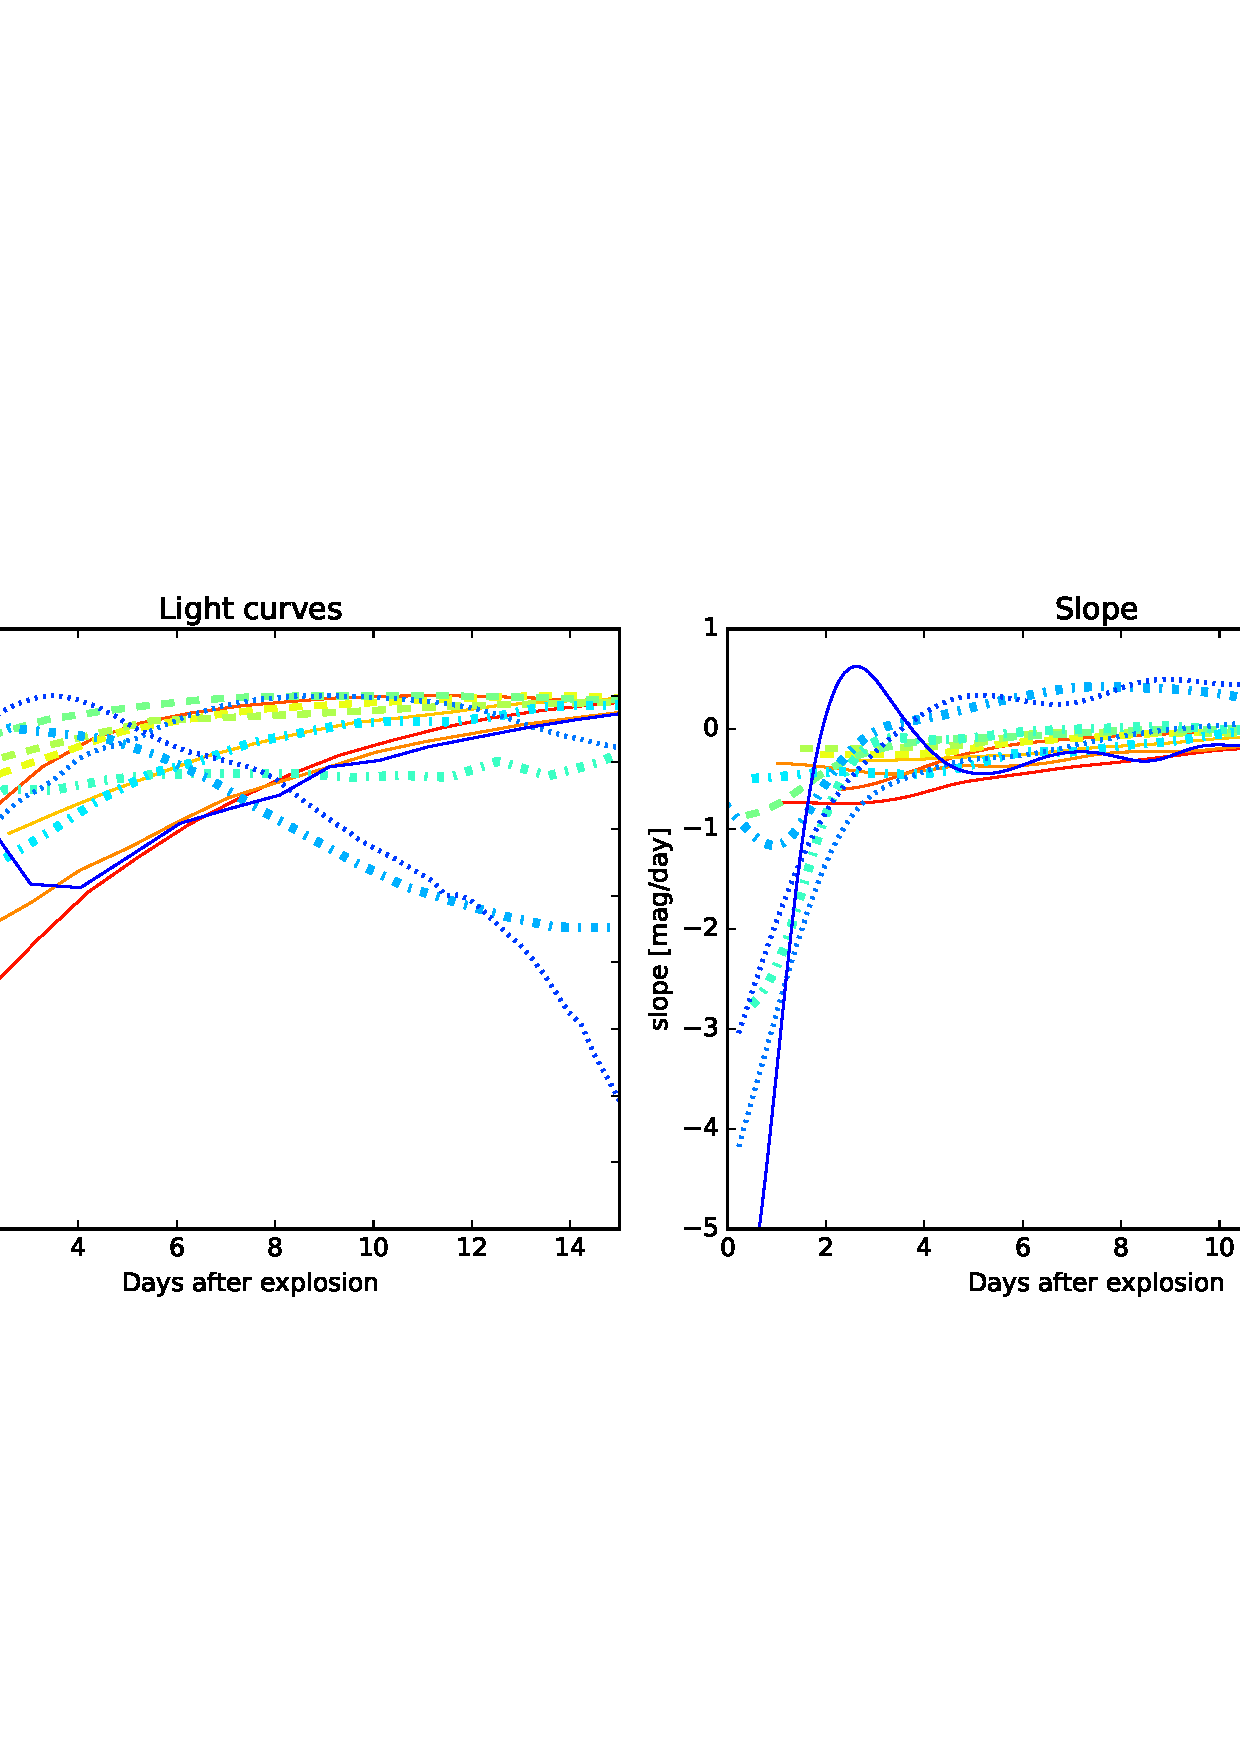
\includegraphics[width=\textwidth]{figs/transients/earlyslope1.pdf}
}
\caption{\emph{Left}: $r'$-band light curve for representative transients as function of the phase from the beginning of the transient outburst/explosion for the first few days of the transient life. \emph{Right}: slope of the transient evolution. Data from: SN~Ia,~\citet{Olling15}; SNII,~\citet{Rubin16}; SN~.Ia,~\citet{Shen10}; SN~Ib,~\citet{Valenti11},~\citet{Cao13}; SN~Ic,~\citet{Mazzali02}; CV, ~\citet{Sokoloski13}, Finzell et al. (in prep), SN~Ia+interaction (see~\autoref{sec:\chpname:SNtransients})}.
\label{fig:earlyslope}
\end{figure}

\begin{figure}[hbt]
\centerline{
\includegraphics[width=\textwidth]{figs/transients/earlyrise1.pdf}
}
\caption{Observed magnitude change between two consecutive observations for a representative set of astronomical transients, as a function of the phase. We consider observation gaps of 30 minutes  (left panel), 2 hours (central panel) and 24 hours (right panel).
}
\label{fig:earlyrise}
\end{figure}
\begin{figure}[hbt]
\centerline{
\includegraphics[width=\textwidth]{figs/transients/TransientsAgeSimilarity.png}
}
\caption{Similarity matrix of transients in \autoref{fig:earlyslope} and \autoref{fig:earlyrise} for a given time gap between observations in the same filter: the similarity is measured between the rise slope of the transients. Darker color indicates a larger distance between transients.
}
\label{fig:earlyrise}
\end{figure}

% ====================================================================

 \subsection{Conclusions}

 Here we answer the ten questions posed in
 \autoref{sec:intro:evaluation:caseConclusions}:

 \begin{description}

 \item[Q1:] {\it Does the science case place any constraints on the
 tradeoff between the sky coverage and coadded depth? For example, should
 the sky coverage be maximized (to $\sim$30,000 deg$^2$, as e.g., in
 Pan-STARRS) or the number of detected galaxies (the current baseline but
 with 18,000 deg$^2$)?}

 \item[A1:] No strong constraint, as long as larger sky coverage does not compete with dense cadences
required for fast transients.

 \item[Q2:] {\it Does the science case place any constraints on the
 tradeoff between uniformity of sampling and frequency of  sampling? For
 example, a rolling cadence can provide enhanced sample rates over a part
 of the survey or the entire survey for a designated time at the cost of
 reduced sample rate the rest of the time (while maintaining the nominal
 total visit counts).}

 \item[A2:] Two visits/night is not sufficient - a rolling cadence can provide a satisfactory solution.

 \item[Q3:] {\it Does the science case place any constraints on the
 tradeoff between the single-visit depth and the number of visits
 (especially in the $u$-band where longer exposures would minimize the
 impact of the readout noise)?}

 \item[A3:] Anything that reduces the number of visits per field potentially compromises the objectives.

 \item[Q4:] {\it Does the science case place any constraints on the
 Galactic plane coverage (spatial coverage, temporal sampling, visits per
 band)?}

 \item[A4:] The requirement for multiple visits/filters per night applies to all fields.

 \item[Q5:] {\it Does the science case place any constraints on the
 fraction of observing time allocated to each band?}

 \item[A5:] No.

 \item[Q6:] {\it Does the science case place any constraints on the
 cadence for deep drilling fields?}

 \item[A6:] As discussed in detail above, short bursts of visits separated by several days is not
satisfactory - deep drilling cadences can be devised to provide excellent sampling.

 \item[Q7:] {\it Assuming two visits per night, would the science case
 benefit if they are obtained in the same band or not?}

 \item[A7:] If two visits only, different filters may be the most effective. If more than two visits, the most closely spaced pair should be in the same filter, and the other visits should include at least one other filter.

 \item[Q8:] {\it Will the case science benefit from a special cadence
 prescription during commissioning or early in the survey, such as:
 acquiring a full 10-year count of visits for a small area (either in all
 the bands or in a  selected set); a greatly enhanced cadence for a small
 area?}

 \item[A8:] A greatly enhanced cadence would provide a strong test of the methodology and would jump-start the science.

 \item[Q9:] {\it Does the science case place any constraints on the
 sampling of observing conditions (e.g., seeing, dark sky, airmass),
 possibly as a function of band, etc.?}

 \item[A9:] None unique to transients.

 \item[Q10:] {\it Does the case have science drivers that would require
 real-time exposure time optimization to obtain nearly constant
 single-visit limiting depth?}

 \item[A10:] No.

 \end{description}


% --------------------------------------------------------------------

% ====================================================================
%+
% SECTION:
%    sn.tex
%
% CHAPTER:
%    transients.tex
%
% ELEVATOR PITCH:
%
%-
% ====================================================================

\section{Supernovae as Transients}
\def\secname{\chpname:SNtransients}\label{sec:\secname}

\credit{fedhere}

Supernovae (SNe) represent the final dramatic stages of the life of many
stars. The term SN we covers a diverse set of phenomena: explosion of
low mass stars in binary systems, thermonuclear SN or SN Ia (also
discussed in \autoref{sec:supernovae}), and explosion of high mass stars,
Core collapse (CC) SNe, and even terminal explosions of more exotic
systems, yet to be understood, like Super Luminous SNe
(SLSNe). Phenomenologically, the observables of the explosion are
also diverse. The transient duration ranges between weeks,
months, even years. The electromagnetic energy radiated ranges between
$\sim0.1$ (faintest CC SNe), to $\sim1$ (SN Ia) and $\sim100$ (SLSNe)
$\times 10^{49}$ erg, corresponding to absolute magnitudes at peak
ranging between $\sim-19$ and $\sim-22$.

LSST's contribution to SNe studies can be substantial. Synoptic
surveys such as SDSS, SNLS, PTF, PanSTARRS have revolutionized our
understanding of SN time and again, exposing their diversity,
and revealing different progenitor channels. LSST's first crucial
input will be discovery: the normal type Ia SN rate out to redshift
$z=1$ is estimated to be $\sim200 ~(\mathrm{sq. deg.})^{-1}$ per
year\footnote{\url{http://www.lsst.org/sites/default/files/docs/Wood-Vasey_086.11.pdf}},
and SN~Ia represent only about 1/4 of all SN
events~\citep{Li11b}: tens of millions of stars will explode
within the LSST footprint every year. The main factors affecting 
LSST SN science concern:
\begin{enumerate}
\item
LSST's SN discovery power,
\item
LSST's discrimination power,
\item
the quality of the statistical sample over time.
\end{enumerate}
Items 1 and 2 are \emph{time sensitive}, while the latter
is not, although it is interesting to understand the pace at which a
science question can be advanced in the lifetime of LSST.

{\bf \emph{Discovery:}} the SN~Ia discovery is rate is a standard LSST time-domain metric: a
fraction of $\sim40\%$ SN~Ia $z\lesssim0.5$ are expected to be discovered pre-peak
luminosity within the standard LSST survey
(e.g. \opsimdbref{db:baseCadence}~Figure~\ref{fig:enigmaEarlySNe}). The
topic of SNe discovery is discussed in further detail in
\ref{sec:supernovae}.

The next step is then {\bf\emph{discrimination}}, and the question we need
to answer, for SNe as well as for most other transients, is: will LSST
photometry allow to distinguish SN from other transients, and to
distinguish the different types of SN? And further: will this be
achievable in time to appropriately direct follow-up efforts? This is
particularly difficult considering that photometric classification
schemes have only achieved modest performances in distinguishing, for
example, SN~Ic from SN~Ia. As mentioned earlier in this chapter, the issue
of prompt classification is at the heart of the success of LSST
transient science, but it is too complex to tackle in this chapter,
while LSST's ability to assess whether a new transient is young is discussed
in \autoref{sec:\chpname:transientsAge}.

When a large statistical sample of SNe is generated, LSST's photometry
may allow setting constraints on the diversity of the sample, even as a
standalone survey, without the aid of follow-up efforts.  {\bf Thus
  LSST \emph{alone} can shed light on the diversity within the
  population of SN}, which in turn may constrain the genesis of the
explosion.\footnote{Reliable typing of a SN and redshift determination
  would still require auxiliary data.} For SN~Ia, where the exploding
star is a carbon-oxygen White Dwarf (WD), outstanding questions
that can be answered by an LSST photometric sample include, for
example, what is the percentage of SN Ia that arise from a
\emph{double-degenerate} (DD) progenitor system -- a carbon-oxygen WD-WD binary
--, from a \emph {single-degenerate} (SD) system -- a WD-Main Sequence
 or WD-Red Giant (RG) binary--, or a \emph{merger} -- a WD-WD
 binary with a He and a carbon-oxygen WD.
 Answering this question would reduce the
scatter in the Hubble diagram if SNe from different progenitors are
shown to require different standardization~\citep{Scolnic2014}. On the
CC~SN side: the diversity of SN sub-classes, and the relationship
between them (is there a phenomenological continuum or are they actually
distinct classes, e.g. between IIp and IIL, or Ib and IIb?) is yet to
be understood. Exceptionally well-studied objects may answer these
questions: individual SN Ia with tight constraints on the progenitor
system show, for example, that both single and double degenerate
progenitors exist (e.g. SN 2011fe, \citealt{Li11}, ~\citealt{Olling15}
and PTF 11kx, \citealt{Dilday12}). However, a statistical sample is
needed to set constraints on populations~\citep{Hayden2010, Bianco11}.

Thus the technical question to be answered is: how much detail can be
sacrificed in favor of sample size without compromising diagnostic
power? And the diagnostic power relies on color and sampling: thus
what is the trade-off between cadence in the same filter, and
observations in different filters. Specifically, transients can be
distinguished early from two photometric characteristics: rise time
and color. There is a tension between these observables, as discussed
in Section~\ref{sec:\chpname:transientsAge}. Obtaining colors relies
of course on obtaining photometry in different bands as close as
possible to \emph{simultaneously}.  However, assessing the rise slope
is best done with a single filter, so prompt characterization also
needs multiple epochs within a night, although separated by at least a
few hours, in the same filter, as observing with different
filters it is impossible (or very hard) to separate shape from
color. Colors are an important diagnostic for the
statistical sample: as long as the epoch of peak is reliably assessed
coadded light curves can be studied, which is the goal of the analysis
that follows.

\subsection{Distinguishing progenitor scenarios}

In this chapter we envision and design a SN related metric that works
on a large sample (months-to-years of LSST data) and assesses the
ability to characterize the contribution of SNe with specific features
to the global population: as a test case we will use the presence of
an early blue excess for SN type Ia, signature of interaction with a
companion, and thus of a SD progenitor. Equivalently, the presence of
an early blue excess in CC~SNe could be assessed, the signature of
shock breakout which directly measures the radius of the progenitor
star. We perform the simulation on SN~Ia since statistical studies of
samples that set constraints on progenitor fractions (fraction of DD
vs SD progenitors) exist and can be used as a
benchmark~\citep{Hayden2010, Bianco11}.  What we evaluate as a
\emph{figure of merit} (FoM) for this science deviates from the
guidelines for figures of merit, since LSST will surely be able to
answer this question \emph{at some point} and we measure \emph{how
  fast} LSST can answer this question. The FoM is time
within the survey required to achieve a sufficiently large sample of
SNe to enable us to distinguish
populations with different contribution from DD and SD progenitors.
We rely on simulations of the observables of the population for
different sample sizes, and on the \texttt{transientAsciiMetric} to
determine the detectability of interacting vs non-interacting
SNe. We are developing a metric (\texttt{colorGapMetric}) to assess
the gap between of detections in 2 filters. In the meantime, we rely on
the estimated of the gap between observations in a single filter, and
in any filters (see~\autoref{sec:\chpname:analysis}).

We simulate interacting SNe from the Nugent templates \citep{Nugent02}
injecting the angle-dependent effects of interaction with a companion
as simulated by \citep{Kasen10}, for a $2~M_\odot$ and a $6~M_\odot$
MS companion stars, and a $1~M_\odot$ RG companion, following the
procedure designed in ~\citep{Bianco11}. We create synthetic progenitor
populations with a fraction of single degenerate progenitor systems
$0.05 \leq f_\mathrm{SD} \leq 0.6 $ in 0.05 intervals, and random lines of
sight with respect to the binary's geometry. One such lightcurve, with
maximal interaction effects, is shown in \autoref{fig:kasenlc}, also
indicating how it may be observed by LSST. For each population, we
simulate the observation of colors by selecting random epochs with a
granularity of 1 day within the first 10 days after explosion, and
subtracting the magnitude in different filters at the same epoch
$\pm~1$~day for each SN, and we include the effects of observational
noise by generating datapoints from a draw within a Gaussian
distribution centered at the color measured in the previous step and
with standard deviation $\sigma_\mathrm{pop} = 0.1$, 0.3, and 0.5.
The SNR requirement is
translated into a requirement on each
observation of $\mathrm{SNR} >
\frac{1.0}{\sqrt{2.0}~\sigma_\mathrm{pop}}$.
We generate populations of $N_\mathrm{pop}=100$,~1000,~10000 $z~=~0.5$ SNe,
observed in $g'-r'$, as a representative case. Because the effect is
heavily chromatic, and it dissipates becoming essentially negligible
by $r$ band, $u'-i'$ gives the most leverage. However $g'$ and $r'$
are the best observed LSST bands in most cadences. An extension of
this work should then consider $g'-r'$, $u'-r'$, $g'-i'$, and $u'-i'$.

\begin{figure}[hbt]
\centerline{
\includegraphics[width=0.6\textwidth]{figs/transients/LSST_Kasen_lcv0.pdf}
}
\caption{ A normal SN Ia lightcure at z=0.5 showing interaction with a
  RG companion as seen from the most favorable viewing angle: the
  effect of interaction as simulated by \citet{Kasen10} is added on
  top of a lightcurve simulated from the \citealt{Nugent02}
  templates. The data points represent one possible set of LSST
  observations of this transient, obtained by running the
  \texttt{transientAsciiMetric}.  This particular event is detected in
  $g'$, $r'$, and $i'$ within the first 10 days.}
\label{fig:kasenlc}
\end{figure}

We perform Kolmogorov-Smirnoff ($KS$) an Anderson-Darling ($AD$) tests
to evaluate our diagnostic power as a function of sample quality,
$SNR$, and sample size, $N_\mathrm{pop}$.  In
\autoref{tab:SNprogenitors} we report the ability to distinguish a
population with a $f_\mathrm{SD} > x$ from $f_\mathrm{SD}=0.05$; \emph{the
number reported is the SN~Ia fraction from SD progenitors that can be
distinguished at a $p\mathrm{-value}~\leq ~0.05$}.

\begin{table}
\begin{center}
  %\begin{tabular}{ c | c| c| c | c | c| c| c | }
  \begin{tabular}{ c | c| c| c |  }
$g-r$&\bf{$N_\mathrm{pop}$=100}&\bf{$N_\mathrm{pop}$=1,000}&\bf{$N_\mathrm{pop}$=10,000}\\%& $g-i$&\bf{$N$=100}&\bf{$N$=1,000}&\bf{$N$=10,000} \\
  \hline
  {\bf $\mathrm{SNR}~\geq~1.4$}&  -  & 0.2 & 0.1 \\%& &  -  & -  &  0.2 \\
  {\bf $\mathrm{SNR}~\geq~2.0$}&  - & 0.2 & 0.1 \\%& &  -  & 0.2 & 0.1 \\
  {\bf $\mathrm{SNR}~\geq~7.0$}& 0.2 & 0.1 & 0.1 \\%& & 0.4 & 0.1 & 0.1 \\
%&&&&&&&\\ $u-i$&\bf{$N$=100}&\bf{$N$=1,000}&\bf{$N$=10,000} & $u-r$&\bf{$N$=100}&\bf{$N$=1,000}&\bf{$N$=10,000}\\
% \bf{$\sigma_\mathrm{pop} = 2.0$}&  -  & -  &  0.2 & &  -  & -  &  0.2 \\
% \bf{$\sigma_\mathrm{pop} = 1.0$}&  -  & 0.2 & 0.1 & &  -  & 0.2 & 0.1 \\
% \bf{$\sigma_\mathrm{pop} = 0.5$}& 0.4 & 0.1 & 0.1 & & 0.4 & 0.1 & 0.1 \\

 \hline
  \end{tabular}
  \caption{Minimum fraction of single-degenerate (SD) SN~Ia in a sample of size $N_\mathrm{pop}$ of $z~=~0.5$ SNe that can be distinguished from a population with a fraction of 0.95 double-degenerate (DD) and 0.05 SD SNe~Ia, for a given quality cut on each observed datapoint ($\sigma_\mathrm{pop}$).}
\label{tab:SNprogenitors}
\end{center}
\end{table}

Now we can evaluate how long it will take for a given LSST
cadence to obtain a sufficient number of observations in the 2 desired
bands, separated by less than 1 day, that pass the SNR requirements.
This should be done in a full Monte Carlo simulation, injecting
light curves with the proper light curve shape at the proper rate.  Note
that, because the early light curves of interacting SD SN~Ia are
brighter, they should be more easily detected. However, at this stage we
can take some shortcuts. \emph{First shortcut}: we evaluate the
relative observability of SNe with excess, and SNe without excess at
$z~=~0.5$ and adjust the number of detections according to
the injected ratio.  The relative detectability can be assessed with
the \texttt{transientAsciiMetric}, which allows us to see how OpSims
recovers observations of transients with realistic shapes. We conclude
that for RG-WD progenitors the detectability is enhanced by $\sim50\%$ in
 $g'$ compared to SD progenitors, and slightly less in $r'$. 
Then we extract from the \texttt{transientAsciiMetric}, the number of
\emph{color observations}, i.e. observations in 2 bands within 1 day
of each other, each fulfilling our SNR requirement for the color for
3-, 6-, and 12 months of survey in year 1. 

With the goal of distinguishing a SD contribution of 10\% to the SN Ia
population from a 5\% contribution to a three-sigma level ($p$-value
$<0.05$) we need more than 1000 detections within 1 day in 2 filters
at a $\mathrm{SNR}~\geq~7$: \autoref{tab:SNprogenitors}. But the pairs
of observations we recovered in the previous steps are within the
first 10 days but with any gap in time. \emph{Second shortcut}: To
include the constraint that the detections should be within 24 hours
we use to the \texttt{InterNightGapsMetric}, which is plotted in
~\autoref{fig:enigmaGapAll}.  For the \opsimdbref{db:baseCadence} we
estimate $~\sim10\%$ of the observation are revisited within a
night. With the assumption that this is likely to happen in two
different filters, which is \emph{non-conservative}, but neglecting
intra-night observations that may happen in the two different filters,
which is a \emph{conservative} assumption our numbers drop by a factor
10. The lightcurves are injected with an event rate designed to be
consistent with the discovery rate measured in \ref{sec:supernovae}.

With all these assumptions standing, we find that that only 3 months
of survey are sufficient to provide a sufficiently large and
sufficiently high SNR sample for our purpose, and improve on the
findings on this topic that were achieved with
SDSS~II~\citep{Hayden2010}, and 3 years of SNLS data~\citep{Bianco11}
with \opsimdbref{db:baseCadence} or the
\opsimdbref{db:NEOswithVisitTriplets}. The
\opsimdbref{db:NEOswithVisitTriplets} requires three visits, thus
increasing the timeline for inter-night observations. Although it does not
require the observations to be in any specific filters, and with the
addition of the third visit within the same night, it increases the
typical intra-night gap, it outperforms \opsimdbref{db:baseCadence} slightly.
It is possible that a detailed investigation
of the true \emph{inter-night gap between different filters}, or the
addition of a requirement in the cadence that one of the night filters
be different than the others (possibly requiring an increased gap
between two of the three images to minimize filter changes) would
provide valuable data for this kind of studies even faster.

\emph{This exercise demonstrates the power of LSST in collecting large high SNR samples of transients, but we must remind the reader that these conclusions, and generally large sample analysis, rely on having properly identified both the transient class (normal SN~Ia) and the date of maximum! This, once more, highlights the importance of prompt identification and classification: for SN~Ia this likely will limit this work to objects that could be identified spectroscopically, enhancing the importance of follow-up.}


\autoref{fig:sndetect} shows the detection rate for SN~Ia at $z=0.5$
in absence of shock interaction as a function of SNR (obtained by summing in quadrature the errors on $g'$
and $r'$) for 3, 6 months, and a year of
\opsimdbref{db:baseCadence} and \opsimdbref{db:NEOswithVisitTriplets}.
% (ideally I will plot it for the other survey as well tonight)



\begin{table}
  \begin{tabular}{l|p{8cm}|c|c|p{3cm}}
    FoM & Brief description & {\rotatebox{90}{\opsimdbref{db:baseCadence}}}
	  & {\rotatebox{90}{\opsimdbref{db:NEOswithVisitTriplets}}} & Notes \\
    \hline
    \thesection-1 & \footnotesize{\texttt{SNIaprojenitorMetric},
    \nolinebreak{\texttt{1,000 detections}}}      & 3 & $<3$ &
    \footnotesize{Time in month to collect 1,000 relevant observations to distinguish a 5\% from a 10\% SD contribution} \\
    \thesection-2     & \footnotesize{\texttt{SNIaprojenitorMetric},
    \texttt{10,000 detections}}      & $>12$ & $>12$ &
    \footnotesize{Time in month to collect 10,000 relevant observations in months  to distinguish a 5\% from a 10\% SD contribution.}\\
\end{tabular}
\caption{FoMs for statistical SN Ia progenitor studies to assess the contribution of SD progenitors to the SN Ia population.
}
\label{tab:SummarySNprojs}
\end{table}

\begin{figure}[hbt]
  \centerline{
    \includegraphics[width=0.6\textwidth]{figs/transients/LSST_Iadetected_wcolor.png}
  }
  \caption{
    Normal SN Ia light cure at z=0.5 detected by the \opsimdbref{db:baseCadence} (solid lines) and \opsimdbref{db:NEOswithVisitTriplets} cadence (dashed line) in 3 months, 6 months, and 1 year, that provide color information useful to constrain the progenitor distribution. Line are third-degree polynomial fits.}
  \label{fig:sndetect}
\end{figure}

% ====================================================================
%
 \subsection{Conclusions}

 Here we answer the ten questions posed in
 \autoref{sec:intro:evaluation:caseConclusions}:

 \begin{description}

 \item[Q1:] {\it Does the science case place any constraints on the
 tradeoff between the sky coverage and coadded depth? For example, should
 the sky coverage be maximized (to $\sim$30,000 deg$^2$, as e.g., in
 Pan-STARRS) or the number of detected galaxies (the current baseline but
 with 18,000 deg$^2$)?}

 \item[A1:] Yes, although this question can be answered with a full simulation that includes a coordinate dependent event rate while the current simulation assumes uniform probability of a transient in the field-of-view and cannot evaluate this trade-off

 \item[Q2:] {\it Does the science case place any constraints on the
 tradeoff between uniformity of sampling and frequency of sampling? For
 example, a rolling cadence can provide enhanced sample rates over a part
 of the survey or the entire survey for a designated time at the cost of
 reduced sample rate the rest of the time (while maintaining the nominal
 total visit counts).}

 \item[A2:] Yes: this science case is sensitive to both. A more sophisticated simulation which also measures the ability to correctly identify the epoch of maximum would be more powerful to answer the question.
   

 \item[Q3:] {\it Does the science case place any constraints on the
 tradeoff between the single-visit depth and the number of visits
 (especially in the $u$-band where longer exposures would minimize the
 impact of the readout noise)?}

 \item[A3:] Yes, because the diagnostic power depends on both the SNR of each observation and the gap between observations. 

 \item[Q4:] {\it Does the science case place any constraints on the
 Galactic plane coverage (spatial coverage, temporal sampling, visits per
 band)?}

 \item[A4:] No.

 \item[Q5:] {\it Does the science case place any constraints on the
 fraction of observing time allocated to each band?}

 \item[A5:] Yes, since it relies on obtaining observations in at least 2 filters.

 \item[Q6:] {\it Does the science case place any constraints on the
 cadence for deep drilling fields?}

 \item[A6:] Yes, although the results have not been analyzed separately for WFD and DD fields.

 \item[Q7:] {\it Assuming two visits per night, would the science case
 benefit if they are obtained in the same band or not?}

 \item[A7:] No. Although  we would benefit greatly from 2 visits in the same filters, and one visit in a different filter to constrain simultaneously shape and color."

 \item[Q8:] {\it Will the case science benefit from a special cadence
 prescription during commissioning or early in the survey, such as:
 acquiring a full 10-year count of visits for a small area (either in all
 the bands or in a  selected set); a greatly enhanced cadence for a small
 area?}

 \item[A8:] A full event rate needs to be inculded in the simulation to answer this question.

 \item[Q9:] {\it Does the science case place any constraints on the
 sampling of observing conditions (e.g., seeing, dark sky, airmass),
 possibly as a function of band, etc.?}

 \item[A9:] Yes since detection depends on SNR.

 \item[Q10:] {\it Does the case have science drivers that would require
 real-time exposure time optimization to obtain nearly constant
 single-visit limiting depth?}

 \item[A10:] No.

 \end{description}


% --------------------------------------------------------------------

% ====================================================================
%+
% SECTION:
%    grb.tex
%
% CHAPTER:
%    transients.tex
%
% ELEVATOR PITCH:
%-
% ====================================================================

\section{Gamma-Ray Burst Afterglows}
\def\secname{grbs}\label{sec:\secname}

\credit{ebellm}

Gamma-ray bursts (GRBs) are relativistic explosions typically classified
by the temporal duration of their initial gamma-ray emission: Long GRBs,
that mark the endpoint of the lives of some massive stars, and short
GRBs, believed to originate from the merger of binary neutron stars. GRB
emission is known to be beamed: the initial prompt gamma-ray emission is
seen only for observers looking at the jet axis. The longer-wavelength
X-ray, optical, and radio afterglow may be seen both by on- and off-axis
observers.  The latter case is known as an orphan afterglow, due to the
absence of gamma-ray emission. On- and off-axis afterglows are predicted
to have different temporal signatures in the optical: On-axis events
decay as a power-law until a jet break, while off-axis events should be
fainter and show an initial rise (Figure \ref{fig:afterglow_lcs}).
Despite systematic searches, no convincing orphan afterglow candidates
have yet been discovered, limiting our knowledge of the beaming fraction
of GRBs and hence their true rates. Well-sampled orphan afterglow
lightcurves would also permit study of the GRB jet structure.

\begin{figure}[hbt]
\centerline{
\includegraphics[width=0.6\textwidth]{figs/transients/predicted_afterglow_lcs_mag.pdf}
}
\caption{ Predicted light curves of GRB afterglows by off-axis angle
with respect to the jet axis $\theta_{\rm obs}$ \citep[Figure
8.8,][]{2009arXiv0912.0201L}. The forward shock model is derived from
\citet{2002ApJ...576..120T} and assumes a jet half opening angle
$\theta_j = 4^\circ$, the isotropic equivalent energy of $E_{\rm iso} =
5\times10^{53} \rm erg$, ambient medium density $n = 1$ g cm$^{-3}$, and
the slope of the electron energy distribution $\rm p = 2.1$. The
apparent AB $r$-band magnitudes assume a source redshift $z = 1$. }
\label{fig:afterglow_lcs}
\end{figure}

Because of their rarity, in all but one case \citep{2015ApJ...803L..24C}
to date GRBs have been discovered using their prompt emission by hard
X-ray or gamma-ray all-sky monitors. This selection imposes biases on
the population of relativistic explosions we observe. Baryon-loading in
the GRB jet---a ``dirty fireball'' \citep{2003ApJ...591.1097R}---can
lead to on-axis events without gamma-ray emission.  Only one plausible
candidate has been identified to date \citep{2013ApJ...769..130C}.
Discovery of new dirty fireballs---if distinguished from off-axis
events--would clarify the rates of these events and enhance our
understanding of the diversity of stellar death.

LSST is the survey most capable of resolving these decades-old
questions.  Due to its large aperture and etendue, LSST can detect
faint, fast-fading, and rare cosmological events, potentially enabling
population studies of the high-redshift universe.
\citet{2015A&A...578A..71G} estimated LSST could detect 50 orphan
afterglows each year, more than any other planned survey.

%deep survey helps due to time dilation

%beaming fraction and true rates; jet structure; dirty fireballs?
%GRB-SN connection; probe high-z star formation?

%other fast transients: Fast transients and SN shock breakout?  flash spectroscopy

The challenge of detecting and recognizing GRB afterglows in the LSST data in
real time makes this science case a useful proxy for other fast transient
science cases that benefit from $N > 2$ visits per night.  In particular, this
includes discovering supernovae soon after explosion for flash spectroscopy or
shock breakout searches.

% need appropriate cadences to support value of realtime alert stream

% --------------------------------------------------------------------

\subsection{Target measurements and discoveries}
\label{sec:\secname:targets}

GRB afterglow discovery is among the science cases that places the
greatest stress on the LSST cadence.  Because afterglows fade
rapidly---dropping several magnitudes in the first few hours---high
cadence observations are required to detect the fast fading. If an
afterglow candidate can be recognized in real time, it will be possible
to trigger TOO spectroscopy (to measure a redshift and confirm the event
is cosmological), X-ray and radio observations (to detect a high-energy
counterpart and the presence of a jet), and additional photometry (to
characterize the lightcurve evolution).  If there is no source at the
location of the transient in the coadded reference image, two
consecutive observations in the same filter separated by an hour or two
are the minimum required to potentially trigger followup of a
fast-fading event. However, a third observation within a night or
two---ideally in the same filter---would improve the purity of the
sample and reduce the reliance on triggered followup. Observations in
other bands at high cadence are less useful because they require
assumptions about the event's SED and its evolution to determine if a
source is truly fading.

Distinguishing orphan afterglows from on-axis events (whether conventional
GRBs or dirty fireballs) will also require more than two detections.
Orphan events may prove harder to recognize in real time, because they are
intrinsically fainter than on-axis events and show an initial rise rather
than a rapid decay (Figure \ref{fig:afterglow_lcs}).  Additionally, because
of relativistic time dilation, high redshift events are easier to detect,
but these events will be fainter and more difficult to follow up.
Accordingly, population studies of orphan afterglow candidates may by
necessity be conducted with LSST photometry alone.  Such studies may only
be productive if LSST has sufficiently frequent revisits to a field in a
single filter.

% --------------------------------------------------------------------

\subsection{Metrics}
\label{sec:\secname:metrics}

The core figure of merit for GRB afterglows is simply the raw number of
on- and off-axis events detectable in two, three, or more observations,
preferably in a single filter.

The appropriate way to derive these detections is to conduct a Monte
Carlo simulation of a cosmological population of GRBs and fold it
through the LSST observing cadence \citep[cf.][]{2011PASP..123.1034J}.
We are developing this infrastructure for the MAF framework.

In the meantime, simplified metrics can give us a general idea of how well
a given cadence can characterize fast-evolving transients such as GRBs.  We
have created a new metric, \texttt{GRBTransientMetric}, that replaces the
linearly rising and decaying lightcurve in \texttt{TransientMetric} with
the $F \sim t^{-\alpha}$ decay characteristic of on-axis afterglows.  (For
the time being, we neglect the jet break that steepens the rate of decay;
this implies that our detectability estimates are optimistic.)

We simulate random on-axis afterglows using the parameters of
\citet{2011PASP..123.1034J}: the R-band apparent magnitude at 1 minute
after explosion is randomly drawn from a Gaussian with $\mu=15.35$,
$\sigma=1.59$ and decays with $\alpha=1.0$.  For these estimates we
simply assume zero color difference between in all LSST bands.
There are roughly 300 on-axis GRBs per year with these parameters;
we calculate the average fraction of these events which have at least one,
two, or three detections in any single filter.

% Can use https://github.com/lsst/sims_maf/blob/master/python/lsst/sims/maf/metrics/tgaps.py or https://github.com/lsst/sims_maf/blob/master/python/lsst/sims/maf/metrics/cadenceMetrics.py (Inter/Intra-night) to get histograms.  Would be nice to extend to single-band, N-offset

% --------------------------------------------------------------------

\subsection{OpSim Analysis}
\label{sec:\secname:analysis}

We ran \texttt{GRBTransientMetric} on several OpSim v3.3.5 runs with a range of
characteristics:  \opsimdbref{db:baseCadence}, the baseline cadence;
\opsimdbref{db:NEOswithVisitTriplets}, with three visits per WFD field;
\opsimdbref{db:NoVisitPairs}, with no visit pairs; and
\opsimdbref{db:opstwoPS}, a PanSTARRS-like cadence.

\autoref{tab:SummaryGRBs} lists the fraction of on-axis afterglows
detected in at least one, two, and three visits in a single filter.

Because of its wider areal coverage, the PanSTARRS-like cadence of
\opsimdbref{db:opstwoPS} maximizes the fraction of events detected in
one and two epochs.  Not surprisingly, the triplet-visit WFD cadence of
\opsimdbref{db:NEOswithVisitTriplets} maximizes the three-epoch detection
rate.


\begin{table}
  \begin{tabular}{l|p{6cm}|c|c|c|c|p{5cm}}
    FoM & Brief description & {\rotatebox{90}{\opsimdbref{db:baseCadence}}}
	  & {\rotatebox{90}{\opsimdbref{db:NEOswithVisitTriplets}}} &
	  {\rotatebox{90}{\opsimdbref{db:NoVisitPairs}}} &
	  {\rotatebox{90}{\opsimdbref{db:opstwoPS}}} & Notes \\
    \hline
    \thesection-1 & \footnotesize{\texttt{GRBTransientMetric},
    \texttt{nPerFilter}\,$=1$}      & 0.17 & 0.16 & 0.20 & \textbf{0.21} &
    \footnotesize{Fraction of GRB-like transients detected in at least one
    epoch.} \\
    \thesection-2     & \footnotesize{\texttt{GRBTransientMetric},
    \texttt{nPerFilter}\,$=2$}      & 0.12 & 0.10 & 0.09 & \textbf{0.14} &
    \footnotesize{Fraction of GRB-like transients detected in at least two
    epochs in any single filter.} \\
    \thesection-3     & \footnotesize{\texttt{GRBTransientMetric},
    \texttt{nPerFilter}\,$=3$}      & 0.05 & \textbf{0.08} & 0.04 & 0.04 &
    \footnotesize{Fraction of GRB-like transients detected in at least
	    three epochs in any single filter.}
\end{tabular}
\caption{Mean figures-of-merit (FoMs) for on-axis Gamma-Ray Bursts for one,
two, and three detections in a filter.
The best value of each FoM is indicated in bold.
The wider areal coverage of \opsimdbref{db:opstwoPS} improves its detection
rate of GRBs in one and two epochs, while the triplet visits
in \opsimdbref{db:NEOswithVisitTriplets} naturally improve the
three-detection efficiency.
}
\label{tab:SummaryGRBs}
\end{table}

% --------------------------------------------------------------------

\subsection{Discussion}
\label{sec:\secname:discussion}

An LSST cadence purely designed for discovering GRB afterglows would
include three or more visits to each field every night, with the visits
separated by an hour or two. Moreover, it would be conducted in a single
filter in order to best identify the lightcurve shape of off-axis
events.

While the current surveys simulated are far from this ideal
(usually just two closely spaced visits, with subsequent revisits days
later), nonetheless an appreciable number of GRBs are detectable.
\opsimdbref{db:NEOswithVisitTriplets} would detect about 25 events each
year in three epochs, already potentially the largest sample of untriggered
afterglows.

However, some care is required in interpreting these values:
while the GRB afterglow fades rapidly over the first day of the explosion
(Figure \ref{fig:afterglow_lcs}), at later times a 30 minute visit
separation is not enough to reveal significant evolution in the lightcurve.
We intend to enhance our metric to require that detections are counted only
if significant evolution is statistically distinguishable with 1\%
photometry.

In future work we intend to simulate cosmological populations of on- and
off-axis in order to better determine how many events could be discovered
in time to trigger real-time followup.

\begin{figure}[hbt]
\centerline{
\includegraphics[width=0.6\textwidth]{figs/transients/afterglow_cdf.png}
}
\caption{ Cumulative fraction of GRB on-axis afterglows fainter than
magnitude 24.7 at a given time after the burst. We use an $\alpha=1$
decay with no jet breaks and the brightness parameters of
\citet{2011PASP..123.1034J}. }
\label{fig:afterglow_visibility}
\end{figure}

Thanks to LSST's depth, GRBs can be visible for weeks (Figure
\ref{fig:afterglow_visibility}).  Accordingly,
modest enhancements to the intra- and inter-night revisit rate with
single-filter rolling cadences should substantially improve LSST's
discovery and characterization of relativistic explosions.


% ====================================================================

\navigationbar


% --------------------------------------------------------------------

% PJM: moved to Future Work while MAF analysis is pending:
% % ====================================================================
%+
% SECTION:
%    tde.tex
%
% CHAPTER:
%    transients.tex
%
% ELEVATOR PITCH:
%    Tidal disruption events (TDEs) are the disruptions of stars by supermassive black holes.
%    They can produce flares in the optical and UV (sometimes accompanied by X-ray and radio emission as well).
%    These flares can be used to reveal the properties of otherwise quiescent SMBHs and to study accretion physics.
%    TDEs are rare, LSST will allow the first statistical sample of such events.
%
% AUTHORS:
%    Iair Arcavi (@arcavi)
%
% ====================================================================

% \section{Tidal Disruption Events}
\subsection{Tidal Disruption Events}
\def\secname{\chpname:tdes}\label{sec:\secname}

\credit{arcavi}

A star passing close to a supermassive black hole (SMBH;
$M\gtrsim10^{6}M_{\odot}$) will be torn apart by tidal forces. For
certain ($\lesssim10^{8}M_{\odot}$) black hole masses, the disruption
will occur outside the event horizon and will be accompanied by an
observable flare \citep{Hills1975, Rees1988}. Such flares can be used to
study inactive SMBHs, which are otherwise inaccessible beyond the nearby
($\lesssim100$ Mpc) universe.

We are now building our understanding of how observational properties of
TDEs are affected by the SMBH. Theory claims to provide such a
connection \citep[e.g.][]{Lodato2009, Guillochon2014}, but uncertainties
in the physics of the disruption, subsequent accretion and emission
mechanisms are currently topics of debate \citep[e.g.][]{Strubbe2015,
Guillochon2014, Roth2015}, and new models are vigorously being developed
\citep[e.g.][]{Piran2015, Hayasaki2015, Svirski2015, Bonnerot2015}.

TDEs are rare ($\sim10^{-5}-10^{-4}$ events per galaxy per year;
\citealp{Wang2004, Stone2015}), and until recently, TDE candidates were
discovered mostly in archival data \citep[e.g.][]{Donley2002,
Gezari2006, Esquej2007}. Now, however, wide-field transient surveys have
started discovering TDEs in real time.

Generally, two types of TDE candidates have been identified:
\begin{enumerate}
	\item \textit{High energy TDEs}. The prototype is Swift J1644
\citep{Bloom2011, Burrows2011, Levan2011, Zauderer2011}, with two other
events known \citep{Cenko2012, Brown2015}. These events display emission
in $\gamma$-rays and X-rays as well as in the radio, but are not
detected in the optical.
\item \textit{Optical-UV TDEs}.  The prototype is PS1-10jh
(Figure \ref{fig:tde}; \citealp{Gezari2012}).
		About $8$ other events are known
\citep{Chornock2014, Arcavi2014, Holoien2014, Holoien2015, Holoien2016}.
Some events were detected also in the X-rays and radio (in addition to
the optical and UV), but the X-ray and radio signatures are different
than those of the high energy TDE candidates.
\end{enumerate}

\begin{figure}[hbt]
\centerline{
\includegraphics[width=0.6\textwidth]{figs/transients/tdeGezari.pdf}
}
\caption{
Optical and near-UV lightcurve of the TDE PS1-10jh \citep{Gezari2012}.
}
\label{fig:tde}
\end{figure}

It is still not clear whether both of these classes of transients are TDEs,
and if so, why they are so different form each other. One option raised is
that some TDEs may launch jets, which when directed towards us, appear as
the high energy events, but otherwise appear as the optical-UV events.
It is still not clear if this is indeed the case \citep[e.g.][]{VanVelzen2013}.

Here we focus on the second type of TDE candidates, which is the
relevant class for LSST, since they can be discovered in the optical.
However, multi-wavelength coordinated observations of
optically-discovered events are required in order to better understand
the connection between the two types of candidates.

The first well-sampled TDE of the optical+UV class was PS1-10jh (discovered by Pan-STARRS;
\citealt{Gezari2012}). \citet{Arcavi2014} later presented three new TDE candidates
from PTF and one discovered by ASAS-SN, all with similar properties
as PS1-10jh. These events exhibit blue colors, broad light curves,
peak absolute magnitudes of $\sim-20$ and a $\sim t^{-5/3}$ decay
at late times. This decay law has been suggested as a unique signature
of accretion-powered TDE light curves \citep{Rees1988, Evans1989, Phinney1989}.
Early-time deviations from the $t^{-5/3}$ rate
can be used to constrain the density profile of the disrupted star
\citep{Lodato2009, Gezari2012}. Late-time deviations would
test the accretion power-source hypothesis altogether.

The spectral signatures of these TDEs are still a puzzle. PS1-10jh displayed
only He II emission lines, lacking any signs of H. Some of the \citet{Arcavi2014}
sample, however, do display H emission.
In fact, a continuum of H / He emission ratios for this class of transients
is being revealed, and is now a focus of theoretical modelling \citep{Strubbe2015, Roth2015}.

The second recent discovery relating to this new sample concerns their
host galaxies \citep{Arcavi2014, French2016}, most of which are
post-starburst galaxies. These galaxies show little or no signs of on-going star formation, but their significant A stellar populations indicate that star formation ceased abruptly a few hundred Myr to a Gyr ago \citep{Dressler1983}. Galaxies with these characteristics often show signs of recent galaxy-galaxy mergers \citep{Zabludoff1996}, which produced the starburst and evolved the bulge. Optical-UV TDEs are intrinsically over abundant in post-starburst galaxies by a factor of $\sim30-200$ (depending on the characteristics of the galaxy; \citealt{French2016}). The reason for the strong preference of TDEs for post-starburst galaxies has still not been determined.

LSST's contribution to TDE studies will be substantial.
\citet{VanVelzen2011} estimate that LSST could discover approximately
4000 TDEs per year. The main drivers for studying TDEs with LSST are:
\begin{itemize}
\item Measuring black hole masses: This involves fitting models to TDE
light curves. It is also relevant to correlate these measurements with
host galaxy properties (mass, bulge/disk decomposition).
\item Constraining galactic dynamics by measuring the TDE rates as
functions of black hole mass and galaxy types.
\item Characterizing TDE emission signatures.
\end{itemize}

A metric is required for measuring how well TDEs can be identified and
distinguished from supernovae and active galactic nuclei. In general, we
expect TDEs to:
\begin{itemize}
\item Be located in the center of their host.
\item Display approximately constant blue (few $10^4$K) colors.
\item Evolve slowly (weeks-months).
\item Not show past AGN-like variability.
\item Preferentially peak around mag -20.
\item Preferentially be hosted in a post-starburst galaxy.
\end{itemize}
These criteria are based on our current knowledge of optical TDEs, which
is still in its early stages. The field is rapidly evolving, and it is
possible that new observations will change the current picture of TDE
emission. This metric is probably best combined with those discussed in
 \autoref{sec:\chpname:SNtransients} for identifying supernovae, though the
luminosity function of TDEs (or what constitutes a ``typical'' TDE light
curve) is not yet known.

A second metric is required to asses the accuracy with which the black
hole mass can be constrained from the TDE light curves. This metric can
be based on existing theoretical models to fit simulated TDE light
curves (such as TDEFit; \citealt{Guillochon2014}).

% ====================================================================
%
 \subsection{Conclusions}

 Here we answer the ten questions posed in
 \autoref{sec:intro:evaluation:caseConclusions}:

 \begin{description}

 \item[Q1:] {\it Does the science case place any constraints on the
 tradeoff between the sky coverage and coadded depth? For example, should
 the sky coverage be maximized (to $\sim$30,000 deg$^2$, as e.g., in
 Pan-STARRS) or the number of detected galaxies (the current baseline
 of 18,000 deg$^2$)?}

 \item[A1:] The number of events discovered will be approximately proportional to the sky area surveyed, multiplied by the
 average length of coverage, so added sky area is beneficial, as long as the observing season per field is not shortened.

 \item[Q2:] {\it Does the science case place any constraints on the
 tradeoff between uniformity of sampling and frequency of  sampling? For
 example, a rolling cadence can provide enhanced sample rates over a part
 of the survey or the entire survey for a designated time at the cost of
 reduced sample rate the rest of the time (while maintaining the nominal
 total visit counts).}

 \item[A2:] Uniform sampling is optimum.

 \item[Q3:] {\it Does the science case place any constraints on the
 tradeoff between the single-visit depth and the number of visits
 (especially in the $u$-band where longer exposures would minimize the
 impact of the readout noise)?}

 \item[A3:] No, as long as all filters are well represented.

 \item[Q4:] {\it Does the science case place any constraints on the
 Galactic plane coverage (spatial coverage, temporal sampling, visits per
 band)?}

 \item[A4:] This science will be accomplished away from the galactic plane.

 \item[Q5:] {\it Does the science case place any constraints on the
 fraction of observing time allocated to each band?}

 \item[A5:] Increased $u$-filter cadence valuable for TDE.

 \item[Q6:] {\it Does the science case place any constraints on the
 cadence for deep drilling fields?}

 \item[A6:] Only cadences that sample timescales of weeks and greater will be useful.

 \item[Q7:] {\it Assuming two visits per night, would the science case
 benefit if they are obtained in the same band or not?}

 \item[A7:] Different bands would be strongly preferred.

 \item[Q8:] {\it Will the case science benefit from a special cadence
 prescription during commissioning or early in the survey, such as:
 acquiring a full 10-year count of visits for a small area (either in all
 the bands or in a  selected set); a greatly enhanced cadence for a small
 area?}

 \item[A8:] A sparse cadence applied to a large sky area would be scientifically productive, but this is not a strong constraint.

 \item[Q9:] {\it Does the science case place any constraints on the
 sampling of observing conditions (e.g., seeing, dark sky, airmass),
 possibly as a function of band, etc.?}

 \item[A9:] No.

 \item[Q10:] {\it Does the case have science drivers that would require
 real-time exposure time optimization to obtain nearly constant
 single-visit limiting depth?}

 \item[A10:] No.

 \end{description}

 \navigationbar


% --------------------------------------------------------------------

% PJM: moved to Future Work while MAF analysis is pending:
% % ====================================================================
%+
% SECTION:
%    cv.tex
%
% CHAPTER:
%    transients.tex
%
% ELEVATOR PITCH:
%    Explain in a few sentences what the relevant discovery or
%    measurement is going to be discussed, and what will be important
%    about it. This is for the browsing reader to get a quick feel
%    for what this section is about.
%
% AUTHORS:
%    Federica Bianco (@fedhere)
%
% ====================================================================

% \section{Cataclismic Variables}
\subsection{Cataclismic Variables}
\def\secname{\chpname:CVtransients}\label{sec:\secname}

\credit{paulaszkody},
\credit{fedhere}

Cataclysmic Variables (CVs) encompass a broad group of objects
including novae, dwarf novae, novalikes, and AM CVn systems, all with different
amplitudes and rate of variability. The one thing they all have in
common is active mass transfer from a late type companion to a
white dwarf. These create variability on a wide range of timescales:

\begin{itemize}
	\item \textit{minutes} flickering in
dwarf novae and novalikes, pulsations in accreting white dwarfs in
the instability strip, orbital periods of AM CVn systems
\item \textit{hours} orbital periods of novae, dwarf novae and novalikes
\item \textit{days} normal outburst lengths of dwarf novae
\item \textit{weeks} outburst length of superoutbursts in short orbital period
dwarf novae, outburst recurrence time of normal outbursts in short
orbital period dwarf novae
\item \textit{months} outburst recurrence time of
longer period dwarf novae, various state changes in novalikes, declines
in novae
\item \textit{years} for the outburst recurrence timescales of the
shortest period dwarf novae and the recurrence times in recurrent novae
\end{itemize}
The
amplitudes range from tenths of mags for flickering and pulsations to 4 mags
for normal dwarf novae and changes in novalike states up to 9-15 mags for the
largest amplitude dwarf novae and classical novae.

These large differences make correct classification with LSST difficult
but necessary in order to reach goals of assessing the correct number
of types of objects for population studies of the end points of
binary evolution. Multiple filters (especially the blue $u$ and $g$)
along with amplitude and recurrence of variation provide the best
discrimination, as all CVs are bluer during outburst and high states of
accretion. Long term, evenly sampled observations can provide indications
of the low amplitude random variability and catch some of the more frequent
outbursts, but higher sampling is needed to determine whether an object
has a normal or superoutburst, to catch a rise to outburst or to a
different accretion state or to follow a nova. Novae typically
have rise times of a few days, while the decline time and shape provide
information as to the mass, distance and composition. The time to decline
by 2-3 magnitudes is correlated with composition,
%
% FED: what is a range of time scales for this decline? days? months?
%
WD mass and location in
the galaxy, thus enabling a study of Galactic chemical evolution.  As with SN,
the diagnostic power for all these systems rests on color and sampling.

Metrics to be developed would assess the abilities of  a given observing
strategy to distinguish between new novae and dwarf novae outbursts and
identify high and low states.  This discriminiation is provided by
measurement of the shapes and recurrence times of large variations as well
as blue colors to distinguish low amplitude variability that would indicate
new pulsators or novalikes. Population studies rely on the numbers of long
orbital period (low amplitude, wide outbursts) vs. short orbital period
(patterns of short outbursts followed by larger, longer superoutbursts)
dwarf novae at different places in the galaxy, as well as the numbers of
recurrent (1-10 yrs) vs. normal novae (10,000 yrs, about 35/galaxy/yr).
Objects particulary worthy of later followup are containing highly magnetic
white dwarfs. These objects can be identified in a large sample when the
magnitude for a majority of the years is a faint (low) state and a small
percentage of time is a bright (high) state, combined with a red color (due
to cyclotron emission from the magnetic accretion column).

% ====================================================================
%
\subsection{Conclusions}
%
% Here we answer the ten questions posed in
% \autoref{sec:intro:evaluation:caseConclusions}:
%
 \begin{description}

 \item[Q1:] {\it Does the science case place any constraints on the
 tradeoff between the sky coverage and coadded depth? For example, should
 the sky coverage be maximized (to $\sim$30,000 deg$^2$, as e.g., in
 Pan-STARRS) or the number of detected galaxies (the current baseline
 of 18,000 deg$^2$)?}

 \item[A1:] Extending the sky area is not a priority for this science.

 \item[Q2:] {\it Does the science case place any constraints on the
 tradeoff between uniformity of sampling and frequency of  sampling? For
 example, a rolling cadence can provide enhanced sample rates over a part
 of the survey or the entire survey for a designated time at the cost of
 reduced sample rate the rest of the time (while maintaining the nominal
 total visit counts).}

 \item[A2:] Intervals of higher cadence are extremely valuable and a rolling cadence is a
satisfactory approach, subject to cadence details.

 \item[Q3:] {\it Does the science case place any constraints on the
 tradeoff between the single-visit depth and the number of visits
 (especially in the $u$-band where longer exposures would minimize the
 impact of the readout noise)?}

 \item[A3:] Increasing the number of $u$-band visits will improve the characterization of CV phenomena.

 \item[Q4:] {\it Does the science case place any constraints on the
 Galactic plane coverage (spatial coverage, temporal sampling, visits per
 band)?}

 \item[A4:] Most CVs will be detected in the galactic plane, and a long, rich series of visits is needed.

 \item[Q5:] {\it Does the science case place any constraints on the
 fraction of observing time allocated to each band?}

 \item[A5:] $u$-band is diagnostic, especially $u$-$g$.

 \item[Q6:] {\it Does the science case place any constraints on the
 cadence for deep drilling fields?}

 \item[A6:] For deep drilling in the galactic plane or for local group galaxies, the best cadences would obtain several epochs  per night in
 each filter, rather than concentrating all acquisition with a filter in a single rapid burst.

 \item[Q7:] {\it Assuming two visits per night, would the science case
 benefit if they are obtained in the same band or not?}

 \item[A7:] Same filter and different filter each offer valuable information, and a mix of these two options would be preferred
pending test of both cadences.

 \item[Q8:] {\it Will the case science benefit from a special cadence
 prescription during commissioning or early in the survey, such as:
 acquiring a full 10-year count of visits for a small area (either in all
 the bands or in a  selected set); a greatly enhanced cadence for a small
 area?}

 \item[A8:] It would be very helpful to CV studies - and many other areas of transient science - to understand variability across all timescales.
 Especially valuable would be a cadence that would cover one (cluster, rich star field) with all the timescales that will not be
strongly represented  in the main survey, starting at 15 seconds.

 \item[Q9:] {\it Does the science case place any constraints on the
 sampling of observing conditions (e.g., seeing, dark sky, airmass),
 possibly as a function of band, etc.?}

 \item[A9:] No.

 \item[Q10:] {\it Does the case have science drivers that would require
 real-time exposure time optimization to obtain nearly constant
 single-visit limiting depth?}

 \item[A10:] No.

 \end{description}

 \navigationbar


% --------------------------------------------------------------------

% PJM: moved to Future Work while MAF analysis is pending:
% % ====================================================================
%+
% SECTION:
%    eruptive.tex
%
% CHAPTER:
%    transients.tex
%
% ELEVATOR PITCH:
%-
% ====================================================================

% \section{LBVs and related non-supernova transients}
\subsection{LBVs and related non-supernova transients}
\def\secname{\chpname:LBVs}\label{sec:\secname}

\credit{nathansmith}

There is a large and diverse class of visible-wavelength transient
sources recognized in nearby galaxies that appear to be distinct from
traditional novae and supernovae (SNe), and have often been associated with
the giant eruptions of luminous blue varibles (LBV), such as the 19th
century outburst of $\eta$ Carinae.  Broadly speaking, members of this
class of transients share the common properties that they have peak
luminosities below those of most core-collapse SNe and more luminous
than novae and CVs (absolute magnitudes of roughly $-$9 to $-$15 mag).
They also have H-rich spectra (usually) with relatively narrow lines
that indicate modest bulk outflow velocities of 10$^2$ to 10$^3$ km
s$^{-1}$ (although some have exhibited small amounts of material at
faster speeds).  They tend to evolve on fairly long timescales of
weeks to years, although sometimes they exhibit a quick rise to peak
similar to SNe II-P. This group of transients has gone by many names,
such as LBV eruptions, SN impostors, Type V supernovae,
intermediate-luminosity optical (or red) transients, as well as others
that often include a physical interpretation.  For brevity, these are
often collectively referred to as ``LBVs'', although many of them may
not actually be LBVs. This may be largely for historical reasons,
since LBVs were the first of these to be recognized as a class.  Some
of the subgroups may be very different from objects like $\eta$
Carinae, however.

Observationally, these eruptions are understood to represent important
and dramatic mass-loss episodes in the lives of massive stars, based
on empirical estimates for the amount of ejected matter.  Guided
largely by nearby LBVs with resolved shells, these eruptions are
expected to instigate mass loss that is comparable to or more
important than metallicity-dependent winds of massive stars.  This
mode of mass loss, regardless of the mechanism, may be a very
important ingredient in the evolution of massive stars that is
currently not included in stellar evolution models.  Correcting this
is one of the key science drivers in trying to understand the physics
these eruptions.

An important empirical discriminant of subgroups in this class comes
from their progenitor stars.  Some are indeed seen to be very
luminous, blue supergiant stars consistent with traditional LBVs.
Some, however, have somewhat less luminous, heavily dust-obscured
progenitor stars that have been associated with either dust enshrouded
blue or red supergiants, or alternatively, with super-AGB stars of
8-10 M$_{\odot}$.  The degeneracy arises because when the objects are
fully obscured by dust, one cannot actually meaure the star's
temperature, and the bolometric luminosities of super-AGB stars
overlap with more luminous red and blue supergiants.  Unfortunately,
cases when we have strong constraints on the quiescent progenitor or
rare, and once they reach their peak luminosity, there is a great deal
of overlap in observed properties.

Theoretically, these eruptions are not understood.  There are many
ideas, but few if any confirmed mechanisms tied to observed
objects. Because of the relatively low total energy indicated by
radiative luminosities and outflow speeds, these are usually discussed
as non-terminal eruptions (although this may not always be the case;
see below).  Some previously discussed theoretical ideas involve (1)
winds driven by super-Eddington instabilities (although the root cause
for suddenly exceeding the Eddington limit remains unexplained), (2)
hydrodynamic explosions caused by deep-seated energy deposition, such
as unsteady nuclear burning, (3) accretion onto companion stars in
binary systems (degenerate or not), (4) mergers in binary and triple
systems, (5) electron-capture SNe, and (6) ``failed SNe'' associated
with a weak explosion and envelope ejection that results from black
hole formation during core collapse.  The last two are terminal events
that are less luminous and lower energy than normal SNe, and the last
3 should only occur once for a given source.  There are indeed many
cases where only one such transient has been seen at the same
position, and some cases where late-time observations suggest that no
source has survived with a luminosity comparable to its progenitor.
However, there are also several well-studied examples that indicate
repeating eruptions (multiple repeating transients, multiple nebular
shells with different ages, etc).  All these theoretical mechanisms
may lead to similar observed phenomena (weak explosions, moderate
luminosities, slow expansion, dusty aftermath). This class of objects
may represent a mixed-bag of different mechanisms that get lumped
together by default as ``other'' because they are not traditional SNe.

One recent area of great interest is that eruptive non-terminal
transients have been observed, in some cases, to precede much more
powerful explosions that are seen as Type IIn supernovae.  Even if the
pre-SN transients are not observed directly, pre-SN eruptive mass loss
is inferred based on circumstellar interaction diagnistocs of the SN.
These SN precursors have observed or inferred properties that are very
similar to LBVs and related transients.  This may suggest some link
between them, but then again, most of the LBVs and other SN impostors
have been observed for decades and have not gone SN (yet).  Being able
to distinguish which of these optical transients are SN precursors and
which are not is a major science driver.  The amount of mass lost in a
precursor eruption may dramatically alter the type of SN that is
observed.  There may also be a continuum of energies in pre-SN
outbursts, extending down to more normal classes of core-collapse SNe,
but these may often go unrecognized unless the SN ius caught very
early after explosion.

Rates for these LBV-like eruptions are very poorly constrained,
largely because most previous SN and transient searches with small
telescopes have been optimized for finding more luminous SNe in a
larger volume.  This has begun to change with recent surveys, and will
be revolutionized with LSST.  From discovered examples we have,
numbers are very roughly consistent with a volumetric rate comparable
to that of core-collapse SNe or larger, but with a large error bar.
Rates of individual subclasses are not well constrainted, and limited
information often makes classification into various subgroups
difficult or highly subjective.  The ``rate'' also depends on how
faint the lower limit of inclusions is; evidence suggests that the
brightest events are more rare, and that numbers increase as one moves
to lower luminosity.  At the faint end, it becomes difficult to
distinguish between eruptions and regular variability of LBVs, or
between massive star eruptions and CVs (unless detailed progenitor
information is avaialble).  Having deep, pre-eruption characterization
of sources at the positions of these eruptive transients (as well as
SN precursors) will likely be a major contribution of LSST.

In terms of timescales, many of the eruptive transients exhibit rise
and decline timescales similar to normal SNe~II-P or II-L, but with
fainter peak luminosity.  For these, observational cadence
requirements will be the same as SNe.  For some eruptive transients,
however, the rise timescales can be very long (rising a few magnitudes
in years).  While LSST's cadence will certainly be fast enough, being
able to discover slowly rising tranients that do not change much from
night to night will be an important metric.

For the faster-rising transients, spectroscopic followup is needed to
discriminate these from normal SNe, and also contextual information
about the host galaxy (and hence, the absolute magnitude) is needed to
differentiate these non-terminal eruptions from Type IIn supernovae
(their spectra look similar, although LBVs do tend to have narrower
lines).  Spectral and color evolution, as well as information about
the progenitor, is needed to distinguish among subgroups within the
class.  Multiwavelength followup is often extremely valuable or even
essential; i.e. mid-IR tells us if an optically invisible source is
cloaked in a dust shell but still quite luminous; Xrays and radio tell
us if an expanding shock wave is the likely source of persistent
luminosity.  For these reasons, nearby cases will continue to be the
most valuable in deciphering the physics of subclasses, whereas the
increased volume in which LSST discovers these fainter transients will
drastically improve our understanding of their rates.  Armed with both
a better understanding of their underlying physics and
characterization, as well as their rates and duty cycles, these
eruptive events can then be incorporated into stellar evolution models
and population synthesis/fedback models.

% % --------------------------------------------------------------------
%
% \subsection{Metrics}
% \label{sec:\secname:metrics}
%
% % --------------------------------------------------------------------
%
% \subsection{OpSim Analysis}
% \label{sec:\secname:analysis}
%
% % --------------------------------------------------------------------
%
% \subsection{Discussion}
% \label{sec:\secname:discussion}
%
% % ====================================================================
%
% \navigationbar


% --------------------------------------------------------------------

% ====================================================================
%+
% SECTION:
%    section-name.tex  % eg lenstimedelays.tex
%
% CHAPTER:
%    chapter.tex  % eg cosmology.tex
%
% ELEVATOR PITCH:
%    Explain in a few sentences what the relevant discovery or
%    measurement is going to be discussed, and what will be important
%    about it. This is for the browsing reader to get a quick feel
%    for what this section is about.
%
% COMMENTS:
%
%
% BUGS:
%
%
% AUTHORS:
%    Phil Marshall (@drphilmarshall)  - put your name and GitHub username here!
%-
% ====================================================================

\section{Gravitational Wave Sources}
\def\secname{gw}\label{sec:\secname}

\noindent{\it Raffaella Margutti, Z. Doctor, W. Fong, Z. Haiman, V. Kalogera, V. Trimble, B.~A. Zauderer } % (Writing team)

% This individual section will need to describe the particular
% discoveries and measurements that are being targeted in this section's
% science case. It will be helpful to think of a ``science case" as a
% ``science project" that the authors {\it actually plan to do}. Then,
% the sections can follow the tried and tested format of an observing
% proposal: a brief description of the investigation, with references,
% followed by a technical feasibility piece. This latter part will need
% to be quantified using the MAF framework, via a set of metrics that
% need to be computed for any given observing strategy to quantify its
% impact on the described science case. Ideally, these metrics would be
% combined in a well-motivated figure of merit. The section can conclude
% with a discussion of any risks that have been identified, and how
% these could be mitigated.

The first detection of Gravitational Waves (GW) by the advanced LIGO/Virgo collaboration \citep{Abbott16, Abbott09, Acernese08} has recently opened a new window of exploration into our Universe. The amount of information that can be revealed by the properties of the GW emission is immense and holds promises for revolutionary insights, including accurate masses and spins of neutron stars and black holes, tests of General Relativity and an accurate census of the neutron star (NS) and black hole (BH) populations that might challenge our current understanding of massive stellar evolution. However, GW events are poorly localized (10-100 deg$^2$ at the time of LSST operations). The identification of EM counterparts would provide precise localization and distance measurements, in addition to the necessary astrophysical context (e.g. host galaxy properties, connection to specific stellar populations) to fully exploit the revolutionary power of this new GW era.


% --------------------------------------------------------------------

\subsection{Target measurements and discoveries}
\label{sec:\secname:targets}

The first GW event was found to be associated with the merger of two black holes \citep{Abbott16,Abbott16b}. Although no EM counterpart was expected to accompany a black-hole black-hole (BBH) merger, it seems now possible that even BBH mergers  might produce short GRB-like EM emission \citep{Connaughton16, Loeb16,Zhang16,Perna16,Stone16}. Indeed, in analogy with supermassive BH mergers, shocks might develop in the just-formed circumbinary accretion disk (if a disk forms), which can produce a bright afterglow following the BBH merger (e.g. \citealt{Lippai08,Corrales10,Schnittman13}). Albeit speculative in nature, it is advisable to keep an open mind about the possibility of EM counterparts to BBH mergers. 

The most promising and better understood EM counterparts to GW events are ``kilonovae" \citep{Li98, Metzger10, Metzger12,Kasen13,Barnes13}. Kilonovae are short-lived (typical time scale of one week), apparently faint ($z\sim21$ mag at peak at 120 Mpc), red ($i-z\approx1$ mag), isotropic transients (Fig. \ref{Fig:kilonova}) due to the radioactive decay of r-process elements synthesized in the merger ejecta of a NS-NS or NS-BH system. These merging systems are the favored progenitors of short GRBs. Indeed, the signature of a kilonova emission has been recently found following the short GRB\,130603B \citep{Berger13,Tanvir13}. The key piece of information that enabled the discovery of kilonova-like emission associated with  this short GRB was its sub-arcsecond localization enabled by the detection of the optical afterglow, which allowed for an effective kilonova search with the Hubble Space Telescope (Fig. \ref{Fig:kilonova}). In contrast, the typical localization region of GW events in the LSST era is expected to be of the order of a few tens of square degrees \citep{aaa+13}. It is thus clear that the major challenges faced by the optical follow-up of GW events is represented by the combination of poor localizations with faint and fast evolving red electromagnetic counterparts.

The detection of an optical counterpart in conjunction with a GW event will significantly leverage the GW signal.
LSST, with its the wide FOV, wavelength coverage and exquisite sensitivity is uniquely poised to identify and characterize counterparts to GW events. 

\begin{figure}
\vskip -0.0 true cm
\centering
\includegraphics[scale=0.85]{figs/transients/kilonovaBerger.png}
\caption{Kilonova signature in the short GRB\,130603B as revealed by the Hubble Space Telescope (HST). The Magellan and Gemini telescopes sampled the optical afterglow of the GRB (dotted lines). The kilonova light starts to dominate the emission in the H band around a few days after the merger. Thick and dashed lines: theoretical kilonova models from \cite{Barnes13} showing that kilonovae are fast-evolving, faint and red transients. The light-curve of the SN\,2006aj associated with the long GRB\,060218  is also shown for comparison. From \cite{Berger13}.}
\label{Fig:kilonova}
\end{figure}


% --------------------------------------------------------------------



% --------------------------------------------------------------------

\subsection{OpSim Analysis and Discussion}
\label{sec:\secname:analysis}

Effective follow up of GW triggers relies on the capability to sample a relatively large portion of the sky, repeatedly, over a time scale $<1$ week, with different filters \citep{Cowperthwaite15}. In the optical band, the kilonova signature is expected to be more prominent in the $i$, $z$  and $y$ filters, which we identify as the most promising filters for the kilonova search. We emphasize however that another set of contemporaneous observations in  a ``bluer" filter is necessary to acquire color information and distinguish kilonovae from other fast-evolving transients.

We use the median inter-night gap  for visits in the same filter derived from the candidate Baseline Cadence \texttt{minion\_1016} to show that, in the absence of a Target of Opportunity (ToO) capability, it is \emph{not} possible for LSST  to play a major role in the identification of EM counterparts of GW triggers.  

To identify kilonova candidates we need at least 2 observations acquired within $\sim 1$ week  of the GW event \citep{Cowperthwaite15}.
Using the inter-night gap distribution for visits in the $y$ filter (which is the most promising filter for a kilonova search), the area of the sky covered with cadence  $\Delta t<7$ days at any given time, is $A_{sky}\sim 3000$ deg$^2$ (including deep drilling fields).  This is the area that can be searched for fast evolving transients.  Two important considerations follow:

\begin{itemize}
\item[(1)] $A_{sky}$ only covers $P\sim7$\% of the sky. The  probability that the \emph{entire} GW localization region is contained, by chance,  within $A_{sky}$ is thus very small.
\item[(2)] Even if LSST is able to cover a meaningful portion of the GW region, we would still not have color information, and we would thus be unable to filter out contaminating transients.
\end{itemize}

\textbf{We conclude that relying on the serendipitous alignment of the LSST fields with the GW localization map is not an effective strategy to follow up GW triggers and identify their EM counterparts. We thus strongly recommend a ToO capability as part of the baseline LSST operations strategy.}

Ideally, the ToO capability will allow for imaging of the GW localization map at least twice over $\Delta t\lesssim$1 week with a ``red" filter ($i$, $z$  or $y$),  and  will include the possibility to designate a desired set of filters to obtain color information. By the time of LSST operation the typical size of the GW localization region is expected to be 10-100 deg$^2$, which would require a small number of LSST re-pointings. We thus do \emph{not} anticipate a significantly disruptive impact on other LSST campaigns (especially if only the GW triggers with the best localizations in the southern sky are selected for LSST ToOs).

\textbf{At the price of re-shuffling a reasonably small number of fields, \emph{if} equipped with ToO capabilities, LSST can be the premier player in the era of EM follow up to GW sources.}






% ====================================================================

\navigationbar


% --------------------------------------------------------------------

\input{Transients/transientFuture.tex}

% ====================================================================

\chapter[MCs]{The Magellanic Clouds}
\def\chpname{mc}\label{chp:\chpname}

Chapter editors:
\credit{knutago},
\credit{dnidever}.

Contributing authors:
\credit{someoneelse},
{\it and others to follow}

% --------------------------------------------------------------------

\section{Introduction}
\label{sec:\chpname:intro}

% Introduce, with a very broad brush, this chapter's science projects,
% and why it makes sense for them to be considered together.

% This individual section will need to describe the particular
% discoveries and measurements that are being targeted in this section's
% science case. It will be helpful to think of a ``science case" as a
% ``science project" that the authors {\it actually plan to do}. Then,
% the sections can follow the tried and tested format of an observing
% proposal: a brief description of the investigation, with references,
% followed by a technical feasibility piece. This latter part will need
% to be quantified using the MAF framework, via a set of metrics that
% need to be computed for any given observing strategy to quantify its
% impact on the described science case. Ideally, these metrics would be
% combined in a well-motivated figure of merit. The section can conclude
% with a discussion of any risks that have been identified, and how
% these could be mitigated.

%A short preamble goes here. What's the context for this science
%project? Where does it fit in the big picture?

The Magellanic Clouds have always had outsized importance for
astrophysics.  They are critical steps in the cosmological distance
ladder, they are a binary galaxy system with a unique interaction
history, and they are laboratories for studying all manner of
astrophysical phenomena.  They are often used as jumping-off points
for investigations of much larger scope and scale; examples are the
searches for extragalactic supernova prompted by the explosion of
SN1987A and the dark matter searches through the technique of
gravitational microlensing.  More than 17,000 papers in the NASA ADS
include the words ``Magellanic Clouds'' in their abstracts or as part
of their keywords, highlighting their importance for a wide variety of
astronomical studies.

Our science goals are as follows:
\begin{enumerate}
\item What are the stellar and dark matter mass profiles of the
Magellanic Clouds?  Map extended disk, halo, debris, and streams.  Use
streams as probes of total mass profile.  RR Lyrae give potential for
three-dimensional stellar profile.
\item What is the satellite population of the Magellanic Clouds?
Discovery of dwarfs by DES and other surveys illuminating for
understanding distribution of dark matter subhalos and how galaxies
form in them (REFS)
\item What are the internal dynamics of the Magellanic Clouds?  Proper
motions from HST and from the ground (REFS) have measured the bulk
motions of the Clouds and have, in combination with spectroscopy,
begun to unravel the three dimensional internal dynamics of the
Clouds...
\item How do exoplanet statistics in the Magellanic Clouds compare to
those in the Milky Way?  Lund calculation shows can measure transits
of Jupiter-like planets, Clouds are lower metallicity environment
\item Identify and characterize the variable star and transient
population of the Clouds.  Population studies, linking to star
formation and chemical enrichment histories, etc, from Szkody et al.
DD white paper.
\item Light echoes from supernovae and explosive events.  Echoes can
give view of such events unavailable by any other means, ref. papers
by Rest et al.
\end{enumerate}

These goals can be categorized under two main overarching science themes:
\begin{enumerate}
\item {\bf Galaxy formation evolution}: The study of the formation and
evolution of the Large and Small Magellanic Clouds (LMC and SMC,
respectively), especially their interaction with each other and the
Milky Way. The Magellanic Clouds (MCs) are a unique local laboratory
for studying the formation and evolution of dwarf galaxies in
exquisite detail.  LSST's large FOV will be able to map out the
three-dimensional structure, metallicity and kinematics in great
detail.
\item {\bf Stellar astrophysics \& Exoplanets}:  The MCs have been
used for decades to study stellar astrophysics, microlensing and other
processes.  The fact that the objects are effectively all at a single
known distance makes it much easier to study them than in, for
example, the Milky Way.  LSST will extend these studies to fainter
magnitudes, higher cadence, and larger area.
\end{enumerate}

Many different types of objects and measurements with their own
cadence ``requirements'' will fall into these two broad categories
(with some overlap).  These will be outlined in the next section.

A very important aspect of the ``galaxy evolution'' science theme is
not just the cadence but also the sky coverage of the Magellanic
Clouds ``mini-survey''.  A common misunderstanding is that the MCs
only cover a few degrees on the sky.  That is, however, just the
central regions of the MCs akin to the thinking of the Milky Way as
the just the bulge.  The full galaxies are actually much larger with
LMC stars detected at $\sim$21$^{\circ}$ ($\sim$18 kpc) and SMC stars
at $\sim$10$^{\circ}$ ($\sim$11 kpc) from their respective centers.
The extended stellar debris from their interaction likely extends to
even larger distances.  Therefore, to get a complete picture of the
complex strucure of the MCs will require a mini-survey that covers
$\sim$2000 deg$^2$.  At this point, it not entirely clear how to
include this into the metrics.  Note, that for the second science case
this is not as much of an issue since the large majority of the
relevant objects will be located in the high-density, central regions
of the MCs.


% --------------------------------------------------------------------

\subsection{Target measurements and discoveries}
\label{sec:keyword:targets}

%Describe the discoveries and measurements you want to make.
%
%Now, describe their response to the observing strategy. Qualitatively,
%how will the science project be affected by the observing schedule and
%conditions? In broad terms, how would we expect the observing strategy
%to be optimized for this science?

\begin{enumerate}

\item Deep Color Magnitude Diagrams
%  -Deep CMDs, just a matter of number of visits
%  -do the full SMASH (and relevant DES area) with full spatial coverage, at least to SMASH depths, smaller
%  number of epochs, ~5 sigma at gri~25
% Knut thoughts: I think we want to make sure that we get 1 mag below old turnoff out to 100 kpc in ugriz with 10sigma precision, i.e. ugriz~25


\item Proper Motions
%-Proper Motions, cadence not as much of an issue, just more epochs
%  bulk proper motion
%  LMC spiral motion, streaming motions
%  internal velocity dispersion

%\item Parallaxes
%-Parallaxes, also mostly a function of nubmer of epochs
%  bulk distances
%  internal distance spread

\item Variable stars

%-Variables, RR Lyrae, Cepheids might be too bright, dwarf cepheids/scuti good, many more of them.
%   especially good for getting the 3D structure (out to large distances) of the MCs
%   -eclipsing binaries (get very accurate distances, see OGLE paper), pulsating WDs, CVs, T Tauri stars

\item Transients
%-Transients, dwarf novae

\item Transiting Exoplanets
% -Transiting planets

\item Astrometric binaries
%-Astrometric binaries

\item Gyrochronology
%-Gychronology, need to get periods of the dwarfs, gives age information

\item Astroseismology
%-Astroseismology, dwarfs/giants, giants vary by a couple percent and on "longer" timescales, but
%    probably too bright for LSST, OGLE probably has best data for those. however LSST might be able to do
%    asteroseismology of giants to larger distances, measure masses/ages of halo giants!
%    dwarfs are harder because they vary less and need more higher frequency observations

\end{enumerate}

% --------------------------------------------------------------------

\subsection{Metrics}
\label{sec:keyword:metrics}

Quantifying the response via MAF metrics: definition of the metrics,
and any derived overall figure of merit.


% --------------------------------------------------------------------

\subsection{OpSim Analysis}
\label{sec:keyword:analysis}

OpSim analysis: how good would the default observing strategy be, at
the time of writing for this science project?


% --------------------------------------------------------------------

\subsection{Discussion}
\label{sec:keyword:discussion}

Discussion: what risks have been identified? What suggestions could be
made to improve this science project's figure of merit, and mitigate
the identified risks?


% ====================================================================

\navigationbar

% ====================================================================
%+
%
% SECTION NAME:
%    \secname.tex
%
% CHAPTER:
%    ???.tex
%
%
% COMMENTS:
%
%
% BUGS:
%
%
% AUTHORS:
%   Ohad Shemmer (@ohadshemmer), Timo Anguita (@tanguita), Niel Brandt, Gordon Richards, Scott Anderson(?),
%   Phil Marshall(?) (@drphilmarshall)
%-
% ====================================================================
\clearpage
\section{AGN Science}
\def\secname{agn}\label{sec:\secname}

\noindent{\it Ohad Shemmer, Timo Anguita, Niel Brandt, Gordon Richards, Scott Anderson(?), Phil Marshall(?)}

% This section discusses the potential effects of the LSST observing strategy on AGN science. In short, there appears to be
% a consensus among the AGN and galaxies communities that AGN science will benefit from the most uniform cadence in
% terms of even sampling for each band and uniform sky coverage. It is also expected that any reasonable
% perturbation to the nominal LSST observing strategy will have mostly minor effects on AGN science. This section attempts
% to identify all the areas of AGN science that may be affected by the observing strategy and to point out the metrics that
% can be used to quantify any potential effect. Since the total number of metrics that must be quantified is quite large, and
% the effects are likely small in most cases, the goal of this section is to identify potential ``killers'' that may undermine
% key AGN research areas. For example, certain perturbations may reduce significantly the number of ``interesting'' AGNs,
% such as $z>6$ quasars, lensed quasars, or transient AGNs. Another example is photometric reverberation mapping
% which is one of LSST's greatest advantages for AGN research but is also very sensitive to the cadence; care must
% be taken to ensure that the observing strategy does not undermine the ability to make the best use of this method.

\subsection{AGN Selection and Census}
\label{sec:\secname:selection}

\noindent About $10^7 - 10^8$ AGNs will be selected in the main LSST survey using a combination of criteria, split
broadly into four categories: colors, astrometry, variability, and multiwavelength matching with other surveys.
The LSST observing strategy will affect mostly the first three of these categories.

{\bf Colors:}~The LSST observing strategy will determine the depth in each band, as a function of position on the sky, and will thus affect
the color selection of AGNs. This will eventually determine the AGN $L-z$ distribution and, in particular, may affect the identification
of quasars at $z\gtsim 6$ if, for example, $Y$-band exposures will not be sufficiently deep.

{\bf Variability:} AGNs can be effectively distinguished from (variable) stars, and from quiescent galaxies, by exhibiting certain characteristic variability patterns (e.g., \citet{ButlerandBloom2011}). Non-uniform sampling may ``contaminate'' the variability signal of AGN candidates.

{\bf Astrometry:} AGNs will be selected among sources having zero proper motion, within the uncertainties. The LSST cadence
may affect the level of this uncertainty in each band, and may therefore affect the ability to identify (mostly fainter) AGNs.
%
Differential chromatic refraction (DCR), making use of the astrometric offset a source with emission lines has with respect to
a source with a featureless power-law spectrum, can help in the selection of AGNs and in confirming their photometric redshifts \citep{KaczmarczikEtal2009}. The DCR effect is more pronounced at higher airmasses. AGN selection and photometric redshift confirmation may be affected since the LSST cadence will affect the airmass distribution, in each band, for each AGN candidate.

\subsection{AGN Clustering}
\label{sec:\secname:clustering}

\noindent Measurements of the spatial clustering of AGNs with respect to those of quiescent galaxies can provide clues as to how galaxies
form inside their dark-matter halos and what causes the growth of their supermassive black holes (SMBHs). The impressive inventory
of LSST AGNs will enable the clustering, and thus the host galaxy halo mass, to be determined over the widest range ranges of cosmic
epoch and accretion power.
%
The LSST cadence will not only affect the overall AGN census and its $L-z$ distribution, but also the
depth in each band as a function of sky position that can directly affect the clustering signal.

\subsection{AGNs and the Time Domain}
\label{sec:\secname:time}

{\bf AGN Variability:} A variety of AGN variability studies will be enabled by LSST. These are intended to probe the physical properties of the unresolved inner regions of the central engine. Relations will be sought between variability amplitude and timescale vs. $L$, $z$, $\lambda_{\rm eff}$, color, multiwavelength and spectroscopic properties, if available. The LSST sampling is expected to provide high-quality power spectral density functions for a large number of AGNs; these can be used to constrain the SMBH mass and accretion rate/mode. Furthermore, LSST AGNs exhibiting excess variability over that expected from their luminosities will be further scrutinized as candidates for lensed systems having unresolved images with the excess (extrinsic) variability being attributed mainly to microlensing.

Photometric reverberation mapping (PRM), measuring the time-delayed response of either the flux of the broad emission line region (BELR) lines to the flux of the AGN continuum or between the continuum flux in one (longer wavelength) band to the continuum flux in another (band with shorter wavelength), will be one of the cornerstones of AGN research in the LSST era
(e.g., \citet{Chelouche2013}; \citet{CheloucheandZucker2013}; \citet{CheloucheEtal2014}). For example, LSST is expected to deliver BELR line-continuum time delays in $\sim10^5-10^6$ sources, which is unprecedented when compared to $\sim50-100$ such measurements conducted via the traditional, yet much more expensive (per source) spectroscopic method. Sources in the deep-drilling fields (DDFs) will benefit from the highest quality PRM
time-delay measurements given the factor of $\sim10$ denser sampling. The PRM measurements will probe the size and structure of the accretion disk and BELR, in a statistical sense, and may provide improved SMBH mass estimates for sources that have at least single-epoch spectra.

The PRM method is very sensitive to the sampling in each band, therefore the ability to derive reliable time delays can be affected significantly
by the LSST cadence. The best results will be obtained by having the most uniform sampling equally for each band. Additionally, there is
a trade-off between the number of DDFs and the number of time delays that PRM can obtain \citep{CheloucheEtal2014}. For example,
an increase in the number of DDFs, with similarly dense sampling in each field, can yield a proportionately larger number of high-quality time delays,
down to lower luminosities, but at the expense of far fewer time delays (of relatively high luminosity sources) in the main survey.

{\bf Time Delays in Gravitationally Lensed Quasars:} This aspect is discussed in detail in the
lens time delays section (\autoref{sec:lenstimedelays}).

{\bf AGN Size and Structure with Microlensing:} Microlensing due to stars projected on top of individual lensed quasar images produce additional magnification. Using the fact that the Einstein radii of stars in lensing galaxies closely match the scales of different emission regions in high-redshift AGNs (micro-arcseconds), analyzing microlensing induced flux variations statistically on individual systems allows us to measure ``sizes'' of AGN regions.
%
Assuming a thermal profile for accretion disks, sizes in different emission wavelengths will be probed and as such, constraints on the slope of this thermal profile. Given the sheer number of lensed systems that LSST is expected to discover ($\sim8000$), this will allow us to stack systems for better constraints and hopefully determine the evolution of the size and profile. Due to the typical relative velocities of lenses, microlenses, observers (Earth) and source AGN, the microlensing variation timescales are between months to a few decades.

The quasar microlensing optical depth is $\sim1$, so every lensed quasar should be affected by microlensing at any given point in time. However, measurable variability can occur on longer timescales. \citet{MosqueraandKochanek2011} did a study using all known lensed quasars. They found the median timescale between high magnification events (Einstein crossing time scales) in the observed $I$-band is of the order of $\sim20$~yr (with a distribution between 10 and 40~yr). However, the source crossing time (duration of a high magnification event) is $\sim7.3$~months (with a distribution tail up to 3~yr). This basically means that out of all the lensed quasar {\em images} (microlensing between images is completely uncorrelated) about half of them will be quiescent during the 10~yr baseline of LSST. However, since the typical number of lensed images is either two or four, it means that, statistically, in every system, one (for doubles) or two (for quads) high magnification events should be observed in 10~yr of LSST monitoring.

Note that, the important cadence parameter is the source crossing time, as it is the length of the event to be as uniformly sampled as possible. The 7.3 months crossing time is the median for the observed $i$-band, but this time would be significantly shorter for bluer bands: for a thermal profile with slope $\alpha: R_\lambda \propto \lambda^\alpha$ implies source crossing time $t_{\rm s} \propto \lambda^{1/\alpha} \rightarrow t_u=t_i \times (\lambda_{\rm u} / \lambda_{\rm i})^{1/\alpha}$. For a Shakura-Sunyaev slope of $\alpha=0.75$ this would correspond to $7.3 \times (3600/8140)^{4/3}$ months $\approx 2.5$ months in the $u$-band.

In terms of the cadence, at least three evenly sampled data points per band within 2 to 3 months would be preferred to be able to map the constraining high magnification event(?). Hopefully uniformly spaced. Very tight cadence (e.g., DDFs) would increase the constraints significantly. However, since lensed quasars are not that common, this smaller area would mean only a few ($\sim80$?) suitable systems monitored in the DDFs.
%
Regarding the season length, the ``months'' timescale of high magnification events very likely means that we can/will miss high magnification events in the season gaps, at least in the bluer bands.
%
Killer: observations spread on timescales larger than 3 months(??). This would likely miss the high magnification events. In those cases we could perhaps consider close consecutive photometric bands as equivalent accretion disk regions, however this would mean weaker constraints on the thermal profile.
%
Important Note: all this science needs to be done on lensed quasars with measured or very short time delays to remove the intrinsic variability signal, which might significantly reduce the sample.

{\bf Microlensing Aided Reverberation Mapping:} Given that microlensing mostly affects continuum emission rather than BELR line emission, microlensing may enable disentangling the BELR line $+$ continuum emission in single photometric bands, allowing the use of single broad band PRM measurements \citep{SluseandTewes2014}. As with the two-band PRM method discussed above, the denser (and the longer) the sampling, the more accurate are the constraints that can be obtained for the time delays.

{\bf Transient AGN and TDEs:} This aspect is discussed in detail in the non-periodic variables section (\autoref{sec:variables}).

% --------------------------------------------------------------------

\subsection{Metrics}
\label{sec:\secname:metrics}

% Quantifying the main impacts on AGN science via MAF metrics, including the effects
% of additional cadence facto,rs such as the number of DDFs
% and MC fields, or different dithering patterns,: definition of the metrics,
% and any derived overall figure of merit.

% --------------------------------------------------------------------

\subsection{Discussion}
\label{sec:\secname:discussion}

% Discussion: what risks have been identified? What suggestions could be
% made to improve the figures of merit, and mitigate the identified risks?
% What ``tweaks'', if any, can be proposed to the nominal LSST observing strategy
% in order to help achieve key AGN science goals?

\navigationbar

% --------------------------------------------------------------------

\chapter[Cosmology]{Keeping It Even: Accurate Cosmological Measurements on the Largest Scales}
\label{chp:cosmology}

\noindent {\it
Eric Gawiser, Peter Kurczynski, Phil Marshall, Ohad Shemmer, Timo Anguita, ...
}

% --------------------------------------------------------------------


\section{Introduction}
\label{sec:cosmology:intro}

% Introduce, with a very broad brush, this chapter's science projects,
% and why it makes sense for them to be considered together.

Cosmology is one of the key science themes for which LSST was designed. Our goal is to measure cosmological parameters, such as the equation of state of dark energy, or departures from General Relativity, with sufficient accuracy to distinguish one model from another, and hence drive our theoretical understanding of how the universe works, as a whole. To do this will necessarily involve a variety of different measurements, that can act as cross-checks of each other, and break parameter degeneracies in any single one.

The  Dark Energy Science Collaboration (DESC) has identified five
different cosmological probes enabled by the LSST: weak lensing (WL),
large scale structure (LSS), type Ia supernovae (SN), strong lensing
(SL), and clusters of galaxies (CL). In all cases, the primary concern
is residual systematic error: the shapes and photometric redshifts of
galaxies, and the properties of supernova and lensed quasar light
curves, will all need to be measured with extraordinary accuracy in order for LSST's high statistical power to be properly harnessed. This accuracy will come from the abundance and heterogeneity of the individual measurements made, and the degree to which they can be modeled and understood. This latter point implies a need for uniformity in the survey, which enables powerful simplifying assumptions to be made when calibrating on the largest, cosmologically most important scales. The need for heterogeneity also implies  uniformity, in the sense that the nuisance parameters that describe the systematic effects need to be sampled over as wide a range as possible (examples include the need to sample a wide range of roll angles to minimize shape error, and observing conditions to understand photometric errors due to the changing atmosphere).

In this chapter we look at some of the key measurements planned by the Dark Energy Science Collaboration, and how they depend on the Observing Strategy.

% Anticipate the results of the chapter: summarize the results of a
% number of investigative sections, where there will be one on each
% science case.


% --------------------------------------------------------------------

% ====================================================================
%+
% SECTION NAME:
%    \secname.tex
%
% CHAPTER:
%    cosmology.tex
%
% ELEVATOR PITCH:
%    Lensed quasars and supernovae provide distance measurements for
%    cosmology. They are a few days to a few weeks in length. To
%    measure them well we need long campaigns (>~3 years) with high
%    night-to-night cadence (better than the standard 5 days if
%    possible, especially as combining all filters might be difficult.)
%
% COMMENTS:
%
%
% BUGS:
%
%
% AUTHORS:
%   Phil Marshall (@drphilmarshall)
%-
% ====================================================================
\clearpage
\section{ Strong Gravitational Lens Time Delays }
\def\secname{lenstimedelays}\label{sec:\secname}

\noindent{\it Phil Marshall} % (Writing team)

% This individual section will need to describe the particular
% discoveries and measurements that are being targeted in this section's
% science case. It will be helpful to think of a ``science case" as a
% ``science project" that the authors {\it actually plan to do}. Then,
% the sections can follow the tried and tested format of an observing
% proposal: a brief description of the investigation, with references,
% followed by a technical feasibility piece. This latter part will need
% to be quantified using the MAF framework, via a set of metrics that
% need to be computed for any given observing strategy to quantify its
% impact on the described science case. Ideally, these metrics would be
% combined in a well-motivated figure of merit. The section can conclude
% with a discussion of any risks that have been identified, and how
% these could be mitigated.

% A short preamble goes here. What's the context for this science
% project? Where does it fit in the big picture?

The multiple images of strongly lensed quasars and supernovae have
delayed arrival times: variability in the first image will be observed
in the second image some time later, as the photons take different
paths around the deflector galaxy, and through different depths of
gravitational potential. If the lens mass distribution can be modeled
independently, using a combination of high resolution imaging of the
distorted quasar/SN host galaxy and stellar dynamics in the lens
galaxy, the measured time delays can be used to infer the``time delay
distance'' in the system. This distance enables a direct measurement
of the Hubble constant, independent of the distance ladder.

% --------------------------------------------------------------------

\subsection{Target measurements and discoveries}
\label{sec:\secname:targets}

% Describe the discoveries and measurements you want to make.

For this cosmological probe to be competitive with LSST's others, the
time delays of several hundred systems (which will be distributed
uniformly over the extragalactic sky) will need to be measured with
bias below the sub-percent level, while the precision required is a
few percent per lens.  In galaxy-scale lenses, the kind that are most
accurately modeled, these time delays are typically between several
days and several weeks long, and so are measurable in monitoring
campaigns having night-to-night cadence of between one and a few days,
and seasons lasting several months or more.

% Now, describe their response to the observing strategy.
% Qualitatively, how will the science project be affected by the
% observing schedule and conditions? In broad terms, how would we
% expect the observing strategy to be optimized for this science?

To obtain accurate as well as precise lensed quasar time delays, several monitoring seasons are required. Lensed supernova time delays have not yet been measured, but their transient nature means that their time delay measurements may be more sensitive to cadence than season or campaign length.

% --------------------------------------------------------------------

\subsection{Metrics}
\label{sec:\secname:metrics}

% Quantifying the response via MAF metrics: definition of the metrics,
% and any derived overall figure of merit.

Anticipating that the time delay accuracy would depend on night-to-night cadence, season length, and campaign length, we carried out a large scale simulation and measurement program that coarsely sampled these schedule properties. In \citet{LiaoEtal2015}, we simulated 5 different light curve datasets, each containing 1000 lenses, and presented them to the strong lensing community in a ``Time Delay Challenge.'' These 5 challenge ``rungs'' differed by their schedule properties, in the ways shown in \autoref{tab:tdcrungs}. Focusing on the best challenge submissions made by the community, we derived a simple power law model for the variation of each of the time delay accuracy, time delay precision, and useable sample fraction, with the schedule properties cadence, season length and campaign length. These models are shown in \autoref{fig:tdcresults}, reproduced from \citet{LiaoEtal2015}, and are given by the following equations:
\begin{align}
|A|_{\rm model} &\approx 0.06\% \left(\frac{\rm cad} {\rm 3 days}  \right)^{0.0}
                          \left(\frac{\rm sea}  {\rm 4 months}\right)^{-1.0}
                          \left(\frac{\rm camp}{\rm 5 years} \right)^{-1.1} \notag \\
  P_{\rm model} &\approx 4.0\% \left(\frac{\rm cad} {\rm 3 days}  \right)^{ 0.7}
                         \left(\frac{\rm sea}  {\rm 4 months}\right)^{-0.3}
                         \left(\frac{\rm camp}{\rm 5 years} \right)^{-0.6} \notag \\
  f_{\rm model} &\approx 30\% \left(\frac{\rm cad} {\rm 3 days}  \right)^{-0.4}
                        \left(\frac{\rm sea}  {\rm 4 months}\right)^{ 0.8}
                        \left(\frac{\rm camp}{\rm 5 years} \right)^{-0.2} \notag
\end{align}

%%%%%%%%%%%%%%%%%%%%%%%%%%%%%%%%%%%%
\begin{table*}
\begin{center}
\capstart
\begin{tabular}{cccccc} \hline\hline
  Rung &  Mean Cadence & Cadence Dispersion & Season   & Campaign & Length   \\
       &  (days)       & (days)             & (months) & (years)  & (epochs) \\ \hline
  0    &    3.0        &   1.0              &   8.0    &    5     & 400      \\
  1    &    3.0        &   1.0              &   4.0    &    10    & 400      \\
  2    &    3.0        &   0.0              &   4.0    &    5     & 200      \\
  3    &    3.0        &   1.0              &   4.0    &    5     & 200      \\
  4    &    6.0        &   1.0              &   4.0    &    10    & 200      \\
\hline\hline
\end{tabular}
\end{center}
\caption{The observing parameters for the five rungs of the Time Delay
Challenge. Reproduced from \citet{LiaoEtal2015}.\label{tab:tdcrungs}}
\end{table*}
%%%%%%%%%%%%%%%%%%%%%%%%%%%%%%%%%%%%

%%%%%%%%%%%%%%%%%%%%%%%%%%%%%%%%%%%
\begin{figure*}[!ht]
  \capstart
  \begin{minipage}[b]{\linewidth}
    \begin{minipage}[b]{0.32\linewidth}
      \centering\includegraphics[width=\linewidth]{figs/Accuracy_season_nca.pdf}
    \end{minipage} \hfill
    \begin{minipage}[b]{0.32\linewidth}
      \centering\includegraphics[width=\linewidth]{figs/Precision_cadence_nca.pdf}
    \end{minipage} \hfill
    \begin{minipage}[b]{0.32\linewidth}
      \centering\includegraphics[width=\linewidth]{figs/Fraction_season_nca.pdf}
    \end{minipage}
  \end{minipage}
\caption{Examples of changes in accuracy $A$ (left), precision $P$ (center) and success fraction $f$ (right) with schedule properties, as seen in the different TDC submissions. The gray
approximate power law model was derived by visual inspection of the
pyCS-SPL results; the signs of the indices were pre-determined according to our expectations. Reproduced from \citet{LiaoEtal2015}.}
\label{fig:tdcresults}
\end{figure*}
%%%%%%%%%%%%%%%%%%%%%%%%%%%%%%%%%%%

All three of these metrics would, in an ideal world, be optimized:
this could be achieved by decreasing the night-to-night cadence (to
better sample the light curves), extending the observing season length
(to maximize the chances of capturing a strong variation and its
echo), and extending the campaign length (to increase the number of
effective time delay measurements). A combined figure of merit should
therefore be readily available. The quantity of greatest scientific
interest is the accuracy in cosmological parameters: efforts to derive
such a figure of merit in terms of the Hubble constant are underway.

% --------------------------------------------------------------------

\subsection{OpSim Analysis}
\label{sec:\secname:analysis}

% OpSim analysis: how good would the default observing strategy be, at
% the time of writing for this science project?

In this section we will present the results of our OpSim analysis,
answering the question ``how good would the current default observing
strategy be for time delay lens cosmography?''

% --------------------------------------------------------------------

\subsection{Discussion}
\label{sec:\secname:discussion}

Discussion: what risks have been identified? What suggestions could be
made to improve this science project's figure of merit, and mitigate
the identified risks?


\navigationbar

% ====================================================================


% --------------------------------------------------------------------

% % ====================================================================
%+
% SECTION NAME:
%    dithering.tex
%
% CHAPTER:
%    cosmology.tex
%
% ELEVATOR PITCH:
%    Large Scale Structure, Weak Lensing, and Clusters all require
% survey uniformity in the static 10-year survey.  A key contributor to 
%this is the pattern of dithers adopted.  
%
% COMMENTS:
%
%
% BUGS:
%
%
% AUTHORS:
%   Eric Gawiser (@egawiser)
%-
% ====================================================================
\clearpage
\section{Dithering Patterns and Timescales}
\def\secname{dithering}\label{sec:\secname}

\noindent{\it Humna Awan, Eric Gawiser, Peter Kurczynski, Lynne Jones} % (Writing team)

% This individual section will need to describe the particular
% discoveries and measurements that are being targeted in this section's
% science case. It will be helpful to think of a ``science case" as a
% ``science project" that the authors {\it actually plan to do}. Then,
% the sections can follow the tried and tested format of an observing
% proposal: a brief description of the investigation, with references,
% followed by a technical feasibility piece. This latter part will need
% to be quantified using the MAF framework, via a set of metrics that
% need to be computed for any given observing strategy to quantify its
% impact on the described science case. Ideally, these metrics would be
% combined in a well-motivated figure of merit. The section can conclude
% with a discussion of any risks that have been identified, and how
% these could be mitigated.

% A short preamble goes here. What's the context for this science
% project? Where does it fit in the big picture?

Three of the key cosmology probes available with LSST represent ``static science'' insensitive to time-domain concerns.  These are Weak Lensing, Large-Scale Structure, and Galaxy Clusters.  Nonetheless, due to the need to track and correct for the survey ``window function'' in all of these probes, cosmology with LSST will benefit greatly from achieving survey depth as uniform as possible over the WFD area.  OpSim tiles the sky in hexagons inscribed within the nearly-circular LSST field-of-view.  It has been shown in \citet{CarrollEtal2014} that the default LSST survey strategy implemented in OpSim runs leads to a strongly non-uniform ``honeycomb'' pattern due to overlapping regions on the edges of these hexagons receiving double the observing time.  A pattern of large dithers proves sufficient to greatly reduce these overlaps, leading to an increase in median survey depth in each filter of 0.08 magnitudes.  

In this section, we report results from an investigation by Awan et al. (in preparation) of several geometrical patterns for dithers performed on timescales varying from once per observing season to once per night to every visit.  

\todo{EG}{Flesh out WL, LSS, and Clusters dependence on survey uniformity to make this section more clearly science-driven.}  

% --------------------------------------------------------------------

\subsection{Dithering Patterns and Timescales}
\label{sec:\secname:strategies}


% --------------------------------------------------------------------

\subsection{Metrics}
\label{sec:\secname:metrics}

% Quantifying the response via MAF metrics: definition of the metrics,
% and any derived overall figure of merit.

Our primary metric is total uncertainty in the derived window function over relevant angular scales, modeled via variations in the angular power spectrum of fake galaxy fluctuations between $gri$ bands.  
Intermediate metrics include the number of galaxies in 
each pixel, fluctuations in this number, total power in the angular power spectrum of a skymap of those fluctuations, and residual power that angular power spectrum after subtracting a smooth fit to it.  



% --------------------------------------------------------------------

\subsection{OpSim Analysis}
\label{sec:\secname:analysis}

% OpSim analysis: how good would the default observing strategy be, at
% the time of writing for this science project?

In this section we present our ongoing \OpSim / MAF
analysis, as we try to
answer the question ``what dithering strategies produce acceptable variations in survey uniformity, and which appears optimal?''

%We used the
%\simsMAFcontrib{SeasonStacker}{mafContrib/seasonStacker.py} to work
%with seasons.

%We used \texttt{ops2\_1075} for most of our tests, but we need to now
%re-run on \opsimdbref{db:enigma}, and others from \autoref{chp:cadence2015}.


%\citeauthor{LiaoEtal2015}). These sky maps show that, over the main

%\autoref{tab:lenstimedelays:results} shows the global (i.e. al-sky)


%--------------------------------------------------------------------

\subsection{Results}
\label{sec:\secname:results}

%%%%%%%%%%%%%%%%%%%%%%%%%%%%%%%%%%%
\begin{figure*}[!ht]
  \capstart
  \begin{minipage}[b]{\linewidth}
    \begin{minipage}[b]{0.32\linewidth}
      \centering\includegraphics[width=\linewidth]{figs/Accuracy_season_nca.pdf}
    \end{minipage} \hfill
    \begin{minipage}[b]{0.32\linewidth}
      \centering\includegraphics[width=\linewidth]{figs/Precision_cadence_nca.pdf}
    \end{minipage} \hfill
    \begin{minipage}[b]{0.32\linewidth}
      \centering\includegraphics[width=\linewidth]{figs/Fraction_season_nca.pdf}
    \end{minipage}
  \end{minipage}
\caption{Examples of changes in accuracy $A$ (left), precision $P$ (center) and success fraction $f$ (right) with schedule properties, as seen in the different TDC submissions. The gray
approximate power law model was derived by visual inspection of the
pyCS-SPL results; the signs of the indices were pre-determined according to our expectations. Reproduced from \citet{LiaoEtal2015}.}
\label{fig:tdcresults}
\end{figure*}
%%%%%%%%%%%%%%%%%%%%%%%%%%%%%%%%%%%


\todo{EG}{Improve figures to originals rather than screen-captures.}

\todo{EG}{Input fuller results and text from Awan et al. draft.}  

%---------------------------------------------------------------------

\subsection{Discussion}
\label{sec:\secname:discussion}



\navigationbar

% ====================================================================


% --------------------------------------------------------------------

% % ====================================================================
%+
%
% SECTION NAME:
%    \secname.tex
%
% CHAPTER:
%    ???.tex
%
%
% COMMENTS:
%
%
% BUGS:
%
%
% AUTHORS:
%   Ohad Shemmer (@ohadshemmer), Timo Anguita (@tanguita), Niel Brandt, Gordon Richards, Scott Anderson(?),
%   Phil Marshall(?) (@drphilmarshall)
%-
% ====================================================================
\clearpage
\section{AGN Science}
\def\secname{agn}\label{sec:\secname}

\noindent{\it Ohad Shemmer, Timo Anguita, Niel Brandt, Gordon Richards, Scott Anderson(?), Phil Marshall(?)}

% This section discusses the potential effects of the LSST observing strategy on AGN science. In short, there appears to be
% a consensus among the AGN and galaxies communities that AGN science will benefit from the most uniform cadence in
% terms of even sampling for each band and uniform sky coverage. It is also expected that any reasonable
% perturbation to the nominal LSST observing strategy will have mostly minor effects on AGN science. This section attempts
% to identify all the areas of AGN science that may be affected by the observing strategy and to point out the metrics that
% can be used to quantify any potential effect. Since the total number of metrics that must be quantified is quite large, and
% the effects are likely small in most cases, the goal of this section is to identify potential ``killers'' that may undermine
% key AGN research areas. For example, certain perturbations may reduce significantly the number of ``interesting'' AGNs,
% such as $z>6$ quasars, lensed quasars, or transient AGNs. Another example is photometric reverberation mapping
% which is one of LSST's greatest advantages for AGN research but is also very sensitive to the cadence; care must
% be taken to ensure that the observing strategy does not undermine the ability to make the best use of this method.

\subsection{AGN Selection and Census}
\label{sec:\secname:selection}

\noindent About $10^7 - 10^8$ AGNs will be selected in the main LSST survey using a combination of criteria, split
broadly into four categories: colors, astrometry, variability, and multiwavelength matching with other surveys.
The LSST observing strategy will affect mostly the first three of these categories.

{\bf Colors:}~The LSST observing strategy will determine the depth in each band, as a function of position on the sky, and will thus affect
the color selection of AGNs. This will eventually determine the AGN $L-z$ distribution and, in particular, may affect the identification
of quasars at $z\gtsim 6$ if, for example, $Y$-band exposures will not be sufficiently deep.

{\bf Variability:} AGNs can be effectively distinguished from (variable) stars, and from quiescent galaxies, by exhibiting certain characteristic variability patterns (e.g., \citet{ButlerandBloom2011}). Non-uniform sampling may ``contaminate'' the variability signal of AGN candidates.

{\bf Astrometry:} AGNs will be selected among sources having zero proper motion, within the uncertainties. The LSST cadence
may affect the level of this uncertainty in each band, and may therefore affect the ability to identify (mostly fainter) AGNs.
%
Differential chromatic refraction (DCR), making use of the astrometric offset a source with emission lines has with respect to
a source with a featureless power-law spectrum, can help in the selection of AGNs and in confirming their photometric redshifts \citep{KaczmarczikEtal2009}. The DCR effect is more pronounced at higher airmasses. AGN selection and photometric redshift confirmation may be affected since the LSST cadence will affect the airmass distribution, in each band, for each AGN candidate.

\subsection{AGN Clustering}
\label{sec:\secname:clustering}

\noindent Measurements of the spatial clustering of AGNs with respect to those of quiescent galaxies can provide clues as to how galaxies
form inside their dark-matter halos and what causes the growth of their supermassive black holes (SMBHs). The impressive inventory
of LSST AGNs will enable the clustering, and thus the host galaxy halo mass, to be determined over the widest range ranges of cosmic
epoch and accretion power.
%
The LSST cadence will not only affect the overall AGN census and its $L-z$ distribution, but also the
depth in each band as a function of sky position that can directly affect the clustering signal.

\subsection{AGNs and the Time Domain}
\label{sec:\secname:time}

{\bf AGN Variability:} A variety of AGN variability studies will be enabled by LSST. These are intended to probe the physical properties of the unresolved inner regions of the central engine. Relations will be sought between variability amplitude and timescale vs. $L$, $z$, $\lambda_{\rm eff}$, color, multiwavelength and spectroscopic properties, if available. The LSST sampling is expected to provide high-quality power spectral density functions for a large number of AGNs; these can be used to constrain the SMBH mass and accretion rate/mode. Furthermore, LSST AGNs exhibiting excess variability over that expected from their luminosities will be further scrutinized as candidates for lensed systems having unresolved images with the excess (extrinsic) variability being attributed mainly to microlensing.

Photometric reverberation mapping (PRM), measuring the time-delayed response of either the flux of the broad emission line region (BELR) lines to the flux of the AGN continuum or between the continuum flux in one (longer wavelength) band to the continuum flux in another (band with shorter wavelength), will be one of the cornerstones of AGN research in the LSST era
(e.g., \citet{Chelouche2013}; \citet{CheloucheandZucker2013}; \citet{CheloucheEtal2014}). For example, LSST is expected to deliver BELR line-continuum time delays in $\sim10^5-10^6$ sources, which is unprecedented when compared to $\sim50-100$ such measurements conducted via the traditional, yet much more expensive (per source) spectroscopic method. Sources in the deep-drilling fields (DDFs) will benefit from the highest quality PRM
time-delay measurements given the factor of $\sim10$ denser sampling. The PRM measurements will probe the size and structure of the accretion disk and BELR, in a statistical sense, and may provide improved SMBH mass estimates for sources that have at least single-epoch spectra.

The PRM method is very sensitive to the sampling in each band, therefore the ability to derive reliable time delays can be affected significantly
by the LSST cadence. The best results will be obtained by having the most uniform sampling equally for each band. Additionally, there is
a trade-off between the number of DDFs and the number of time delays that PRM can obtain \citep{CheloucheEtal2014}. For example,
an increase in the number of DDFs, with similarly dense sampling in each field, can yield a proportionately larger number of high-quality time delays,
down to lower luminosities, but at the expense of far fewer time delays (of relatively high luminosity sources) in the main survey.

{\bf Time Delays in Gravitationally Lensed Quasars:} This aspect is discussed in detail in the
lens time delays section (\autoref{sec:lenstimedelays}).

{\bf AGN Size and Structure with Microlensing:} Microlensing due to stars projected on top of individual lensed quasar images produce additional magnification. Using the fact that the Einstein radii of stars in lensing galaxies closely match the scales of different emission regions in high-redshift AGNs (micro-arcseconds), analyzing microlensing induced flux variations statistically on individual systems allows us to measure ``sizes'' of AGN regions.
%
Assuming a thermal profile for accretion disks, sizes in different emission wavelengths will be probed and as such, constraints on the slope of this thermal profile. Given the sheer number of lensed systems that LSST is expected to discover ($\sim8000$), this will allow us to stack systems for better constraints and hopefully determine the evolution of the size and profile. Due to the typical relative velocities of lenses, microlenses, observers (Earth) and source AGN, the microlensing variation timescales are between months to a few decades.

The quasar microlensing optical depth is $\sim1$, so every lensed quasar should be affected by microlensing at any given point in time. However, measurable variability can occur on longer timescales. \citet{MosqueraandKochanek2011} did a study using all known lensed quasars. They found the median timescale between high magnification events (Einstein crossing time scales) in the observed $I$-band is of the order of $\sim20$~yr (with a distribution between 10 and 40~yr). However, the source crossing time (duration of a high magnification event) is $\sim7.3$~months (with a distribution tail up to 3~yr). This basically means that out of all the lensed quasar {\em images} (microlensing between images is completely uncorrelated) about half of them will be quiescent during the 10~yr baseline of LSST. However, since the typical number of lensed images is either two or four, it means that, statistically, in every system, one (for doubles) or two (for quads) high magnification events should be observed in 10~yr of LSST monitoring.

Note that, the important cadence parameter is the source crossing time, as it is the length of the event to be as uniformly sampled as possible. The 7.3 months crossing time is the median for the observed $i$-band, but this time would be significantly shorter for bluer bands: for a thermal profile with slope $\alpha: R_\lambda \propto \lambda^\alpha$ implies source crossing time $t_{\rm s} \propto \lambda^{1/\alpha} \rightarrow t_u=t_i \times (\lambda_{\rm u} / \lambda_{\rm i})^{1/\alpha}$. For a Shakura-Sunyaev slope of $\alpha=0.75$ this would correspond to $7.3 \times (3600/8140)^{4/3}$ months $\approx 2.5$ months in the $u$-band.

In terms of the cadence, at least three evenly sampled data points per band within 2 to 3 months would be preferred to be able to map the constraining high magnification event(?). Hopefully uniformly spaced. Very tight cadence (e.g., DDFs) would increase the constraints significantly. However, since lensed quasars are not that common, this smaller area would mean only a few ($\sim80$?) suitable systems monitored in the DDFs.
%
Regarding the season length, the ``months'' timescale of high magnification events very likely means that we can/will miss high magnification events in the season gaps, at least in the bluer bands.
%
Killer: observations spread on timescales larger than 3 months(??). This would likely miss the high magnification events. In those cases we could perhaps consider close consecutive photometric bands as equivalent accretion disk regions, however this would mean weaker constraints on the thermal profile.
%
Important Note: all this science needs to be done on lensed quasars with measured or very short time delays to remove the intrinsic variability signal, which might significantly reduce the sample.

{\bf Microlensing Aided Reverberation Mapping:} Given that microlensing mostly affects continuum emission rather than BELR line emission, microlensing may enable disentangling the BELR line $+$ continuum emission in single photometric bands, allowing the use of single broad band PRM measurements \citep{SluseandTewes2014}. As with the two-band PRM method discussed above, the denser (and the longer) the sampling, the more accurate are the constraints that can be obtained for the time delays.

{\bf Transient AGN and TDEs:} This aspect is discussed in detail in the non-periodic variables section (\autoref{sec:variables}).

% --------------------------------------------------------------------

\subsection{Metrics}
\label{sec:\secname:metrics}

% Quantifying the main impacts on AGN science via MAF metrics, including the effects
% of additional cadence facto,rs such as the number of DDFs
% and MC fields, or different dithering patterns,: definition of the metrics,
% and any derived overall figure of merit.

% --------------------------------------------------------------------

\subsection{Discussion}
\label{sec:\secname:discussion}

% Discussion: what risks have been identified? What suggestions could be
% made to improve the figures of merit, and mitigate the identified risks?
% What ``tweaks'', if any, can be proposed to the nominal LSST observing strategy
% in order to help achieve key AGN science goals?

\navigationbar


% --------------------------------------------------------------------

\chapter[Special Surveys]{Special Surveys}
\def\chpname{specialsurveys}\label{chp:\chpname}

Chapter editors:
\credit{dnidever},
\credit{knutago}.

% Confirmed leads for LMC/SMC: Knut Olsen, David Nidever

% Confirmed leads for special surveys:

% --------------------------------------------------------------------

\section{Introduction}
\label{sec:specials:intro}

The four main LSST science themes, as defined by the Science Book,
drive the design of LSST's main Wide-Fast-Deep survey.  However, it
has always been recognized that many important scientific projects,
including some that are highly relevant to LSST's main science themes,
are not well served by the areal coverage and/or cadence constraints
placed on the WFD survey.  To this end, the LSST Project set aside a
nominal 10\% of the observing time to serve what are collectively
called ``special surveys''.

Projects that
will certainly make use of this 10\% time (that is not dedicated to the WFD
survey) include the Deep Drilling fields and the Galactic Plane surveys,
as well as any survey wishing to
observe at declinations below $-60^\circ$, such as the Magellanic
Clouds.  These special programs have the potential to
heavily oversubscribe the nominal 10\%
of time assigned to them.  It is of thus critical importance for these
programs to define compelling science cases, clearly justify their
observing requirements, and derive metrics to quantify the performance
of a given schedule for the program. This chapter provides a venue for
such investigations.

% A minimal set of 4--5 ``extragalactic'' Deep Drilling Fields have been
% included in the `OpSim' runs to date (\autoref{chp:cadexp}), and have
% been evaluated in various science sections throughout this paper.
% Here, we aim to explore some other proposals for Deep Drilling Fields, and
% make some suggestions for \OpSim runs based on them. As well as these
% DDF's, we also describe
% a special survey designed to serve scientific
% goals related to the Magellanic Clouds, and
% several special surveys
% aimed at particular Solar System science cases.  Descriptions of
% further proposed special surveys are welcome here.


% Add sections below, one science investigation per section, one
% section per file.

% --------------------------------------------------------------------

% PJM: commented out for now, for lack of content:
% \chapter[Deep Drilling Fields]{Drilling Deep: Options for a Small Number of Enhanced Observation
Fields}
\def\chpname{deepdrilling}\label{chp:\chpname}

Chapter editors:
\credit{nielbrandt},
\credit{rhiannonlynne}.

% --------------------------------------------------------------------

\section{Introduction}
\label{sec:\chpname:intro}

% Introduce, with a very broad brush, this chapter's science projects,
% and why it makes sense for them to be considered together.

% Individual sections go below, one science project per section, one
% section per file.

% --------------------------------------------------------------------

% \input{DDsection1}

% --------------------------------------------------------------------

% \input{DDsection2}

% --------------------------------------------------------------------


% --------------------------------------------------------------------

% PJM: This is currently in the Magellanic Clouds Chapter, but
% could be moved back here soon...
% % ====================================================================
%+
% NAME:
%    section-name.tex
%
% ELEVATOR PITCH:
%    Explain in a few sentences what the relevant discovery or
%    measurement is going to be discussed, and what will be important
%    about it. This is for the browsing reader to get a quick feel
%    for what this section is about.
%
% COMMENTS:
%
%
% BUGS:
%
%
% AUTHORS:
%    David Nidever (@dnidever)
%    Knut Olsen (@knutago)
%-
% ====================================================================

\section{The Magellanic Clouds Special Survey}
\def\secname{mc}\label{sec:\secname}

\credit{dnidever},
\credit{knutago}.


An LSST survey that did not include coverage of the Magellanic Clouds
and their periphery would be tragically incomplete.  LSST has a unique
role to play in surveys of the Clouds.  First, its large $A\Omega$
will allow us to probe the thousands of square degrees that comprise
the extended periphery of the Magellanic Clouds with unprecedented
completeness and depth, allowing us to detect and map their extended
disks, stellar halos, and debris from interactions that we already
have strong evidence must exist (REFS).  Second, the ability of LSST
to map the entire main bodies in only a few pointings will allow us to
identify and classify their extensive variable source populations with
unprecedented time and areal coverage, discovering, for example,
extragalactic planets, rare variables and transients, and light echoes
from explosive events that occurred thousands of years ago (REFS).
Finally, the large number of observing opportunities that the LSST
10-year survey will provide will enable us to produce a static imaging
mosaic of the main bodies of the Clouds with extraordinary image
quality, an invaluable legacy product of LSST.

% --------------------------------------------------------------------

\subsection{A Proposed Magellanic Clouds Mini-survey}
\label{sec:\secname:proposal}

We propose two distinct mini-surveys to meet the goals of LSST
Magellanic Clouds science:
\begin{itemize}
\item A mini-survey covering the 2700$\deg^2$ with $\delta < -60$ to
the standard LSST single-exposure depth and to stacked depths of XXX,
with cadence sufficient to detect and measure light curves of RR Lyrae
stars.
\item A mini-survey covering $\sim$250$\deg^2$ of the main bodies of
the Clouds with cadence sufficient to detect exoplanet transits and
other variable objects; a subset of these images should be taken with
seeing of $0.5\arcsec$, with stacked depth reaching the confusion
limits in the Clouds.
\end{itemize}

Figure X shows a rough map of the proposed mini-surveys.
% Need the figure and caption


% --------------------------------------------------------------------

\subsection{Mini-survey Impact on the Magellanic Cloud Science Projects}
\label{sec:\secname:revisit}

\new{Here we revisit the metric analysis of the Magellanic  Clouds'
science cases (\autoref{chp:mc}), and make some predictions about how
they are likely to improve given  the above proposal.}


% --------------------------------------------------------------------

\subsection{Discussion}
\label{sec:\secname:discussion}


% ====================================================================

\navigationbar


% --------------------------------------------------------------------

% ====================================================================
%+
% NAME:
%    section-name.tex
%
% ELEVATOR PITCH:
%    Explain in a few sentences what the relevant discovery or
%    measurement is going to be discussed, and what will be important
%    about it. This is for the browsing reader to get a quick feel
%    for what this section is about.
%
% COMMENTS:
%
%
% BUGS:
%
%
% AUTHORS:
%    David Nidever (@dnidever)
%    Knut Olsen (@knutago)
%-
% ====================================================================

\section{Solar System mini-surveys}
\def\secname{solar_system_specials}\label{sec:\secname}

\credit{davidtrilling},
\credit{rhiannonlynne}.

% This individual section will need to describe the particular
% discoveries and measurements that are being targeted in this section's
% science case. It will be helpful to think of a ``science case" as a
% ``science project" that the authors {\it actually plan to do}. Then,
% the sections can follow the tried and tested format of an observing
% proposal: a brief description of the investigation, with references,
% followed by a technical feasibility piece. This latter part will need
% to be quantified using the MAF framework, via a set of metrics that
% need to be computed for any given observing strategy to quantify its
% impact on the described science case. Ideally, these metrics would be
% combined in a well-motivated figure of merit. The section can conclude
% with a discussion of any risks that have been identified, and how
% these could be mitigated.

%A short preamble goes here. What's the context for this science
%project? Where does it fit in the big picture?

There are several populations of Near Earth Objects (Solar System bodies
whose orbits bring them close to the Earth's orbit) that, because of
their orbital properties, would not be easily detected in the
wide-fast-deep survey. These populations are very interesting for both
scientific and sociological purposes, though, due to their close
proximity to the Earth, and in fact their potential for impacting the
Earth. LSST will have the capability to carry out surveys for these
populations by using a small amount of time in ``mini-surveys.'' Two of
these mini-surveys have pointings that fall within the nominal
wide-fast-deep plan, and simply require a modification of the cadence.
The third program is a twilight program, with a special cadence (though
all twilight programs are likely to  have special cadences). These three
programs are listed here and described below. The three mini-surveys are
the following:

\begin{itemize}
\item A mini-survey to look for mini-moons, which are temporarily captured
satellites of the Earth;
\item A mini-survey to find meter-sized impactors up to two weeks prior to impact.
This would allow telescopic characterization of these impactors, which could
be compared to laboratory measurements of the meteorites derived from
the impactor. Advanced warning of an impactor also allows detailed
study of impact physics by being on location when the impact
occurs;
\item A mini-survey to observe the ``sweetspot'' in twilight fields
to look for NEOs in very Earth-like orbits that would otherwise not
be found in opposition fields.
\end{itemize}

% Need the figure and caption
These surveys will support three important scientific investigations:
\begin{enumerate}
\item What are the properties of the population of objects that is
nearest to the Earth?
\item What is the impact risk from NEOs in populations that
have not yet been well characterized (mini-moons, sweetspot objects)?
\item How do the telescopic properties of an impactor relate to the
laboratory-measured properties of the ensuing meteorites?
\end{enumerate}

%Many different types of objects and measurements with their own cadence
%``requirements'' will fall into these two broad categories (with some
%overlap).  These will be outlined in the next section.
Some details of the special cadence requirements for these 
science investigations are described in the following section.

% --------------------------------------------------------------------

\subsection{Target measurements and discoveries}
\label{sec:\secname:targets}

\subsubsection{Special cadences}

Each of the three Solar System mini-surveys requires a special
cadence. These cadences are described here.

\begin{itemize}

\item{{\bf Mini-moons}}
Mini-moons are objects that are temporary satellites of the Earth
\citep{2014Icar..241..280B, 2017Icar..285...83F}
% bolin et al, icarus, 241, 280 http://adsabs.harvard.edu/abs/2014Icar..241..280B
% fedorets et al. icarus 285 83 http://adsabs.harvard.edu/abs/2017Icar..285...83F
Therefore, they have orbital motions similar to the Earth's moon,
and much faster than other Solar System populations. Therefore,
a special cadence is required to detect these objects enough
times to link objects, create tracklets, and determine orbits.
A suggested cadence for a mini-moon survey is a series
of 3~second exposures, with each pointing visited at least
twice per night. Such a survey would cover essentially
all of the opposition sky each night. The opposition sky should
be re-observed several nights in a row in order to
link objects from night to night and determine their orbits.
While the details of this special cadence are not yet
fully refined, this mini-survey would likely have little impact
on the overall LSST program since this small-scale
program, which extends over a small number of nights,
is effectively a compressed rolling cadence in which
the aggregate field coverage is unchanged.

\item{{\bf Impactors}}
The Earth is struck by meter-sized impactors about
once a month \citep[\eg][Trilling \etal 2017 submitted]{Boslough2015, 2017Icar..284..416T}. 
% boslough et al. 2015 in Aerospace Conference, 2015 IEEE, 1-12
% tricarico 2017 icarus 284 416
% trilling et al 2017 AAS journals submitted
On two occasions, impacting asteroids have
been discovered some hours before impact, but
there are no existing surveys that are dedicated to finding
impactors.
% xxx ATLAS xxx.
Impactors generally have small apparent motions
on the sky (because their orbits are not too different
than the Earth's). The single exposure depth of LSST
images suggests that a meter-sized NEO could be
discovered perhaps a week before impact, given
the typical Earth-relative velocity of such a body
\citep[\eg][]{2017arXiv170506209C}.
% chesley & veres 2017 https://arxiv.org/abs/1705.06209
A suggested cadence for an impactor survey would be
to survey the opposition patch four times per night.
This is more visits than in the nominal cadence, and
would allow high fidelity linking of observations to
find orbits. The nominal wide-fast-deep cadence
(twice per night, three times during a lunation) has
a latency of orbit determination of up to two weeks,
which is not acceptable for the impactor survey, as an
impact would occur on a timescale of just a few days
from discovery.
The cadence of four observations/night should be repeated
roughly every three days, so that an object on an
inbound trajectory could be observed at least once,
and possibly twice, before impact.
Note that this cadence is compatible with
the wide-fast-deep survey, in that the fields and
exposure times are nominal; the only difference is that
each field is visited four times in a night, and that
the fields are revisited every few nights. The overall
impact of this mini-survey on the wide-fast-deep
survey is likely to be small, and possibly negligible.
Given the importance of this small but
significant investigation, it is critical that the
survey simulators be capable of including such
a mini-survey in planning for LSST operations.

\item{{\bf Twilight/sweetspot survey}}

NEOs on very Earth-like orbits are relatively
unlikely to come to opposition, and therefore
are relatively unlikely to appear in data
obtained in the wide-fast-deep survey.
These objects are particularly interesting
since, having very Earth-like orbits, they
are the most likely objects to be Earth
impactors.
These objects are most likely to be detected
in a twilight survey that looks at the ``sweetspot'' ---
a location at around 60~degrees Solar
elongation that is only visible at twilight.
Because these sweetspot fields are only visible
for 30--60~twilight minutes each night,
a special
cadence is required to find and link these objects
to determine their orbits.
These observations would be best carried out
in the z filter (because the observations are
made in twilight, when the sky is still relatively
bright). Fields should be revisited at 15~minute
intervals, and each field should be revisited
every other night during this experiment, so that
observations can be linked.
(A long interval
between observations prohibits linking.)
The total experiment
should last roughly one week, so that each
object would have a tracklet on four nights
(nights 1,3,5,7).
During twilight, some 25~pointings could be visited
after the sky is sufficiently dark but
before the fields have set.
Because these observations are made during twilight,
there may be no significant impact on the
nominal wide-fast-deep survey.
\end{itemize}

\subsubsection{Measurements}

For each of these three programs, the most important measurement
to be made is the position of any object as a function of time.
In other words, the usual measurements of moving
objects from LSST images is also the requirement for
the source detections for these mini-surveys. As usual
for Solar System surveys, there is a trade-off of
sensitivity (Solar System objects are most easily
detected in r band) against characterization (observing
a given object in multiple filters yields an estimate
of composition). For these three cases, discovery and
good orbit determination is probably more important than
immediate characterization from LSST measurements,
so the nominal expectation is that 
the nighttime mini-surveys would be carried out in 
r band and the twilight program in z band.


% --------------------------------------------------------------------

\subsection{Metrics}
\label{sec:\secname:metrics}

The metrics to be used to determine the efficacy of LSST
at scientific success of these mini-surveys are identical
to those employed in \autoref{chp:solarsystem}.
The most important of these metrics
include the completeness as a function of size; the
number of detections over a given length of time (for instance,
the one week approach timescale of impactors); and
the quality of the derived orbit. These metrics are defined
in more detail in \autoref{chp:solarsystem}. The important question is:
how much value do the mini-surveys add?


% --------------------------------------------------------------------

\subsection{OpSim Analysis}
\label{sec:\secname:analysis}

The current default observing strategy does not include
any of these mini-surveys. Therefore, the scientific yield,
at this default, is zero. Both the mini-moons and impactor
surveys are relatively small experiments, on the scale of
the LSST project, at something like 10--20~hours total
per instance of the experiment. (The impactor experiment,
for example, might be carried out one or several times a year,
both to build up statistics and to identify further potential
impactors.) Furthermore, the impactors survey cadence
is different from the nominal wide-fast-deep survey,
but could be a simple modification of the nominal wide-fast-deep survey
cadence.

The twilight/sweetspot survey is also not included in
the nominal OpSim strategy, and the overall discussion
of twilight observations is deferred to a later discussion.

It is critical to ensure that OpSim can handle the kind
of dedicated cadences described above in order to assess
the global impact of these small-scale but highly
important Solar System mini-surveys.



%
% % --------------------------------------------------------------------
%
% \subsection{Discussion}
% \label{sec:\secname:discussion}
%
% Discussion: what risks have been identified? What suggestions could be
% made to improve this science project's figure of merit, and mitigate
% the identified risks?
%

% ====================================================================

% ====================================================================
%
% \subsection{Conclusions}
%
% Here we answer the ten questions posed in
% \autoref{sec:intro:evaluation:caseConclusions}:
%
% \begin{description}
%
% \item[Q1:] {\it Does the science case place any constraints on the
% tradeoff between the sky coverage and coadded depth? For example, should
% the sky coverage be maximized (to $\sim$30,000 deg$^2$, as e.g., in
% Pan-STARRS) or the number of detected galaxies (the current baseline 
% of 18,000 deg$^2$)?}
%
% \item[A1:] ...
%
% \item[Q2:] {\it Does the science case place any constraints on the
% tradeoff between uniformity of sampling and frequency of  sampling? For
% example, a rolling cadence can provide enhanced sample rates over a part
% of the survey or the entire survey for a designated time at the cost of
% reduced sample rate the rest of the time (while maintaining the nominal
% total visit counts).}
%
% \item[A2:] ...
%
% \item[Q3:] {\it Does the science case place any constraints on the
% tradeoff between the single-visit depth and the number of visits
% (especially in the $u$-band where longer exposures would minimize the
% impact of the readout noise)?}
%
% \item[A3:] ...
%
% \item[Q4:] {\it Does the science case place any constraints on the
% Galactic plane coverage (spatial coverage, temporal sampling, visits per
% band)?}
%
% \item[A4:] ...
%
% \item[Q5:] {\it Does the science case place any constraints on the
% fraction of observing time allocated to each band?}
%
% \item[A5:] ...
%
% \item[Q6:] {\it Does the science case place any constraints on the
% cadence for deep drilling fields?}
%
% \item[A6:] ...
%
% \item[Q7:] {\it Assuming two visits per night, would the science case
% benefit if they are obtained in the same band or not?}
%
% \item[A7:] ...
%
% \item[Q8:] {\it Will the case science benefit from a special cadence
% prescription during commissioning or early in the survey, such as:
% acquiring a full 10-year count of visits for a small area (either in all
% the bands or in a  selected set); a greatly enhanced cadence for a small
% area?}
%
% \item[A8:] ...
%
% \item[Q9:] {\it Does the science case place any constraints on the
% sampling of observing conditions (e.g., seeing, dark sky, airmass),
% possibly as a function of band, etc.?}
%
% \item[A9:] ...
%
% \item[Q10:] {\it Does the case have science drivers that would require
% real-time exposure time optimization to obtain nearly constant
% single-visit limiting depth?}
%
% \item[A10:] ...
%
% \end{description}

\navigationbar


% --------------------------------------------------------------------

% ====================================================================
%+
% NAME:
%    short_exposures.tex
%
% CHAPTER:
%    specialsurveys.tex
%
% ELEVATOR PITCH:
%
% AUTHORS:
%    Chris Stubbs (@astrostubbs))
%-
% ====================================================================

\section{Short Exposure Surveying}
\def\secname{shortexp}\label{sec:\secname}

\credit{astrostubbs}

The current LSST requirements stipulate a minimum exposure time of 5
seconds, with an expected default exposure time of 15 seconds. This
document advocates for decreasing the minimum exposure time requirement
from 5 to 0.1 seconds. This would increase the dynamic range for bright
sources (compared to the default 15 sec time) by about 5 magnitudes, to
a total of 13 astronomical magnitudes (where dynamic range is the
difference between the brightest unsaturated source and the faintest
point source detectable at 5 sigma). This is a large factor, and would
enable a wide range of science goals, outlined below. One interesting
aspect of this is that it would allow us to operate the LSST system
during twilight times that would otherwise saturate the array due to
background sky brightness. This would allow a number of the goals
described below to be carried out without impacting the primary survey
by conducting observations during twilight sky conditions that would
saturate the array at longer exposure times.


% ----------------------------------------------------------------------

\subsection{Introduction}
\label{sec:\secname:intro}

Since the twilight sky brightness is an important factor discussed
below, we provide here a very brief outline of the temporal evolution of
the background sky brightness.

\citet{1993AJ....105.1206T}
provide a simple framework that serves our purposes well. They provide
observational data as well as a simple model for the evolution of
twilight sky brightness. Figure~1 from that paper is included below, as \autoref{fig:Tyson}.
They show that a good model for the sky brightness evolution is given by
an exponential with
$\log_{10}(S)=(k/\tau)t+C$,
where S is the sky brightness in electrons per pixel per second, C is
the dark sky background, k = (10.6 minutes)$^{-1}$  is a universal
(band-independent) timescale during which the sky's surface brightness
changes by a factor of ten (at latitude $-$30 degrees), and $\tau$ is a
season-dependent factor that ranges from 1.0 at the equinox to 1.07 in
austral winter and 1.20 in austral summer. So the rule of thumb is that
we should expect it to take 4.25 minutes for the sky background to
change by one magnitude per square arc sec. (In what follows we'll
ignore the increased twilight time in summer and winter.)

For current generation typical astronomical camera systems that take
over a minute to read out, this 4.2 minute time scale means that only a
handful of images can be obtained during twilight time. But for the LSST
camera with a 2 second readout time, we can obtain hundreds of short
exposures during twilight. Even if we are limited to a 15 second cadence
due to thermal stability or data transfer limitations there is a large
amount of time opened up that we can use.

What do we stand to gain in operational time with shorter exposures? If
the standard survey terminates taking 15 second exposures due to some
sky brightness criterion, by shifting to 0.1 sec images at that point we
will have changed the sky flux per pixel by 2.5 $\log_{10}(150)$ = 5.4
magnitudes. This brings us back into a high dynamic range regime, as
described below.

\begin{figure}[htbp]
\begin{center}
\includegraphics[trim = 0 7cm 0 1mm, clip, width=\textwidth]{figs/Stubbs_Fig1.pdf}
\caption{(reproduced from Tyson et al, 1993). This plot shows the
  twilight sky surface brightness as a function of local time for four
  broadband filters (C, B, V and R) and different pointing directions.
  The surface brightness changes by one magnitude in a 4.2 minute interval,
essentially independently of the passband and pointing.}
\label{fig:Tyson}
\end{center}
\end{figure}

\autoref{fig:twilight} illustrates the principles that underpin this proposal. LSST is
a unique combination of hardware and software, that will deliver
reliable catalogs of both the static and the dynamic sky. By pushing
towards shorter integration times we can greatly expand the scientific
reach of the system.

The dynamic range in magnitudes that we can achieve for a given
integration time depends on the sky background, the read noise, and the
full well depth per pixel. We will adopt a typical value of 100Ke for
the full well depth, but the arguments presented below are essentially
independent of this value. The dynamic range in magnitudes is limited on
the bright end by the point source whose PSF peak exceeds full well, and
on the faint end by the 5$\sigma$ point source sensitivity, which
depends on sky brightness per pixel. So we are squeezed between the two
parameters of full well depth and sky background.

\begin{figure}[htbp]
\begin{center}
\includegraphics[width=6in]{figs/Stubbs_Fig2.pdf}
\caption{Twilight dynamic range. As we enter morning twilight time, the increasing sky brightness requires brighter sources for 5 sigma detection, and also limits unsaturated objects to increasingly fainter sources. Eventually the gap between these goes to zero. But operating at shorter exposure times allows us to push useful survey operations into brighter twilight time, and also to increase the dynamic range of the LSST survey products. The black lines correspond to 15 second integrations (nominally in the r band), the red lines to 5 second exposures, and the blue curves to 0.1 second exposures. The upper lines in each case represent the 5 sigma point source detection threshold while the lower line corresponds to the source brightness that produces saturation in the peak pixel of the PSF. Adding shorter exposure times increases our dynamic range in flux, and adds valuable observing time.}
\label{fig:twilight}
\end{center}
\end{figure}

The 5-sigma limiting flux scales as the square root of the sky
brightness, while the saturation flux decreases linearly as sky
brightness increases. So the two curves in \autoref{fig:twilight} have
slopes that differ by a factor of two. Operating during bright-sky time
with short exposures adds about 20 minutes of observing per twilight, or
40 minutes per night. This is a non-trivial resource!

\autoref{fig:twilight} shows one reason why it is not advantageous to go
below 0.1 second exposures- we would lose the overlap between a twilight
survey and the standard LSST object catalog.


% ----------------------------------------------------------------------

\subsection{Science Drivers for Shorter Exposures}
\label{sec:\secname:drivers}

Having set the stage for the opportunity to operate at shorter exposure
times either during dark sky time, or during twilight, or both, we now
describe some of the scientific motivations for doing so.


\subsubsection{Discovery space at short time scales.}

LSST is a time domain discovery machine. It is hard to anticipate the
importance of being able to detect astronomical variability on short
time scales. By extending the time domain sensitivity to phenomena with
a characteristic time of less than 5 seconds, we will have added 1.5
orders of magnitude in time domain sensitivity.

Taking short exposures does not necessarily imply a requirement on fast
image cadence. Periodic variability can be readily detected and
characterized with a succession of short images that do not satisfy the
Nyquist criterion, as long as we know the time associated with each data
point to adequate accuracy. But it does seem appropriate to investigate
the maximum possible rapid-fire imaging rate for LSST, presumably
limited by either data transfer bottlenecks or by thermal issues within
the camera.

\subsubsection{Distances to Nearby SN Ia- an essential ingredient in using supernovae to probe dark energy.}

The determination of the equation of state parameter of the Dark Energy
using type Ia supernovae entails measuring the redshift dependence of
the luminosity distances to objects over a range of redshifts. The low
end of this redshift range is limited by peculiar velocities to
considering supernovae at redshifts z$>$0.01. At this distance (distance
modulus of $\mu$ =33) the peak brightness of a type Ia supernova is r=15
and exceeds the expected LSST point source saturation limit.

Moreover, the rate on the sky of these bright nearby supernovae is so
low that in the standard cadence we don't expect to obtain well-sampled
multiband light curves for them. But we will discover many of them on
the rise. Using twilight time with short exposures to obtain appropriate
temporal and passband coverage will allow us to extend the LSST SN
Hubble diagram across the entire redshift range of 0.01 to 1.

It is vitally important that we obtain these nearby-SN light curves on
the same photometric system, reduced with the same data reduction
pipeline, as the distant sample. This means we really must use the LSST
instrument and software in order to avoid systematic errors arising from
differences in photometric systems or algorithmic issues.

We stress that this twilight SN followup campaign can be accomplished
without impacting the main survey, during the roughly 20 minutes per
night of twilight that would otherwise unusable at the default exposure
time. We would use the brighter twilight time to obtain pointed
observations on nearby supernovae, motivated by the importance of
photometric uniformity described above.


\subsubsection{A Bright Star Survey for Galactic Science.}

We could also use the added twilight time to conduct a bright star
survey, and the precise astrometry and photometry from LSST can then be
used in conjunction with archived data ranging from 11th to 27th AB
magnitudes. This short-exposure domain would extend the LSST dynamic
range in fluxes by two orders of magnitude, towards the bright end.
Moreover, obtaining precise positions, fluxes and variability at these
brighter magnitudes would greatly increase the overlap with the
historical archive of astronomical information, including from digitized
plate data. We would be able to obtain astrometric and color information
to high precision, as well time series for variability studies.

An example of an application to Milky Way structure studies comes from
RR Lyrae variable stars. With a saturation magnitude of around 16th in
the standard LSST survey, RR Lyrae closer than 20 kpc will be saturated
in the standard LSST images. So we will lose nearly all Galactic RR
Lyrae. Extending the survey's bright limit to 11th magnitude will allow
us to collect light curves for RR Lyrae beyond $\sim$ 100 parsecs,
collecting essentially all Southern hemisphere Galactic RR Lyrae.

Another application for stellar population studies is measuring the
fraction of binary stars as a function of stellar type, metallicity, age
and environment. By conducting a variability survey in the 11-18
magnitude range we can capitalize on temperature and metallicity data
already in hand for many of these objects.

Another application of a bright star survey would be to search for
planetary transits in the magnitude range appropriate for radial
velocity followup observations using 30 meter class telescopes. For high
dispersion spectrographs at the 4m aperture class, most targets are
currently around 8th magnitude, so we should expect 30m telescopes to
attain similar radial velocity precisions for sources of magnitude  8 +
5log(30/4) = 12. By going to shorter exposures we obtain almost an
hour's additional observing time per night when these sources don't
saturate, whereas they are far beyond saturation in the default 15
second LSST survey images.

A typical (r$-$K) color between SDSS and 2MASS is r$-$K=3. The 2MASS
catalog is complete down to K$\sim$14 which corresponds to r$\sim$17. So
most 2MASS stars will be saturated in the standard LSST 15 second
observations. A bright star survey will allow a multiband match to the
2MASS data, as well as an astrometric comparison between the two
catalogs.

Finally, the apparent magnitude of solar system objects depends on their
distance from us and from the sun, as well as illumination and
observation geometry. Extending the bright limit will allow us to track
asteroid positions as they approach opposition.


% ----------------------------------------------------------------------

\subsection{Counterarguments}
\label{sec:\secname:counter}


\subsubsection{What About Scintillation Effects?}

Short exposure times suffer from scintillation effects. An estimate for
uncertainty due to scintillation is provided by
\url{http://astro.corlan.net/gcx/scint.txt}. For a 0.1 second
integration we expect a fractional flux uncertainty of  0.15 at 2
airmasses and 0.043 at 1 airmass, for a 10 cm aperture. Scaling this up
to the 8.5m aperture of LSST by a factor D$^{2/3}$ predicts fractional
flux variations of below one percent, even at two airmasses, for a 0.1
second exposure. So scintillation should not impact our ability to make
precision measurements of flux and position.

\subsubsection{What about just doing this with smaller telescopes?}

A possible counter-argument to the proposal of allowing for shorter
exposure times is that much of this can be done with smaller telescopes.
But it's important to bear in mind that LSST is a system, and the data
reduction and dissemination tools are as important as the hardware. We
intend to deliver accessible, high-quality, well-calibrated photometry
on a common photometric system and correspondingly good positions. If we
do so from a co-added point source depth of 27th to the short-exposure
bright limit of 11th magnitude we will span over six decades in flux on
a well-calibrated flux scale. We would also have the ability to study
astrophysical variability on time scales from 0.1 second to 10 years,
which is nine decades in the time domain. This combination of temporal
and flux dynamic range would be a truly remarkable  achievement, and
would yield science benefits far beyond the illustrative examples
provided above. Much of this discovery space is enabled by going to
shorter exposures.

\subsection{Proposed Implementation and Impacts}

The implementation of this would simply entail taking short-exposure
images during twilight time that would otherwise go unused. The data
rate would go up, and the number of shutter cycles per night would also
increase.

%
%\section{References}
%
%Tyson and Gal, An Exposure Guide for Taking Twilight Flats with Large Format CCDs, AJ {\bf 105}, 1026 (1003).

% ====================================================================
%
% \subsection{Conclusions}
%
% Here we answer the ten questions posed in
% \autoref{sec:intro:evaluation:caseConclusions}:
%
% \begin{description}
%
% \item[Q1:] {\it Does the science case place any constraints on the
% tradeoff between the sky coverage and coadded depth? For example, should
% the sky coverage be maximized (to $\sim$30,000 deg$^2$, as e.g., in
% Pan-STARRS) or the number of detected galaxies (the current baseline
% of 18,000 deg$^2$)?}
%
% \item[A1:] ...
%
% \item[Q2:] {\it Does the science case place any constraints on the
% tradeoff between uniformity of sampling and frequency of  sampling? For
% example, a rolling cadence can provide enhanced sample rates over a part
% of the survey or the entire survey for a designated time at the cost of
% reduced sample rate the rest of the time (while maintaining the nominal
% total visit counts).}
%
% \item[A2:] ...
%
% \item[Q3:] {\it Does the science case place any constraints on the
% tradeoff between the single-visit depth and the number of visits
% (especially in the $u$-band where longer exposures would minimize the
% impact of the readout noise)?}
%
% \item[A3:] ...
%
% \item[Q4:] {\it Does the science case place any constraints on the
% Galactic plane coverage (spatial coverage, temporal sampling, visits per
% band)?}
%
% \item[A4:] ...
%
% \item[Q5:] {\it Does the science case place any constraints on the
% fraction of observing time allocated to each band?}
%
% \item[A5:] ...
%
% \item[Q6:] {\it Does the science case place any constraints on the
% cadence for deep drilling fields?}
%
% \item[A6:] ...
%
% \item[Q7:] {\it Assuming two visits per night, would the science case
% benefit if they are obtained in the same band or not?}
%
% \item[A7:] ...
%
% \item[Q8:] {\it Will the case science benefit from a special cadence
% prescription during commissioning or early in the survey, such as:
% acquiring a full 10-year count of visits for a small area (either in all
% the bands or in a  selected set); a greatly enhanced cadence for a small
% area?}
%
% \item[A8:] ...
%
% \item[Q9:] {\it Does the science case place any constraints on the
% sampling of observing conditions (e.g., seeing, dark sky, airmass),
% possibly as a function of band, etc.?}
%
% \item[A9:] ...
%
% \item[Q10:] {\it Does the case have science drivers that would require
% real-time exposure time optimization to obtain nearly constant
% single-visit limiting depth?}
%
% \item[A10:] ...
%
% \end{description}

\navigationbar


% --------------------------------------------------------------------

\navigationbar

\chapter[Synergy with WFIRST]{Synergy with WFIRST}
\def\chpname{wfirst}\label{chp:\chpname}

Chapter editor:
\credit{jasondrhodes}.


% --------------------------------------------------------------------

\section{Introduction}
\label{sec:wfirst:intro}

% Introduce, with a very broad brush, this chapter's science projects,
% and why it makes sense for them to be considered together.

WFIRST-AFTA is a wide field infra-red survey telescope being designed for
survey operations in the mid 2020's. It will carry out a large area survey,
likely covering around X000 square degrees, for weak lensing and large scale
structure cosmology, and also smaller targeted surveys to enable supernova
cosmology and exoplanetary microlensing searches.

The synergy with LSST is very promising indeed. In this chapter we lay out
three specific projects in the three main WFIRST science areas, and test the
simulated LSST Observing Strategies for their performance in each case. Then,
we use these results to design a suite of modified LSST Observing Strategies,
which we propose as new OpSim simulation runs.

% Add sections below, one science investigation per section, one
% section per file.
% --------------------------------------------------------------------

% ====================================================================
%+
% SECTION:
%    WFIRST_supernovae.tex
%
% CHAPTER:
%    wfirst.tex
%
% ELEVATOR PITCH:
%-
% ====================================================================

\section{Supernova Cosmology with WFIRST and LSST}
\def\secname{\chpname:supernovae}\label{sec:\secname}

\credit{rubind}

% This individual section will need to describe the particular
% discoveries and measurements that are being targeted in this section's
% science case. It will be helpful to think of a ``science case" as a
% ``science project" that the authors {\it actually plan to do}. Then,
% the sections can follow the tried and tested format of an observing
% proposal: a brief description of the investigation, with references,
% followed by a technical feasibility piece. This latter part will need
% to be quantified using the MAF framework, via a set of metrics that
% need to be computed for any given observing strategy to quantify its
% impact on the described science case. Ideally, these metrics would be
% combined in a well-motivated figure of merit. The section can conclude
% with a discussion of any risks that have been identified, and how
% these could be mitigated.
%
% A short preamble goes here. What's the context for this science
% project? Where does it fit in the big picture?

The WFIRST SN survey seeks to measure thousands of SNe Ia with excellent systematics control over a two-year period. The Science Definition Team (SDT) outlined a three-tiered cadenced imaging survey: wide to $z=0.4$ (27.44 square degrees), medium to $z=0.8$ (8.96 square degrees), deep to $z=1.7$ (5.04 square degrees). SNe discovered in the imaging would followed with IFU spectrophotometry, helping to monitor changes in SN physical parameters and the extinction distribution with redshift. However, due to the slew time (now believed to be higher than was used in the SDT survey), and high read noise in short exposures, the wide survey was very inefficient, spending a bit more than half of its time on slews, while the medium survey would spend a significant fraction of its time slewing. However, the LSST DDFs offer a path to high signal-to-noise, well calibrated, multi-band optical imaging over an even larger area than WFIRST can survey. If the wide and medium tiers are replaced with LSST DDF discoveries, then WFIRST can offer spectrophotometry (with good host-galaxy subtraction) for $\sim$ 2,000 LSST SNe, with screening spectra for $\sim$ 1-2,000 more. As the WFI and IFU operate in parallel, this survey could provide sparsely sampled NIR imaging for $\sim$ 5,000 SNe up to $z = 1$ at the same time as the spectroscopy. The joint survey would thus provide systematics control (almost certainly better than either survey alone), as well as a cross-check of LSST photometric typing and host-galaxy-only redshift assignment.


% --------------------------------------------------------------------

\subsection{Target measurements and discoveries}
\label{sec:\secname:targets}

% Describe the discoveries and measurements you want to make.
%
% Now, describe their response to the observing strategy. Qualitatively,
% how will the science project be affected by the observing schedule and
% conditions? In broad terms, how would we expect the observing strategy
% to be optimized for this science?


The targets of the measurements are related to those enumerated in Section~\ref{sec:supernovae:targets}. The SNe must be detected $\sim$ 10 observer-frame days before maximum light, so that there is time for a shallow screening spectrum before deeper spectrophotmetry around maximum. There should be enough visits per filter so that some photometric screening can be done before WFIRST triggers any spectroscopy. There should be an identification of the host galaxy (if seen), so that joint WFIRST/LSST photometric redshifts can be used to provide a distance-limited sample (minimizing selection effects). Finally, the light curve should continue after the SN has been sent to WFIRST, so that important light-curve parameters (date of maximum, rise time and decline time, etc.) can be measured.

%All these goals can be likely be met with $\sim 3$ day rest-frame cadence ($\sim 5$ observer-frame days). LSST would measure NUV to rest-frame $V$-band (with WFIRST providing redder wavelength coverage), or observer-frame $grizY$. For a plausible SN Ia (based on the rising light curve), a series of typing/sub-typing spectra would be triggered, with increasing depth, as the confidence grew that the transient was a SN Ia. DR: in my simulations, I've assumed a depth for each filter of 26th magnitude (probably not realistic for $Y$-band, but very feasible for the other filters); is this too shallow? LSST would contribute 4 transients per day to the pool of objects observed by WFIRST. In practice, the LSST DDFs will contain more SNe Ia than this, so a random sample (perhaps sculpted in redshift) should be sent for observations.


% --------------------------------------------------------------------

\subsection{Metrics}
\label{sec:\secname:metrics}

% Quantifying the response via MAF metrics: definition of the metrics,
% and any derived overall figure of merit.

The primary metrics are based on constraining cosmological parameters; the DETF FoM is standard (although other cosmological FoMs can be constructed using eigenmode constraints). For the joint observations proposed here, we anticipate an increase in the FoM of about 20\% (DR is still working to optimize the WFIRST side of the joint survey for the best possible constraints).

The cosmological metric will essentially depend on the number of SNe meeting the above targets. It will degrade if CC SNe mistakenly sent to WFIRST for followup, if SNe Ia are sent to WFIRST but the LC is lost due to weather gaps, or if the cadence and depth simply do not allow the measurement of light curve parameters. These metrics will be strongly related to those in Section~\ref{sec:supernovae:metrics}, but with more emphasis on the rising portion of the light curve.

% --------------------------------------------------------------------

%\subsection{OpSim Analysis}
%\label{sec:\secname:analysis}

% OpSim analysis: how good would the default observing strategy be, at
% the time of writing for this science project?


% --------------------------------------------------------------------

%\subsection{Discussion}
%\label{sec:\secname:discussion}

% Discussion: what risks have been identified? What suggestions could be
% made to improve this science project's figure of merit, and mitigate
% the identified risks?

% ====================================================================
%
% \subsection{Conclusions}
%
% Here we answer the ten questions posed in
% \autoref{sec:intro:evaluation:caseConclusions}:
%
% \begin{description}
%
% \item[Q1:] {\it Does the science case place any constraints on the
% tradeoff between the sky coverage and coadded depth? For example, should
% the sky coverage be maximized (to $\sim$30,000 deg$^2$, as e.g., in
% Pan-STARRS) or the number of detected galaxies (the current baseline but
% with 18,000 deg$^2$)?}
%
% \item[A1:] ...
%
% \item[Q2:] {\it Does the science case place any constraints on the
% tradeoff between uniformity of sampling and frequency of  sampling? For
% example, a rolling cadence can provide enhanced sample rates over a part
% of the survey or the entire survey for a designated time at the cost of
% reduced sample rate the rest of the time (while maintaining the nominal
% total visit counts).}
%
% \item[A2:] ...
%
% \item[Q3:] {\it Does the science case place any constraints on the
% tradeoff between the single-visit depth and the number of visits
% (especially in the $u$-band where longer exposures would minimize the
% impact of the readout noise)?}
%
% \item[A3:] ...
%
% \item[Q4:] {\it Does the science case place any constraints on the
% Galactic plane coverage (spatial coverage, temporal sampling, visits per
% band)?}
%
% \item[A4:] ...
%
% \item[Q5:] {\it Does the science case place any constraints on the
% fraction of observing time allocated to each band?}
%
% \item[A5:] ...
%
% \item[Q6:] {\it Does the science case place any constraints on the
% cadence for deep drilling fields?}
%
% \item[A6:] ...
%
% \item[Q7:] {\it Assuming two visits per night, would the science case
% benefit if they are obtained in the same band or not?}
%
% \item[A7:] ...
%
% \item[Q8:] {\it Will the case science benefit from a special cadence
% prescription during commissioning or early in the survey, such as:
% acquiring a full 10-year count of visits for a small area (either in all
% the bands or in a  selected set); a greatly enhanced cadence for a small
% area?}
%
% \item[A8:] ...
%
% \item[Q9:] {\it Does the science case place any constraints on the
% sampling of observing conditions (e.g., seeing, dark sky, airmass),
% possibly as a function of band, etc.?}
%
% \item[A9:] ...
%
% \item[Q10:] {\it Does the case have science drivers that would require
% real-time exposure time optimization to obtain nearly constant
% single-visit limiting depth?}
%
% \item[A10:] ...
%
% \end{description}

% ====================================================================

\navigationbar


% ====================================================================
%+
% SECTION:
%    WFIRST_microlensing.tex
%
% CHAPTER:
%    wfirst.tex
%
% ELEVATOR PITCH:
%
%
% AUTHORS:
%    David Bennett(@davidpbennett)
%-
% ====================================================================

\section{Exoplanetary Microlensing with WFIRST and LSST}
\def\secname{\chpname:microlensing}\label{sec:\secname}

\credit{davidpbennett},
\credit{mtpenny},
{\it Rachel Street}.

Perhaps the most exciting discovery to come out of gravitational
microlensing surveys is the discovery of a large population of ``rogue"
planets by the MOA Collaboration (Sumi et al.\ 2011). These planets
are isolated in the sense that no host star can be detected
by microlensing. Depending on the peak magnification and light curve
coverage, this can imply that a host must be $> 10\,$AU or $> 100\,$AU,
and Bennett et al.\ (2012) have argued that the median separation
of possible host stars is likely to be $> 30\,$AU.
Further observations by both the MOA and OGLE collaborations provide
a qualitative confirmation of this result, as dozens of additional
short timescale events have been discovered by the MOA and OGLE
alert systems, but we await details of the implied rogue planet
populations that will come from detailed analyses of both the MOA
and OGLE samples.

A major weakness with the microlensing data that indicates this
large population of rogue planets is that, thus far, the properties
of this population have only been inferred by their Einstein radius
crossing time, $t_E$, distribution. But, the Einstein radius crossing
time depends not only on the lens mass, but also on its distance and
transverse velocity. As a result, we cannot directly infer the mass or distance
distribution of the rogue planet sample.

Our understanding of the rogue planet distribution can be greatly improved
by measuring the microlensing parallax effect (Gould et al.\ 1992;
Alcock et al.\ 1995). The microlensing parallax effect can be described
by the transverse relative lens-source velocity, ${\bf v}_{\rm \perp}$, projected
to the position of the observer,
\begin{equation}
\tilde{\bf v} = {\bf v}_{\rm \perp} D_S/(D_S-D_L) \ , \label{eq-vp}
\end{equation}
where $D_L$ and $D_S$ are the lens and source distances, respectively.
Typically, microlensing parallax
is measured using the orbital motion of the Earth, but it can also be
measured using light curve observations from telesopes at different locations
in the Solar System (Dong et al.\ 2007; Calchi Novati et al.\ 2015) or
even different locations on Earth (Gould et al.\ 2009). However, in the
case of microlensing by planetary mass objects, the event durations are
too short to allow a significant light curve change due to the Earth's
orbital motion, but the near simultaneous observations from Earth and a
satellite orbiting at the Earth-Sun L2 point (where WFIRST will orbit) does
allow the measurement of microlensing parallax signals due to planetary mass
lenses (Gould, Gaudi \& Han, 2003).

When a microlensing parallax signal is measured, the $\tilde{\bf v}$ value
can generally distinguish between bulge and disk lenses, as $\tilde{\bf v}$
generally points in the direction of the Galactic disk rotation and has
a magnitude of $\tilde{v} \ltsim 200\,$km/sec for a lens in the
disk, while for a lens in the bulge, the magnitude of the projected velocity
is $\tilde{v} \gtsim 200\,$km/sec. A microlensing parallax measurement also
yields a mass distance relationship,
\begin{equation}
   M_L = {\tilde{v}^2 t_E^2 c^2 \over 4 G} {D_S-D_L \over D_L D_S} \ .
   \label{eq-m_vt}
\end{equation}
Because the $\tilde{\bf v}$ value places a fairly strong constraint
on $D_L$ and the source is very likely to be in the bulge, equation~\ref{eq-m_vt}
generally provides a good constraint on the lens mass. But, for some
events, we can do even better. For high magnification events or events
with low-mass lenses, the finite angular size of the source star is
resolved, and the light curve provides a measurement of the source
radius crossing time, $t_*$. This allows the angular Einstein radius
to be determined, $\theta_E = t_E \theta_*/t_*$, where the angular
source radius, $\theta_*$ can be determined from the color and brightness
of the source star (Boyajian et al.\ 2014). When both $\tilde{v}$ and
$\theta_E$, the mass of the lens is measured to be
\begin{equation}
M_L = {c^2\over 4G} \tilde{v} t_E \theta_E = {\theta_E\tilde{v} t_E \over (8.1439\,{\rm mas\, AU})} M_{\odot} \ .
\label{eq-m}
\end{equation}
Figure~\ref{fig-lc} shows an example of the light curves for one of the
rougue planets with a mass determined by simultaneous WFIRST and LSST
observations.

\begin{figure}[t]
\centering\includegraphics[width=0.5\linewidth]{figs/WFIRST/lsst_lsstm+10_0_7220351_320_det_lc.pdf}
\caption{The light curve of a $10 M_{\oplus}$ planet with a microlensing parallax
mass measurement from simultaneous WFIRST and LSST observations.
\label{fig-lc}}
\end{figure}

% --------------------------------------------------------------------

\subsection{A Proposed Observing Strategy}
\label{sec:\secname:proposal}

Based on the desiderata above, we
propose simultaneous high cadence observations of the WFIRST microlensing fields
(which should be covered by a single LSST pointing) by LSST during each
of the six 72-day WFIRST exoplanet microlensing survey sessions. These
will allow microlensing parallax measurements to determine the distances
and masses of a representative sub-sample of the rogue planets found by
the WFIRST microlensing survey. These measurements will be crucial for
the interpretation of WFIRST's rogue planet discoveries, and they
cannot be obtained by another method.

We also propose continuous monitoring of the WFIRST microlensing fields
at a cadence of one observation per day
starting a year before and ending a year after the WFIRST microlensing.
This will allow us to search for microlensing signals of possible
host stars for the detected rogue planet candidates. Such signals will
appear as seperate microlensing signals long before or after the apparent
rogue planetary signals. They cannot be detected by WFIRST due to the
limited 72 day WFIRST observing windows.

A single LSST pointing, centered on the WFIRST microlensing
fields, would cover all 10 WFIRST microlensing fields.

For our preliminary estimates of the high cadence observing, we assume
that the bulge is observed every 30 minutes when the bulge is at
an airmass of $< 2.5$ for 76-day observing runs (each 72-day WFIRST observing
season plus 2 days on either side). Each visit consists of 3 exposures,
one 2 sec exposure followed by two 15 sec exposures. With a 2 sec readout
and 1 sec for the shutter to open and close, this comes to 42 sec on target
per visit (since the final readout can be done while slewing).
If we assume a 30 deg slew in Azimuth before and after each ML pointing, the slews
to and from the target should take 22 sec, which is 12 sec above the average. So,
each observation will take 66 sec out of the regular observing sequence.
The number of observations per night, assuming a 30 minute cadence, for
a Spring, 2025 observing session are given in \autoref{tab:wfirst_ml_survey}. We will require
that these observations be taken in the $riz$ or $y$ filters with at
least 3 (or 0) observations in each filter per night. The total number
of observations with this observing plan is 649 or 11.9 hour per
72-day observing session or 3894 observations and 71.4 hours for
all the high cadence observations that we propose.

\begin{table}
\begin{tabular}{ c c }
{\bf days} & {\bf Observations} \\
\hline
Feb 10-16     &  3 \\
Feb 17-23     &  4 \\
Feb 24-Mar 1  &  5 \\
Mar 2-8       &  6 \\
Mar 9-14      &  7 \\
Mar 15-21     &  8 \\
Mar 22-28     &  9 \\
Mar 29-Apr 4  & 10 \\
Apr 5-10      & 11 \\
Apr 11-17     & 12 \\
Apr 18-24     & 13 \\
Apr 25-28     & 14 \\
\end{tabular}
\caption{Observations per night at 30 minute cadence for a Spring
WFIRST microlensing survey.}
\label{tab:wfirst_ml_survey}
\end{table}

The low-cadence (1 observation per day) observations taken when WFIRST
is not observing, would consist of 1270 observations if we assume that
the observations are not taken during the time when the $u$ filter is
on the telescope (this is assumed to be 1/6 of the time). The low-cadence
off-season observations then total 23.3 hours, for a grand total of
95.7 hours over 8 years.

These observing plans can be altered by changing the cadence of the high
cadence observations from once every 30 minutes to once every 15, 60,
or 120 minutes, or we could change the number of WFIRST microlensing
observing seasons that were covered. We have not yet simulated the
different observing cadences, however.

% --------------------------------------------------------------------

\subsection{Metrics}
\label{sec:\secname:metrics}

\autoref{tab:wfirst_ml_results}
shows the results of our simulations of the combined proposed WFIRST-LSST
observing program. We assume that there is 1 planet per main sequence
star at each of $1\,M_\oplus$, $10\,M_\oplus$, and $100\,M_\oplus$.
This is the 1-$\sigma$ lower limit found by Sumi et al.\ (2011) at
$M_L \approx 300\,M_\oplus$, and the rogue planet mass function is
thought to increase toward lower masses, so this is a conservative
assumption. The first row gives the number of events that will be
observed by WFIRST. The second row gives the number of these events
with SDSS-$i \leq 23$, which were the only events included in the
LSST simulations. The third and fourth rows give the number of these events
with LSST-WFIRST microlensing parallax measurements and the number
with full mass measurements. It is these rows that indicate the
value of the LSST observations.

\begin{table}
\begin{tabular}{lcccc}
Category & $100\,M_\oplus$ & $10\,M_\oplus$ & $1\,M_\oplus$ & Total \\
\hline
WFIRST-events    &   417   &         127    &         33    &  577  \\
$i \leq 23$      &    88   &          30    &         13    &  131  \\
$\pi_E$ measured &    22   &           8.2  &          2.7  &   32.9 \\
$M_L$ measured   &    5.9  &           3.4  &          1.5  &   10.8 \\
\end{tabular}
\caption{Number of rogue planets of the given mass detected, assuming
one such planet per main sequence star, and our proposed LSST observation
program.}
\label{tab:wfirst_ml_results}
\end{table}

We can see from the final column that the LSST observations should
yield more than 30 rogue planet microlensing parallax measurements and
more than 10 rogue planet mass measurements.
%
These are measurements that cannot be made by other methods.
% \textbf{THE PREVIOUS SENTENCE NEEDS MORE JUSTIFICATION.}
%
In addition, this program would
also yield masses for a somewhat larger number of bound planets
(Gould, Gaudi \& Han 2003), although many of these will have their
masses determined by other means as well.

For a figure of merit, we select the product of the numbers of
rogue planet microlensing parallax measurements $\pi_E$
and rogue planet mass measurements $M_L$.
The value of this product is 355 for our straw man program.

% Quantifying the response via MAF metrics: definition of the metrics,
% and any derived overall figure of merit.

% % --------------------------------------------------------------------
%
% \subsection{OpSim Analysis}
% \label{sec:\secname:analysis}
%
% OpSim analysis: how good would the default observing strategy be, at
% the time of writing for this science project?
%
%
% % -------------------------------------------------------------------- % %

\subsection{Discussion}
\label{sec:\secname:discussion}

The rough estimates of our metrics and figure of merit given above were
carried out using a very simple model for the LSST observations we
have proposed. We would hope to refine this analysis using the output
of an `OpSim` run where the WFIRST+LSST microlensing program was included
as an additional special survey, and our figure of merit coded in the
MAF. We do not expect the impact of this special survey on other science cases
to be high, needing as it would only 12 hours per year in total. The risk
seems similar, but less high, than that of a Deep Drilling Field.

Other science teams may find it useful to think of the WFIRST+LSST microlensing
survey as a medium deep drilling field located in the bulge: it would be interesting
to see how some of the Milky Way, galactic transient, and  stellar variable
metrics changed with the addition of this proposed survey.


% ====================================================================

\navigationbar


% ====================================================================
%+
% SECTION:
%    WFIRST_weaklensing.tex
%
% CHAPTER:
%    wfirst.tex
%
% ELEVATOR PITCH:
%
%
% AUTHORS:
%    Jason Rhodes @jasondrhodes
%-
% ====================================================================

\section{Cosmology with the WFIRST HLS and LSST}
\def\secname{\chpname:weaklensing}\label{sec:\secname}


\credit{jasondrhodes}

WFIRST's High Latitude Survey (HLS) will cover
2200 square degrees in 4 NIR photometric filters
(3 of which will be sufficiently sampled for weak lensing shape
measurements) and NIR grism spectroscopy.  The benefits of overlapping
spectroscopic and photometric surveys for dark energy constraints and
systematics mitigation are strong.  The primary scientific driver of the
photometric portion of the WFIRST HLS is weak gravitational lensing,
but there is a wide range of ancillary science that will be possible
with the publicly available WFIRST HLS data (see for instance, the SDT
report mentioned above).  However, the requirements on the HLS are
largely set by constraints from weak lensing measurements.  Each galaxy
in the WFIRST weak lesing survey needs to have an accurate photometric
redshift.  This requires optical photometry that reaches the depth of
the NIR photometry WFIRST will acquire ($J~27AB$).  \emph{Thus, the
WFIRST weak lensing survey will require the full  10-year LSST depth in
4 optical bands for optimal photometric redsfhift determination}.

There is strong benefit not just to WFIRST, but to LSST, in coordinating
observations of the WFIRST HLS survey field. The combination of
full-depth LSST data and WFIRST HLS NIR data will provide the gold
standard in photo-zs.  Furthermore, WFIRST grism observations over the
same area will provide many millions of high quality slitless spectra
and WFIRST's IFC can be run in parallel with WFI observations to provide
many more very accurate spectroscopic redshifts in the survey area.
Thus, the WFIRST photometric data will help to provide better LSST
photo-zs and  WFIRST will also provide many of the spectra needed as a
training set to calibrate the photo-zs for both missions.  A further
benefit to LSST might be the reduced need for LSST observations at the
reddest end of the LSST wavelength range (the z and y filters), where
both the atmosphere and the physics of CCDs make ground-based
observations less efficient than what WFIRST can achieve. Further work is needed to quantify this benefit, especially as the WFIRST proposed filter set is evolving.Finally, the
joint processing of LSST and WFIRST data will provide better object
deblending parameters than LSST can achieve alone; WFIRST will be able
to provide a morphological prior for the deblending of LSST images.

% --------------------------------------------------------------------

\subsection{Target measurements and discoveries}
\label{sec:\secname:targets}

We propose an acceleration of the LSST survey over about $10\%$ of the
LSST survey area (the $\sim2200$ WFIRST HLS) such that the full LSST ten
years survey depth is reached on a timescale that maximizes the joint
usefulness of LSST and WFIRST data on that area.  Assuming the two year
WFIRST HLS is taken in the first four years of a WFIRST mission that
launches in 2024, this would require reaching full LSST depth over that
area in $\sim2028$ rather than $\sim2032$. Since the HLS area is roughly
$1/8$ as large as the LSST ``Main Survey"'' region, this could be
achieved by devoting 1.25 years of LSST observations to the HLS area,
assuming that it covers a wide enough range of Right Ascension.  More
practically, it could be achieved by devoting 25\% of LSST observing
time to this area during each of the first 5 years of the LSST survey,
which doubles the time it would naturally be observed during those years
at a modest reduction in coverage of the rest of the Main Survey area
during that time period.   Given existing plans to speed up the LSST
cadence over small sub-areas of the LSST survey, this may only require
coordination of the locations of the accelerated LSST area and the
WFIRST HLS. As LSST and WFIRST progress, there is a mutual benefit in
continuing discussions about the optimal joint observation schedule.

%It is possible that the WFIRST data might allow for shallower LSST data
%in the reddest LSST filter in the overlap region, and this must be
%quantified.


% --------------------------------------------------------------------

\subsection{Metrics}
\label{sec:\secname:metrics}

A simple, first order metric would be the amount of LSST/WFIRST
overlapping survey area that reaches the full LSST depth when the WFIRST
HLS is completed.  Such a metric is straightforward, but not
quantitative until the 2020s, when the WFIRST launch date and survey
plan is more definite.  A slightly more complicated metric could include
the pace at which the overlapping LSST/WFIRST survey areas are both
taken to full depth, since this would make each data set maximally
useful to the US community (or anyone with immediate access to both
WFIRST and LSST data).  WFIRST data is unlikely to have any proprietary
period.  Current plans call for the WFIRST HLS to be conducted in
multiple passes, but the exact survey pattern is still undecided, so this
metric is also not quantifiable yet.

There may be some reduced need for the the LSST reddest bands in the
WFIRST HLS overlap area, which should also be folded into the metric.
We note that
the default survey strategy would only achieve the full LSST photometric
depth over the WFIRST HLS after 10 years of survey ($\sim2032$).



% % --------------------------------------------------------------------
%
% \subsection{OpSim Analysis}
% \label{sec:\secname:analysis}
%
%
% % --------------------------------------------------------------------

\subsection{Discussion}
\label{sec:\secname:discussion}

Increasing the cadence of the LSST survey over $\sim10\%$ of the LSST
survey has science benefits that go far beyond the LSST/WFIRST synergy
described here.  There are benefits to certain aspects of time-domain
science.  Every effort should be made to coordinate all discussions of
increased survey cadence (resulting in full LSST depth well before 10
years) over sub-areas of the LSST survey footprint.  Specific attention
should be paid to whether the accelerated portions of the LSST survey
can completely overlap the WFIRST HLS, and whether the position of the
WFIRST HLS can be determined, in part, by other science drivers within
LSST.  This will require close LSST and WFIRST coordination at the
Project levels.


% ====================================================================

\navigationbar


% --------------------------------------------------------------------

% ====================================================================
%+
% SECTION:
%    WFIRST_proposals.tex
%
% CHAPTER:
%    wfirst.tex
%
% ELEVATOR PITCH:
%    Maximizing the overlap between LSST and WFIRST is likely to be a fruitful
%    approach to modifying the LSST observing strategy. Let's pull together the
%    findings from the three WFIRST science cases and propose some OpSim
%    experiments.
%
% COMMENTS:
%
%
% BUGS:
%
%
% AUTHORS:
%    Phil Marshall (@drphilmarshall)  - replace with your name and GitHub username!
%-
% ====================================================================

\section{Maximizing the Synergy between WFIRST and LSST}
\def\secname{\chpname:proposals}\label{sec:\secname}

\credit{jasondrhodes},
{\it and others to follow}

In the previous sections, we introduced figures of merit for each WFIRST
science project, and tested the existing LSST observing strategies for
their performance. In the process we learned some of the shortcomings of the
baseline LSST strategy, and suggested some alternative cadence
options. In this section, we pull those suggestions together to propose a
suite of new OpSim experiments.

% Make table here. 

% ====================================================================

\navigationbar


% --------------------------------------------------------------------

\navigationbar


% The tradeoffs chapter was a summary of the v1 analysis, and will need
% updating for v2:
\chapter[Tensions and Trade-offs]{Tensions and Trade-offs}
\label{chp:tradeoffs}

\noindent {\it
...
}

Discussion and conclusions chapter, at the end, highlighting the
issues that we will need to figure out. Possible topics include the
cost/benefit tradeoffs between competing objectives


% --------------------------------------------------------------------

\part{Proposed Observing Strategies}
\def\partname{proposals}\label{part:\partname}

% Chapters collecting together the various proposed cadences. This
% may not be the best way to do it; science theme could make more sense.
% \include{wfd}
% \include{ddf}
% \include{mini-surveys}
% \include{too}

% The SAC will provide a summary of their findings and conclusions,
% including a list of new cadences to be simulated:
% \include{sac-summary}

% --------------------------------------------------------------------


\section*{Acknowledgements}

The authors of this paper are a subset of the membership of the LSST
Science Collaborations: we thank our colleagues for many useful
discussions on the topic of LSST observing strategy, and the LSST
Corporation for providing financial support for our various
collaboration meetings during which so many of these conversations take
place. We are very grateful to Tim Jenness (LSST Publication Board
Chair), Michael Reuter, Chris Stubbs, and Sandrine Thomas for arranging
and carrying out the Project review of the introductory, \OpSim, and
conclusions chapters of this paper, and to the members of the Science
Advisory Council for reviewing the science case sections: Timo Anguita,
Niel Brandt, Jason Kalirai, Mansi Kasliwal, David Kirkby, Charles Liu,
Renu Malhotra, Nelson Padilla, An\^{z}e Slosar, and Michael Strauss. We
acknowledge the support of the LSST Project in the form of three
``cadence workshops'' (in Phoenix in August 2015, Bremerton in August
2016, and Tucson in Fall 2016), and for the creation and maintenance of
the \OpSim and \MAF tools. This paper was, and is still being,
researched and written collaboratively using the GitHub software
development platform.


% --------------------------------------------------------------------

\appendix

\setcounter{chapter}{0}
\chapter*{Appendix: \MAF Metrics}
\def\chpname{metrics}\label{chp:\chpname}
\addcontentsline{toc}{section}{Appendix: \MAF Metrics}
\markboth{}{}

This appendix contains two tables, listing the titles and one-line summaries of each metric provided with the \MAF package (\autoref{tab:maf_metrics}) and contributed by the community (\autoref{tab:contrib_metrics}). The Python code for both the \MAF metrics amd the contributed metrics can be found on GitHub.\footnote{\MAF: \url{https://github.com/lsst/sims_maf/tree/master/python/lsst/sims/maf}
\newline\noindent\code{sims\_maf\_contrib}: \url{https://github.com/LSST-nonproject/sims\_maf\_contrib/tree/master/mafContrib}
\newline\noindent Documentation at \url{ https://sims-maf.lsst.io/}}

\begin{table}
\scriptsize
\caption{MAF Metrics}
\begin{tabular}{ll}
\hline
                Metric Name &                                                                       Description \\
\hline
 AccumulateCountMetric &  Calculate the number of visits over time. \\
 AccumulateM5Metric &  The 5-sigma depth accumulated over time. \\
 AccumulateMetric &  Calculate the accumulated stat. \\
 AccumulateUniformityMetric &  Make a 2D version of UniformityMetric. \\
 ActivityOverPeriodMetric &  Count the fraction of the orbit that receive observations, such that activity is \\
  &  detectable. \\
 ActivityOverTimeMetric &  Count the time periods where we would have a chance to detect activity on a \\
  &  moving object. \\
 AveGapMetric &  Calculate the gap between consecutive observations, in hours. \\
 AveSlewFracMetric &  Average time for slew activity, multiplied by percent of total slews. \\
 BaseMetric &  Base class for the metrics. \\
 BaseMoMetric &  Base class for the moving object metrics. \\
 BinaryMetric &  Return 1 if there is data. \\
 ChipVendorMetric &  Examine coverage with a mixed chip vendor focal plane. \\
 Coaddm5Metric &  Calculate the coadded m5 value at this gridpoint. \\
 ColorDeterminationMetric &  Identify SS objects which could have observations suitable to determine colors. \\
 CompletenessMetric &  Compute the completeness and joint completeness of requested observations. \\
 CountMetric &  Count the length of a simData column slice. \\
 CountRatioMetric &  Count the length of a simData column slice, then divide by a normalization \\
  &  value. \\
 CountSubsetMetric &  Count the length of a simData column slice which matches 'subset'. \\
 CountUniqueMetric &  Return the number of unique values \\
 CrowdingMagUncertMetric &  Given a stellar magnitude, calculate the mean uncertainty on the magnitude from \\
  &  crowding. \\
 CrowdingMetric &  Calculate whether the coadded depth in r has exceeded the confusion limit. \\
 DiscoveryChancesMetric &  Count the number of discovery opportunities for an SS object. \\
 DiscoveryMetric &  Identify the discovery opportunities for an SS object. \\
 Discovery\_EcLonLatMetric &  Returns the ecliptic lon/lat and solar elongation (deg) of the i-th SS object \\
  &  discovery opportunity. \\
 Discovery\_N\_ChancesMetric &  Count the number of discovery opportunities for SS object in a window between \\
  &  nightStart/nightEnd. \\
 Discovery\_N\_ObsMetric &  Calculates the number of observations of SS object in the i-th discovery track. \\
 Discovery\_RADecMetric &  Returns the RA/Dec of the i-th SS object discovery opportunity. \\
 Discovery\_TimeMetric &  Returns the time of the i-th SS object discovery opportunity. \\
 Discovery\_VelocityMetric &  Returns the sky velocity of the i-th SS object discovery opportunity. \\
 FftMetric &  Calculate a truncated FFT of the exposure times. \\
 FilterColorsMetric &  Calculate an RGBA value that accounts for the filters used up to time t0. \\
 FracAboveMetric &  Find the fraction above a certain value. \\
 FracBelowMetric &  Find the fraction below a certain value. \\
 FullRangeAngleMetric &  Calculate the full range of an angular (radians) simData column slice. \\
 FullRangeMetric &  Calculate the range of a simData column slice. \\
 HighVelocityMetric &  Count the number of observations with high velocities. \\
 HighVelocityNightsMetric &  Count the number of nights with nObsPerNight number of high velocity detections. \\
 HistogramM5Metric &  Calculate the coadded depth for each bin (e.g., per night). \\
 HistogramMetric &  A wrapper to stats.binned\_statistic. \\
\hline
\end{tabular}

\end{table}
\begin{table}
\scriptsize
\caption{MAF Metrics Continued...}
\begin{tabular}{ll}
\hline
                   Metric Name &                                                                       Description \\
\hline
 HourglassMetric &  Plot the filters used as a function of time. \\
 IdentityMetric &  Return the input value itself. \\
 InterNightGapsMetric &  Calculate the gap between consecutive observations between nights, in days. \\
 IntraNightGapsMetric &  Calculate the gap between consecutive observations within a night, in hours. \\
 KnownObjectsMetric &  Identify SS objects which could be classified as 'previously known' based on \\
  &  their peak V magnitude. \\
 LightcurveInversionMetric &  Identify SS objects which would have observations suitable to do lightcurve \\
  &  inversion. \\
 LongGapAGNMetric &  Compute the max delta-t and average of the top-10 longest observation gaps. \\
 MagicDiscoveryMetric &  Count the number of SS object discovery opportunities with very good software. \\
 MaxMetric &  Calculate the maximum of a simData column slice. \\
 MaxPercentMetric &  Return the percent of the data which has the maximum value. \\
 MaxStateChangesWithinMetric &  Compute the maximum number of changes of state that occur within a given \\
  &  timespan. \\
 MeanAngleMetric &  Calculate the mean of an angular (radians) simData column slice. \\
 MeanMetric &  Calculate the mean of a simData column slice. \\
 MeanValueAtHMetric &  Return the mean value of a metric at a given H. \\
 MedianAbsMetric &  Calculate the median of the absolute value of a simData column slice. \\
 MedianMetric &  Calculate the median of a simData column slice. \\
 MinMetric &  Calculate the minimum of a simData column slice. \\
 MinTimeBetweenStatesMetric &  Compute the minimum time between changes of state in a column value. \\
 MoCompletenessAtTimeMetric &  Calculate the completeness (relative to the entire population) <= a given H as a \\
  &  function of time, \\
 MoCompletenessMetric &  Calculate the completeness (relative to the entire population), given the counts \\
  &  of discovery chances. \\
 NChangesMetric &  Compute the number of times a column value changes. \\
 NNightsMetric &  Count the number of distinct nights an SS object is observed. \\
 NObsMetric &  Count the total number of observations where an SS object was 'visible'. \\
 NObsNoSinglesMetric &  Count the number of observations for an SS object, but not if it was a single \\
  &  observation on a night. \\
 NRevisitsMetric &  Calculate the number of (consecutive) visits with time differences less than dT. \\
 NStateChangesFasterThanMetric &  Compute the number of changes of state that happen faster than 'cutoff'. \\
 NightPointingMetric &  Gather relevant information for a single night to plot. \\
 NormalizeMetric &  Return a metric values divided by 'normVal'. \\
 NoutliersNsigmaMetric &  Calculate the number of visits outside the given sigma threshold. \\
 ObsArcMetric &  Calculate the time difference between the first and last observation of an SS \\
  &  object. \\
 OpenShutterFractionMetric &  Compute the fraction of time the shutter is open compared to the total time the \\
  &  dome is open. \\
 OptimalM5Metric &  Compare the co-added depth of the survey to one where all the observations were \\
  &  taken on the meridian. \\
 PairMetric &  Count the number of pairs that could be used for Solar System object detection. \\
 ParallaxCoverageMetric &  Check how well the parallax factor is distributed. \\
 ParallaxDcrDegenMetric &  Compute parallax and DCR displacement vectors to find if they are degenerate. \\
 ParallaxMetric &  Calculate the uncertainty in a parallax measures given a serries of \\
\hline
\end{tabular}

\end{table}
\begin{table}
\scriptsize
\caption{MAF Metrics Continued...}
\begin{tabular}{ll}
\hline
            Metric Name &                                                                       Description \\
\hline
  &  observations. \\
 PassMetric &  Just pass the entire array. \\
 PeakVMagMetric &  Pull out the peak V magnitude of all observations of an SS object. \\
 PercentileMetric &  Find the value of a column at a given percentile. \\
 PhaseGapMetric &  Measure the maximum gap in phase coverage for observations of periodic \\
  &  variables. \\
 ProperMotionMetric &  Calculate the uncertainty in the fitted proper motion assuming Gaussian errors. \\
 RadiusObsMetric &  Find the radius a point falls in the focal plane. \\
 RapidRevisitMetric &  Calculate uniformity of time between consecutive visits on short timescales (for \\
  &  RAV1). \\
 RmsAngleMetric &  Calculate the standard deviation of an angular (radians) simData column slice. \\
 RmsMetric &  Calculate the standard deviation of a simData column slice. \\
 RobustRmsMetric &  Use the inter-quartile range of the data to estimate the RMS. \\
 SlewContributionMetric &  Average time a slew activity is in the critical path. \\
 StarDensityMetric &  Interpolate the stellar luminosity function to return the number of \\
 SumMetric &  Calculate the sum of a simData column slice. \\
 TableFractionMetric &  Compute a table for the completeness of requested observations. \\
 TeffMetric &  Effective exposure time for a given set of visits based on fiducial 5-sigma \\
  &  depth expectations. \\
 TemplateExistsMetric &  Calculate the fraction of images with a previous template image of desired \\
  &  quality. \\
 TgapsMetric &  Histogram up all the time gaps. \\
 TotalPowerMetric &  Calculate the total power in the angular power spectrum between lmin/lmax. \\
 TransientMetric &  Calculate what fraction of the transients would be detected. \\
 UniformityMetric &  Calculate how uniformly observations are spaced in time. \\
 UniqueRatioMetric &  Return the number of unique values divided by the total \\
 ValueAtHMetric &  Return the metric value at a given H value. \\
 VisitGroupsMetric &  Count the number of visits per night within deltaTmin and deltaTmax. \\
 ZeropointMetric &  Return a metric values with the addition of zeropoint. \\
 fOAreaMetric &  Metric to calculate the FO Area. \\
\hline
\end{tabular}

\end{table}


\begin{tabular}{ll}
\toprule
                           0 &                                                  1 \\
\midrule
         AngularSpreadMetric &  Compute the angular spread statistic which mea... \\
        CampaignLengthMetric &                                                    \\
          GRBTransientMetric &  Detections for on-axis GRB afterglows decaying... \\
          GalaxyCountsMetric &                                                    \\
 GalaxyCountsMetric\_extended &                                                    \\
   MeanNightSeparationMetric &                                                    \\
                NumObsMetric &                                                    \\
       PeriodDeviationMetric &                                                    \\
                PeriodMetric &                                                    \\
              PeriodicMetric &                                               None \\
          PeriodicStarMetric &                                                    \\
                RelRmsMetric &                                               None \\
                 SEDSNMetric &                                                    \\
                    SNMetric &  Calculate the signal to noise metric in a give... \\
          SeasonLengthMetric &                                                    \\
         StarCountMassMetric &                                                    \\
             StarCountMetric &                                                    \\
                   TdcMetric &                                               None \\
           ThreshSEDSNMetric &                                                    \\
        TransientAsciiMetric &  Based on the transientMetric, but uses an asci... \\
           TripletBandMetric &                                                    \\
               TripletMetric &                                                    \\
        campaignLengthMetric &                                               None \\
 galaxyCountsMetric\_extended &                                               None \\
                  lssMetrics &                                               None \\
   meanNightSeparationMetric &                                               None \\
                numObsMetric &                                               None \\
          periodicStarMetric &                                               None \\
             photPrecMetrics &                                                    \\
          seasonLengthMetric &                                               None \\
                   tdcMetric &                                               None \\
        transientAsciiMetric &                                               None \\
              varDepthMetric &                                               None \\
                  varMetrics &                                               None \\
\bottomrule
\end{tabular}



% --------------------------------------------------------------------

\bibliographystyle{yahapj}
\bibliography{references}

% --------------------------------------------------------------------

\end{document}

% ====================================================================
